% Options for packages loaded elsewhere
% Options for packages loaded elsewhere
\PassOptionsToPackage{unicode}{hyperref}
\PassOptionsToPackage{hyphens}{url}
\PassOptionsToPackage{dvipsnames,svgnames,x11names}{xcolor}
%
\documentclass[
  spanish,
  letterpaper,
  DIV=11,
  numbers=noendperiod]{scrreprt}
\usepackage{xcolor}
\usepackage{amsmath,amssymb}
\setcounter{secnumdepth}{5}
\usepackage{iftex}
\ifPDFTeX
  \usepackage[T1]{fontenc}
  \usepackage[utf8]{inputenc}
  \usepackage{textcomp} % provide euro and other symbols
\else % if luatex or xetex
  \usepackage{unicode-math} % this also loads fontspec
  \defaultfontfeatures{Scale=MatchLowercase}
  \defaultfontfeatures[\rmfamily]{Ligatures=TeX,Scale=1}
\fi
\usepackage{lmodern}
\ifPDFTeX\else
  % xetex/luatex font selection
\fi
% Use upquote if available, for straight quotes in verbatim environments
\IfFileExists{upquote.sty}{\usepackage{upquote}}{}
\IfFileExists{microtype.sty}{% use microtype if available
  \usepackage[]{microtype}
  \UseMicrotypeSet[protrusion]{basicmath} % disable protrusion for tt fonts
}{}
\makeatletter
\@ifundefined{KOMAClassName}{% if non-KOMA class
  \IfFileExists{parskip.sty}{%
    \usepackage{parskip}
  }{% else
    \setlength{\parindent}{0pt}
    \setlength{\parskip}{6pt plus 2pt minus 1pt}}
}{% if KOMA class
  \KOMAoptions{parskip=half}}
\makeatother
% Make \paragraph and \subparagraph free-standing
\makeatletter
\ifx\paragraph\undefined\else
  \let\oldparagraph\paragraph
  \renewcommand{\paragraph}{
    \@ifstar
      \xxxParagraphStar
      \xxxParagraphNoStar
  }
  \newcommand{\xxxParagraphStar}[1]{\oldparagraph*{#1}\mbox{}}
  \newcommand{\xxxParagraphNoStar}[1]{\oldparagraph{#1}\mbox{}}
\fi
\ifx\subparagraph\undefined\else
  \let\oldsubparagraph\subparagraph
  \renewcommand{\subparagraph}{
    \@ifstar
      \xxxSubParagraphStar
      \xxxSubParagraphNoStar
  }
  \newcommand{\xxxSubParagraphStar}[1]{\oldsubparagraph*{#1}\mbox{}}
  \newcommand{\xxxSubParagraphNoStar}[1]{\oldsubparagraph{#1}\mbox{}}
\fi
\makeatother

\usepackage{color}
\usepackage{fancyvrb}
\newcommand{\VerbBar}{|}
\newcommand{\VERB}{\Verb[commandchars=\\\{\}]}
\DefineVerbatimEnvironment{Highlighting}{Verbatim}{commandchars=\\\{\}}
% Add ',fontsize=\small' for more characters per line
\usepackage{framed}
\definecolor{shadecolor}{RGB}{241,243,245}
\newenvironment{Shaded}{\begin{snugshade}}{\end{snugshade}}
\newcommand{\AlertTok}[1]{\textcolor[rgb]{0.68,0.00,0.00}{#1}}
\newcommand{\AnnotationTok}[1]{\textcolor[rgb]{0.37,0.37,0.37}{#1}}
\newcommand{\AttributeTok}[1]{\textcolor[rgb]{0.40,0.45,0.13}{#1}}
\newcommand{\BaseNTok}[1]{\textcolor[rgb]{0.68,0.00,0.00}{#1}}
\newcommand{\BuiltInTok}[1]{\textcolor[rgb]{0.00,0.23,0.31}{#1}}
\newcommand{\CharTok}[1]{\textcolor[rgb]{0.13,0.47,0.30}{#1}}
\newcommand{\CommentTok}[1]{\textcolor[rgb]{0.37,0.37,0.37}{#1}}
\newcommand{\CommentVarTok}[1]{\textcolor[rgb]{0.37,0.37,0.37}{\textit{#1}}}
\newcommand{\ConstantTok}[1]{\textcolor[rgb]{0.56,0.35,0.01}{#1}}
\newcommand{\ControlFlowTok}[1]{\textcolor[rgb]{0.00,0.23,0.31}{\textbf{#1}}}
\newcommand{\DataTypeTok}[1]{\textcolor[rgb]{0.68,0.00,0.00}{#1}}
\newcommand{\DecValTok}[1]{\textcolor[rgb]{0.68,0.00,0.00}{#1}}
\newcommand{\DocumentationTok}[1]{\textcolor[rgb]{0.37,0.37,0.37}{\textit{#1}}}
\newcommand{\ErrorTok}[1]{\textcolor[rgb]{0.68,0.00,0.00}{#1}}
\newcommand{\ExtensionTok}[1]{\textcolor[rgb]{0.00,0.23,0.31}{#1}}
\newcommand{\FloatTok}[1]{\textcolor[rgb]{0.68,0.00,0.00}{#1}}
\newcommand{\FunctionTok}[1]{\textcolor[rgb]{0.28,0.35,0.67}{#1}}
\newcommand{\ImportTok}[1]{\textcolor[rgb]{0.00,0.46,0.62}{#1}}
\newcommand{\InformationTok}[1]{\textcolor[rgb]{0.37,0.37,0.37}{#1}}
\newcommand{\KeywordTok}[1]{\textcolor[rgb]{0.00,0.23,0.31}{\textbf{#1}}}
\newcommand{\NormalTok}[1]{\textcolor[rgb]{0.00,0.23,0.31}{#1}}
\newcommand{\OperatorTok}[1]{\textcolor[rgb]{0.37,0.37,0.37}{#1}}
\newcommand{\OtherTok}[1]{\textcolor[rgb]{0.00,0.23,0.31}{#1}}
\newcommand{\PreprocessorTok}[1]{\textcolor[rgb]{0.68,0.00,0.00}{#1}}
\newcommand{\RegionMarkerTok}[1]{\textcolor[rgb]{0.00,0.23,0.31}{#1}}
\newcommand{\SpecialCharTok}[1]{\textcolor[rgb]{0.37,0.37,0.37}{#1}}
\newcommand{\SpecialStringTok}[1]{\textcolor[rgb]{0.13,0.47,0.30}{#1}}
\newcommand{\StringTok}[1]{\textcolor[rgb]{0.13,0.47,0.30}{#1}}
\newcommand{\VariableTok}[1]{\textcolor[rgb]{0.07,0.07,0.07}{#1}}
\newcommand{\VerbatimStringTok}[1]{\textcolor[rgb]{0.13,0.47,0.30}{#1}}
\newcommand{\WarningTok}[1]{\textcolor[rgb]{0.37,0.37,0.37}{\textit{#1}}}

\usepackage{longtable,booktabs,array}
\newcounter{none} % for unnumbered tables
\usepackage{calc} % for calculating minipage widths
% Correct order of tables after \paragraph or \subparagraph
\usepackage{etoolbox}
\makeatletter
\patchcmd\longtable{\par}{\if@noskipsec\mbox{}\fi\par}{}{}
\makeatother
% Allow footnotes in longtable head/foot
\IfFileExists{footnotehyper.sty}{\usepackage{footnotehyper}}{\usepackage{footnote}}
\makesavenoteenv{longtable}
\usepackage{graphicx}
\makeatletter
\newsavebox\pandoc@box
\newcommand*\pandocbounded[1]{% scales image to fit in text height/width
  \sbox\pandoc@box{#1}%
  \Gscale@div\@tempa{\textheight}{\dimexpr\ht\pandoc@box+\dp\pandoc@box\relax}%
  \Gscale@div\@tempb{\linewidth}{\wd\pandoc@box}%
  \ifdim\@tempb\p@<\@tempa\p@\let\@tempa\@tempb\fi% select the smaller of both
  \ifdim\@tempa\p@<\p@\scalebox{\@tempa}{\usebox\pandoc@box}%
  \else\usebox{\pandoc@box}%
  \fi%
}
% Set default figure placement to htbp
\def\fps@figure{htbp}
\makeatother


% definitions for citeproc citations
\NewDocumentCommand\citeproctext{}{}
\NewDocumentCommand\citeproc{mm}{%
  \begingroup\def\citeproctext{#2}\cite{#1}\endgroup}
\makeatletter
 % allow citations to break across lines
 \let\@cite@ofmt\@firstofone
 % avoid brackets around text for \cite:
 \def\@biblabel#1{}
 \def\@cite#1#2{{#1\if@tempswa , #2\fi}}
\makeatother
\newlength{\cslhangindent}
\setlength{\cslhangindent}{1.5em}
\newlength{\csllabelwidth}
\setlength{\csllabelwidth}{3em}
\newenvironment{CSLReferences}[2] % #1 hanging-indent, #2 entry-spacing
 {\begin{list}{}{%
  \setlength{\itemindent}{0pt}
  \setlength{\leftmargin}{0pt}
  \setlength{\parsep}{0pt}
  % turn on hanging indent if param 1 is 1
  \ifodd #1
   \setlength{\leftmargin}{\cslhangindent}
   \setlength{\itemindent}{-1\cslhangindent}
  \fi
  % set entry spacing
  \setlength{\itemsep}{#2\baselineskip}}}
 {\end{list}}
\usepackage{calc}
\newcommand{\CSLBlock}[1]{\hfill\break\parbox[t]{\linewidth}{\strut\ignorespaces#1\strut}}
\newcommand{\CSLLeftMargin}[1]{\parbox[t]{\csllabelwidth}{\strut#1\strut}}
\newcommand{\CSLRightInline}[1]{\parbox[t]{\linewidth - \csllabelwidth}{\strut#1\strut}}
\newcommand{\CSLIndent}[1]{\hspace{\cslhangindent}#1}

\ifLuaTeX
\usepackage[bidi=basic,shorthands=off]{babel}
\else
\usepackage[bidi=default,shorthands=off]{babel}
\fi
\ifLuaTeX
  \usepackage{selnolig} % disable illegal ligatures
\fi


\setlength{\emergencystretch}{3em} % prevent overfull lines

\providecommand{\tightlist}{%
  \setlength{\itemsep}{0pt}\setlength{\parskip}{0pt}}



 


\KOMAoption{captions}{tableheading}
\makeatletter
\@ifpackageloaded{tcolorbox}{}{\usepackage[skins,breakable]{tcolorbox}}
\@ifpackageloaded{fontawesome5}{}{\usepackage{fontawesome5}}
\definecolor{quarto-callout-color}{HTML}{909090}
\definecolor{quarto-callout-note-color}{HTML}{0758E5}
\definecolor{quarto-callout-important-color}{HTML}{CC1914}
\definecolor{quarto-callout-warning-color}{HTML}{EB9113}
\definecolor{quarto-callout-tip-color}{HTML}{00A047}
\definecolor{quarto-callout-caution-color}{HTML}{FC5300}
\definecolor{quarto-callout-color-frame}{HTML}{acacac}
\definecolor{quarto-callout-note-color-frame}{HTML}{4582ec}
\definecolor{quarto-callout-important-color-frame}{HTML}{d9534f}
\definecolor{quarto-callout-warning-color-frame}{HTML}{f0ad4e}
\definecolor{quarto-callout-tip-color-frame}{HTML}{02b875}
\definecolor{quarto-callout-caution-color-frame}{HTML}{fd7e14}
\makeatother
\makeatletter
\@ifpackageloaded{bookmark}{}{\usepackage{bookmark}}
\makeatother
\makeatletter
\@ifpackageloaded{caption}{}{\usepackage{caption}}
\AtBeginDocument{%
\ifdefined\contentsname
  \renewcommand*\contentsname{Tabla de contenidos}
\else
  \newcommand\contentsname{Tabla de contenidos}
\fi
\ifdefined\listfigurename
  \renewcommand*\listfigurename{Listado de Figuras}
\else
  \newcommand\listfigurename{Listado de Figuras}
\fi
\ifdefined\listtablename
  \renewcommand*\listtablename{Listado de Tablas}
\else
  \newcommand\listtablename{Listado de Tablas}
\fi
\ifdefined\figurename
  \renewcommand*\figurename{Figura}
\else
  \newcommand\figurename{Figura}
\fi
\ifdefined\tablename
  \renewcommand*\tablename{Tabla}
\else
  \newcommand\tablename{Tabla}
\fi
}
\@ifpackageloaded{float}{}{\usepackage{float}}
\floatstyle{ruled}
\@ifundefined{c@chapter}{\newfloat{codelisting}{h}{lop}}{\newfloat{codelisting}{h}{lop}[chapter]}
\floatname{codelisting}{Listado}
\newcommand*\listoflistings{\listof{codelisting}{Listado de Listados}}
\makeatother
\makeatletter
\makeatother
\makeatletter
\@ifpackageloaded{caption}{}{\usepackage{caption}}
\@ifpackageloaded{subcaption}{}{\usepackage{subcaption}}
\makeatother
\usepackage{bookmark}
\IfFileExists{xurl.sty}{\usepackage{xurl}}{} % add URL line breaks if available
\urlstyle{same}
\hypersetup{
  pdftitle={Estructura de Datos},
  pdfauthor={Cristian Narváez Guillén},
  pdflang={es},
  colorlinks=true,
  linkcolor={blue},
  filecolor={Maroon},
  citecolor={Blue},
  urlcolor={Blue},
  pdfcreator={LaTeX via pandoc}}


\title{Estructura de Datos}
\author{Cristian Narváez Guillén}
\date{2026-03-01}
\begin{document}
\maketitle

\renewcommand*\contentsname{Tabla de contenidos}
{
\setcounter{tocdepth}{2}
\tableofcontents
}

\bookmarksetup{startatroot}

\chapter*{Preface}\label{preface}
\addcontentsline{toc}{chapter}{Preface}

\markboth{Preface}{Preface}

This is a Quarto book.

To learn more about Quarto books visit
\url{https://quarto.org/docs/books}.

\bookmarksetup{startatroot}

\chapter{Summary}\label{summary}

In summary, this book has no content whatsoever.

\bookmarksetup{startatroot}

\chapter{Introducción}\label{introducciuxf3n}

La Universidad Nacional de Loja (UNL), con un legado histórico que se
remonta a 1859, se consolida como una institución de educación superior
de vital importancia para el desarrollo académico, tecnológico y social
de la región y del país.

A través de facultades como la de la Energía, las Industrias y los
Recursos Naturales No Renovables, y carreras como Computación, la UNL
demuestra un profundo compromiso con la innovación y la excelencia
educativa. Su importancia en el panorama educativo actual destaca por
las siguientes razones fundamentales:

\begin{enumerate}
\def\labelenumi{\arabic{enumi}.}
\item
  \textbf{Vanguardia e Innovación Educativa} La UNL no solo imparte
  conocimientos técnicos, sino que está a la vanguardia pedagógica
  mediante su Proyecto de Innovación Docente (PID). La institución
  promueve un ``Aprendizaje Auténtico'' sustituyendo las evaluaciones
  tradicionales por metodologías activas (Aprendizaje Basado en
  Problemas, Proyectos e Investigación) y fomenta el uso crítico y
  responsable de herramientas de Inteligencia Artificial Generativa.
  Esto garantiza que sus estudiantes desarrollen competencias
  investigativas, metacognitivas y sociales altamente demandadas en la
  actualidad.
\item
  \textbf{Inclusión y Diseño Universal para el Aprendizaje (DUA)} Un
  pilar que le otorga una gran relevancia social a la UNL es su firme
  compromiso con la inclusión educativa. La universidad implementa el
  Diseño Universal para el Aprendizaje (DUA) y realiza adaptaciones
  curriculares no significativas para asegurar la participación
  equitativa de todos los estudiantes, prestando especial atención a la
  diversidad cultural y a las necesidades de los grupos de atención
  prioritaria.
\item
  \textbf{Valores Éticos y Compromiso Social} La formación en la UNL
  trasciende lo académico. La institución forja profesionales basándose
  en principios irrenunciables:

  \begin{itemize}
  \tightlist
  \item
    \textbf{Diversidad e Interculturalidad:} Fomentando el respeto y el
    diálogo de saberes en los distintos contextos culturales.
  \item
    \textbf{Igualdad de género y Transparencia:} Actuando con idoneidad,
    ética y equidad.
  \item
    \textbf{Responsabilidad ambiental y sostenibilidad:} Promoviendo la
    reducción de la huella digital y el cuidado del entorno a través de
    la tecnología.
  \end{itemize}
\item
  \textbf{Impacto en la Sociedad} La importancia máxima de la
  Universidad Nacional de Loja se refleja en el perfil de sus egresados,
  quienes son preparados para interactuar en grupos multidisciplinares y
  desarrollar proyectos tecnológicos innovadores. El objetivo final de
  la universidad es que sus profesionales utilicen la ciencia y la
  tecnología para resolver problemas reales, optimizar procesos y servir
  a la sociedad, priorizando siempre a los sectores más vulnerables del
  Ecuador.
\end{enumerate}

\section{Introducción a las Estructuras de Datos y
Algoritmos}\label{introducciuxf3n-a-las-estructuras-de-datos-y-algoritmos}

En el desarrollo de software, conocer la sintaxis de un lenguaje de
programación es solo el punto de partida. La verdadera potencia de la
computación surge de la síntesis: la capacidad de combinar componentes
simples y lógica en soluciones elegantes y óptimas. Es aquí donde el
estudio de las estructuras de datos y los algoritmos se convierte en el
pilar fundamental para cualquier profesional de las ciencias
computacionales.

\subsection{¿Qué son las Estructuras de
Datos?}\label{quuxe9-son-las-estructuras-de-datos}

Una estructura de datos se define como una colección de elementos de
datos caracterizados por su organización y por las operaciones definidas
para almacenarlos y recuperarlos.

\textbf{En esencia:} Son un conjunto de variables agrupadas para
representar un comportamiento específico y facilitar un esquema lógico
de manipulación de la información.

A menudo, la mayor dificultad para resolver un problema complejo radica
en saber elegir la estructura de datos correcta. Dependiendo de su
comportamiento y gestión en la memoria durante la ejecución de un
programa, estas se clasifican en:

{\def\LTcaptype{none} % do not increment counter
\begin{longtable}[]{@{}
  >{\raggedright\arraybackslash}p{(\linewidth - 4\tabcolsep) * \real{0.2069}}
  >{\raggedright\arraybackslash}p{(\linewidth - 4\tabcolsep) * \real{0.4483}}
  >{\raggedright\arraybackslash}p{(\linewidth - 4\tabcolsep) * \real{0.3448}}@{}}
\toprule\noalign{}
\begin{minipage}[b]{\linewidth}\raggedright
Tipo
\end{minipage} & \begin{minipage}[b]{\linewidth}\raggedright
Descripción
\end{minipage} & \begin{minipage}[b]{\linewidth}\raggedright
Ejemplos
\end{minipage} \\
\midrule\noalign{}
\endhead
\bottomrule\noalign{}
\endlastfoot
\textbf{Estructuras Estáticas} & Tienen un tamaño de memoria fijo y
predefinido antes de la ejecución. & Arreglos (vectores y matrices). \\
\textbf{Estructuras Dinámicas} & Su tamaño en memoria es variable; puede
crecer o reducirse en tiempo de ejecución. & Listas enlazadas, pilas,
colas, árboles y grafos. \\
\end{longtable}
}

Además, según el orden de almacenamiento, pueden ser: *
\textbf{Lineales:} Los datos se almacenan en secuencias adyacentes, uno
detrás de otro (ej. arreglos, listas). * \textbf{No lineales:}
Representan relaciones jerárquicas o de red (ej. árboles y grafos).

\subsection{Abstracción y Tipos Abstractos de Datos
(TAD)}\label{abstracciuxf3n-y-tipos-abstractos-de-datos-tad}

Para manejar la complejidad del mundo real, la informática recurre a la
abstracción, que es el proceso de separar las propiedades lógicas de los
datos de su implementación física en la máquina.

Esto da lugar al concepto de \textbf{Tipo Abstracto de Datos (TAD)}. Un
TAD es un modelo matemático o tipo de dato definido por el usuario que
especifica un conjunto particular de comportamientos y operaciones (como
insertar, buscar o eliminar) de manera completamente independiente de
cómo se programen internamente.

\begin{itemize}
\tightlist
\item
  \textbf{Ejemplo:} Podemos definir el comportamiento lógico de una
  ``Pila'' (bajo la política de que el último en entrar es el primero en
  salir) y luego decidir si la implementamos físicamente usando un
  arreglo estático o una lista enlazada dinámica.
\end{itemize}

\subsection{Algoritmos y Eficiencia}\label{algoritmos-y-eficiencia}

Las estructuras de datos no existen en el vacío; están íntimamente
relacionadas con los algoritmos. Un algoritmo es un conjunto explícito
de instrucciones paso a paso diseñado para resolver un problema sin
ambigüedades.

Sin embargo, no basta con que un algoritmo funcione. A medida que
aumenta la cantidad de datos (escalabilidad), los recursos de tiempo
(procesamiento) y espacio (memoria) se vuelven críticos. Para medir y
comparar el rendimiento de los algoritmos sin depender del hardware, se
utiliza la \textbf{Notación Big-O}.

Esta notación permite clasificar la complejidad de un algoritmo a medida
que el tamaño de la entrada tiende a infinito:

\begin{itemize}
\tightlist
\item
  \(O(1)\): Tiempo constante.
\item
  \(O(n)\): Tiempo lineal.
\item
  \(O(n^2)\): Tiempo cuadrático.
\end{itemize}

\subsection{El Camino hacia la Solución de
Problemas}\label{el-camino-hacia-la-soluciuxf3n-de-problemas}

Este libro/curso está diseñado para guiarte en esa transición: dejar de
simplemente escribir líneas de código para comenzar a diseñar y
sintetizar soluciones.

Al explorar las estructuras de datos desde su diseño lógico (TAD) hasta
su implementación física, y al aprender a medir la eficiencia de los
algoritmos con notación Big-O, adquirirás las herramientas analíticas
necesarias para optimizar procesos y construir el software robusto que
la tecnología moderna exige.

\bookmarksetup{startatroot}

\chapter{Capítulo 1: Estructuras
Estáticas}\label{capuxedtulo-1-estructuras-estuxe1ticas}

\section{Introducción}\label{sec-intro-estaticas}

\begin{Shaded}
\begin{Highlighting}[]
\CommentTok{\# Cargamos las librerías necesarias para las visualizaciones}
\FunctionTok{library}\NormalTok{(tidyverse)}
\FunctionTok{library}\NormalTok{(ggplot2)}
\end{Highlighting}
\end{Shaded}

Imagina que tienes una caja de herramientas de tamaño fijo. Sabes
exactamente cuántos compartimentos tiene y qué herramienta va en cada
uno. No puedes hacer la caja más grande sin comprar una nueva, pero a
cambio, encontrar un destornillador específico es instantáneo porque
conoces su ubicación exacta. Así es exactamente como funcionan las
\textbf{estructuras de datos estáticas} en memoria.

En este capítulo, exploraremos dos de las estructuras más fundamentales
que comparten esta característica: los \textbf{Arreglos} (en memoria
principal) y los \textbf{Archivos} (en memoria secundaria). Aunque en
tus proyectos usarás lenguajes como Java o Python para interactuar con
ellos, entender su comportamiento a nivel fundamental te dará el
superpoder de escribir código increíblemente rápido y eficiente.

\section{Arreglos: La Caja de Herramientas Estática}\label{sec-arreglos}

Un arreglo es una colección contigua de elementos del mismo tipo. Su
tamaño se define en el momento de la creación y, por naturaleza, no
resorte cambios dinámicos.

\subsection{La Memoria como un Gran
Casillero}\label{la-memoria-como-un-gran-casillero}

Pensemos en la RAM como un edificio lleno de casilleros numerados
secuencialmente.

\begin{Shaded}
\begin{Highlighting}[]
\CommentTok{// Ilustración en Java de la declaración de un arreglo}
\DataTypeTok{int}\OperatorTok{[]}\NormalTok{ calificaciones }\OperatorTok{=} \KeywordTok{new} \DataTypeTok{int}\OperatorTok{[}\DecValTok{5}\OperatorTok{];}
\end{Highlighting}
\end{Shaded}

Cuando declaras ese arreglo en lenguajes fuertemente implementados como
Java, el sistema operativo reserva 5 casilleros contiguos. Si la
dirección base es la posición lógica \texttt{1000}, y cada entero ocupa
4 bytes, el siguiente elemento estará en \texttt{1004}, luego
\texttt{1008}, etc.

Esta contigüidad es la clave de su velocidad extrema de lectura: el
tiempo de acceso es \(\mathcal{O}(1)\). Veamos una representación
abstracta de cómo el tiempo de acceso se mantiene constante sin importar
el volumen de la colección:

\begin{Shaded}
\begin{Highlighting}[]
\NormalTok{tamanios }\OtherTok{\textless{}{-}} \FunctionTok{seq}\NormalTok{(}\DecValTok{100}\NormalTok{, }\DecValTok{1000}\NormalTok{, }\AttributeTok{by=}\DecValTok{100}\NormalTok{)}
\NormalTok{tiempo\_acceso }\OtherTok{\textless{}{-}} \FunctionTok{rep}\NormalTok{(}\DecValTok{1}\NormalTok{, }\FunctionTok{length}\NormalTok{(tamanios)) }\CommentTok{\# Tiempo constante O(1) simulado}

\FunctionTok{ggplot}\NormalTok{(}\FunctionTok{data.frame}\NormalTok{(tamanios, tiempo\_acceso), }\FunctionTok{aes}\NormalTok{(}\AttributeTok{x =}\NormalTok{ tamanios, }\AttributeTok{y =}\NormalTok{ tiempo\_acceso)) }\SpecialCharTok{+}
  \FunctionTok{geom\_line}\NormalTok{(}\AttributeTok{color =} \StringTok{"steelblue"}\NormalTok{, }\AttributeTok{linewidth =} \FloatTok{1.5}\NormalTok{) }\SpecialCharTok{+}
  \FunctionTok{theme\_minimal}\NormalTok{() }\SpecialCharTok{+}
  \FunctionTok{labs}\NormalTok{(}\AttributeTok{title =} \StringTok{"Evolución del Tiempo de Acceso en Arreglos"}\NormalTok{,}
       \AttributeTok{x =} \StringTok{"Cantidad de Elementos (N)"}\NormalTok{,}
       \AttributeTok{y =} \StringTok{"Tiempo Constante O(1)"}\NormalTok{) }\SpecialCharTok{+}
  \FunctionTok{ylim}\NormalTok{(}\DecValTok{0}\NormalTok{, }\DecValTok{2}\NormalTok{)}
\end{Highlighting}
\end{Shaded}

\begin{figure}[H]

\centering{

\pandocbounded{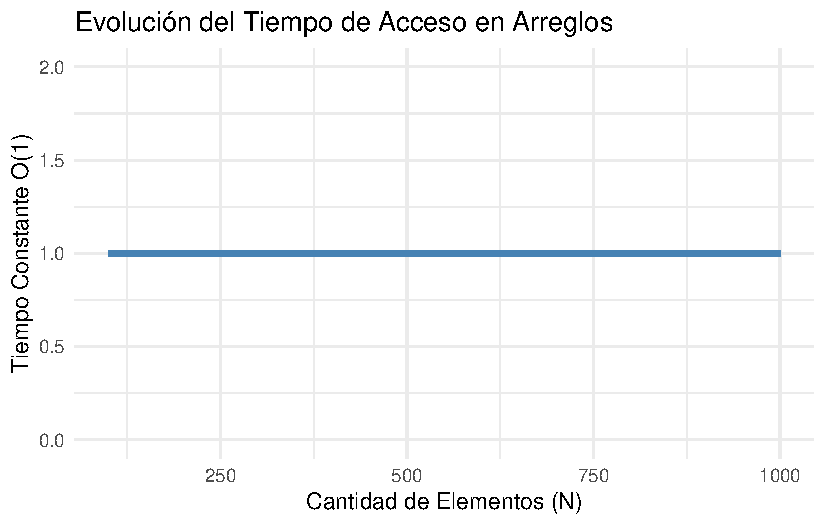
\includegraphics[keepaspectratio]{01-estructuras-estaticas_files/figure-pdf/fig-acceso-arreglo-1.pdf}}

}

\caption{\label{fig-acceso-arreglo}Tiempo de acceso constante O(1) en
arreglos estáticos al conocer la dirección exacta.}

\end{figure}%

Como observamos en la Figura~\ref{fig-acceso-arreglo}, buscar el
elemento \texttt{500} toma idéntico esfuerzo que buscar el primer
elemento. La máquina simplemente ejecuta un cálculo matemático de salto:
\texttt{Dirección\ Base\ +\ (Índice\ ×\ Tamaño\ del\ Tipo)}.

\subsection{El Lado Oscuro: Inserciones y
Eliminaciones}\label{el-lado-oscuro-inserciones-y-eliminaciones}

Si bien acceder mediante un índice es magia pura, insertar un nuevo
valor en medio del arreglo es un escenario diferente. Es similar a
intentar meter un libro ancho en medio de un estante de biblioteca que
ya está rebosante de tomos fuertemente empaquetados. Debes desplazar
manualmente uno por uno todos los libros de la derecha para abrir un
hueco.

Este corrimiento implica un tiempo que escala linealmente u
\(\mathcal{O}(N)\) en el peor de los casos, preparando el terreno para
la imperiosa necesidad de \emph{estructuras dinámicas} que analizaremos
más adelante.

\section{Archivos: Persistencia más allá de la RAM}\label{sec-archivos}

Mientras que los arreglos viven limitados al horizonte de la memoria
volátil, los \textbf{Archivos} residen en el almacenamiento secundario.
Funcionalmente, actúan como las inmensas bodegas a largo plazo de
nuestra aplicación.

Al igual que un arreglo es una tira de variables, un archivo puede
interpretarse en su abstracción más simple como un gran arreglo de bytes
apilado permanentemente.

\begin{Shaded}
\begin{Highlighting}[]
\CommentTok{\# Ejemplo ilusitrativo de cómo en Python el arreglo persistente }
\CommentTok{\# se expone como un stream lineal de datos}
\NormalTok{with }\FunctionTok{open}\NormalTok{(}\StringTok{"datos.txt"}\NormalTok{, }\StringTok{"w"}\NormalTok{) as archivo}\SpecialCharTok{:}
    \FunctionTok{archivo.write}\NormalTok{(}\StringTok{"Persistencia consolidada..."}\NormalTok{)}
\end{Highlighting}
\end{Shaded}

Interactuar físicamente con los discos magnéticos o solidos (I/O)
siempre conlleva una penalización en latencia masiva comparado con la
RAM. Por lo tanto, agrupar las peticiones (usando \emph{buffers} locales
basados en arreglos temporales rápidos) es la esencia clave para un I/O
de calidad superior.

\section{Matrices y Arreglos Multidimensionales}\label{sec-matrices}

Un paso más allá del arreglo unidimensional (vector), encontramos las
matrices. Representan datos tabulares (filas y columnas) o espacios
\(N\)-dimensionales. En memoria, la computadora sigue siendo
estrictamente lineal; no existe físicamente una ``cuadrícula 2D'' dentro
de la RAM.

Para lograr esta ilusión de multidimensionalidad, los compiladores y
lenguajes de programación utilizan técnicas de transformación
matemática, como la representación \textbf{Row-Major Order} (orden
contiguo por filas) o la instanciación de ``arreglos de arreglos'' (el
enfoque típico en Java).

\subsection{Mapeo de 2D a Memoria
Lineal}\label{mapeo-de-2d-a-memoria-lineal}

Si tenemos una matriz cuadrática de \(3 \times 3\), en un enfoque de
orden por filas, la primera fila completa ocupará las primeras 3
posiciones contiguas de memoria, seguida inmediatamente por la segunda
fila, y así sucesivamente.

La fórmula de traducción de un índice lógico \((i, j)\) a una posición
física lineal en una matriz de tamaño \(M \times N\) (filas \(\times\)
columnas), asumiendo índices basados en cero, es:

\(Posición = DirecciónBase + (i \times N + j) \times TamañoDelDato\)

Esto garantiza que el acceso a cualquier celda de la matriz siga siendo
una operación aritmética simple y, por tanto, mantenga un tiempo de
acceso \(\mathcal{O}(1)\).

\begin{Shaded}
\begin{Highlighting}[]
\CommentTok{\# Ejemplo en Python usando listas por comprensión para simular}
\CommentTok{\# una matriz (comportamiento 2D) de 3x3 inicializada en 0:}
\NormalTok{matriz }\OperatorTok{=}\NormalTok{ [[}\DecValTok{0} \ControlFlowTok{for}\NormalTok{ \_ }\KeywordTok{in} \BuiltInTok{range}\NormalTok{(}\DecValTok{3}\NormalTok{)] }\ControlFlowTok{for}\NormalTok{ \_ }\KeywordTok{in} \BuiltInTok{range}\NormalTok{(}\DecValTok{3}\NormalTok{)]}
\NormalTok{matriz[}\DecValTok{1}\NormalTok{][}\DecValTok{2}\NormalTok{] }\OperatorTok{=} \DecValTok{5} \CommentTok{\# Acceso lógico bidimensional O(1)}
\end{Highlighting}
\end{Shaded}

\section{Cadenas de Caracteres (Strings)}\label{sec-strings}

Las cadenas de texto, en su formato más fundacional (como en el lenguaje
C), no son más que arreglos estáticos de caracteres primitivos
(\texttt{char}) terminados por un carácter nulo
(\texttt{\textbackslash{}0}).

En lenguajes orientados a objetos modernos como Java y Python, la
mayoría de los \texttt{Strings} se diseñan como \textbf{objetos
inmutables}, respaldados internamente bajo el capó por un arreglo
estático de caracteres (o bytes para codificaciones como UTF-8).

\textbf{La Trampa del Rendimiento (Eficiencia \(\mathcal{O}(N^2)\))}

Esta inmutabilidad tiene una consecuencia directa en el rendimiento
algorítmico: cada vez que ``modificas'' un String (por ejemplo,
concatenando un carácter dentro de un bucle \texttt{for}), el sistema no
modifica el arreglo original porque es estático e inmutable. En su
lugar, el sistema se ve forzado a solicitar nueva memoria, crear un
\textbf{nuevo arreglo estático} más grande, y copiar secuencialmente
todos los caracteres viejos más el nuevo.

Si repites esto miles de veces, el rendimiento de tu aplicación se
desplomará drásticamente. Esta es la razón técnica por la cual, a nivel
de síntesis de software avanzado, se debe utilizar
\texttt{StringBuilder} en Java o métodos como
\texttt{\textquotesingle{}\textquotesingle{}.join(lista)} en Python
cuando se construyen concatenaciones masivas de texto.

\section{Metodologías Activas}\label{metodologuxedas-activas}

\subsection{Autoevaluación}\label{autoevaluaciuxf3n}

\begin{enumerate}
\def\labelenumi{\arabic{enumi}.}
\tightlist
\item
  \textbf{Reflexiona:} Si necesitas almacenar una lista de usuarios de
  un \emph{chat-room} activo, donde participantes se desconectan
  aleatoriamente y entran otros a diferente ritmo; ¿Qué desventajas
  concretas sufriera tu servidor intentando gestionar esas bajas si solo
  posees estructuras de tipo arreglo puro?
\item
  \textbf{Experimenta Mentalmente:} Modula la fórmula matemática de un
  arreglo \texttt{DirecciónBase\ +\ (Índice\ *\ OffsetBytes)}. ¿Qué
  ocurriría si intentaras buscar \texttt{calificaciones{[}10{]}} en el
  arreglo de 5 casillas instanciado antes? ¿Hacia donde apunta la
  memoria? (Investiga el concepto de \emph{Buffer Overflow} o excepcion
  \emph{Out of Bounds} de Java).
\end{enumerate}

\subsection{Resolución de Problemas}\label{resoluciuxf3n-de-problemas}

\textbf{El Reto de Fusión Cíclica (Merge Files)}

Imagina un caso de la vida real: tienes en posesión dos archivos
gigantes, \texttt{registros\_A.csv} y \texttt{registros\_B.csv}, y ambos
contienen columnas financieras estáticas formadas por IDs crecientes
ordenados ascendentemente (1, 2, 5\ldots{} \textbar{} 3, 4, 6\ldots).
Están ubicados en el lenta memoria secundaria, pero son colosales; no
todos los IDs caben dentro del corto cinturón RAM como arreglos masivos.

\emph{Tu misión:} Escribe pseudocódigo o diseña la arquitectura
paso-a-paso de una rutina (estilo de las que implementaríamos en Java o
Python) que logre leer ambos archivos \emph{simultáneamente} e ir
inyectando sus datos fusionados iterativamente de manera sincronizada en
un gran y final \texttt{merge.csv} ordenado, utilizando exclusivamente
de a 2 casillas temporales en tu RAM mientras iteran.

Este ejercicio fusiona lo mejor de ambos mundos: la inmensa capacidad de
iteración de flujos de archivos estáticos y punteros lógicos en arreglos
de retención. ¡Presenta tu algoritmo en el siguiente encuentro de
codiseño!

\bookmarksetup{startatroot}

\chapter{Estructuras Dinámicas}\label{estructuras-dinuxe1micas}

\bookmarksetup{startatroot}

\chapter{Introducción a las Estructuras Dinámicas en
R}\label{introducciuxf3n-a-las-estructuras-dinuxe1micas-en-r}

¡Hola! En este capítulo, nos sumergiremos en el fascinante mundo de las
estructuras de datos dinámicas. A diferencia de las estructuras
estáticas como los arrays (o vectores en R) que tienen un tamaño fijo
una vez definidos, las estructuras dinámicas pueden crecer o encogerse
durante la ejecución del programa, adaptándose a las necesidades
cambiantes de los datos.

R, con su enfoque en la manipulación de datos y su poderoso tipo
\texttt{list}, nos ofrece una gran flexibilidad. Si bien muchas de estas
estructuras dinámicas no tienen una implementación ``nativa'' y
explícita como en lenguajes de bajo nivel (como C++ o Java), entender
sus principios y cómo simularlas en R es fundamental para escribir
código eficiente y estructurado, especialmente cuando se trabaja con
datos que cambian de tamaño o cuando se necesita un control preciso
sobre el orden de procesamiento.

En este capítulo, exploraremos:

\begin{itemize}
\tightlist
\item
  \textbf{Listas Enlazadas}: Desde las simples hasta las dobles y
  circulares, comprenderemos cómo construir secuencias de elementos que
  no necesitan estar contiguos en memoria.
\item
  \textbf{Pilas (Stacks)}: Una estructura ``LIFO'' (Last-In, First-Out)
  que es esencial para tareas como la gestión de funciones o la
  evaluación de expresiones.
\item
  \textbf{Colas (Queues)}: Una estructura ``FIFO'' (First-In, First-Out)
  que simula líneas de espera y es crucial en escenarios de
  procesamiento ordenado.
\end{itemize}

Prepárate para pensar en cómo R, con su flexibilidad, puede ayudarnos a
construir estas abstracciones. Aunque a menudo podemos resolver muchos
problemas usando los tipos \texttt{vector} o \texttt{list} directamente,
comprender las estructuras dinámicas nos da una base sólida para elegir
la herramienta correcta para cada tarea y apreciar la ingeniería detrás
de las soluciones más complejas.

\begin{center}\rule{0.5\linewidth}{0.5pt}\end{center}

\bookmarksetup{startatroot}

\chapter{Listas Enlazadas}\label{listas-enlazadas}

Las listas enlazadas son una de las estructuras de datos dinámicas más
fundamentales. Consisten en una secuencia de ``nodos'', donde cada nodo
contiene un valor (o datos) y una referencia (o ``enlace'') al siguiente
nodo en la secuencia. La principal ventaja sobre los vectores es que los
elementos no necesitan estar almacenados en ubicaciones de memoria
contiguas, lo que facilita las operaciones de inserción y eliminación
sin necesidad de reasignar o desplazar grandes bloques de memoria.

En R, no tenemos ``punteros'' explícitos como en C o C++. Sin embargo,
podemos simular el comportamiento de las listas enlazadas utilizando la
flexibilidad del tipo \texttt{list} de R, donde cada ``nodo'' será una
lista que contiene el valor del dato y una referencia al siguiente nodo
(que a su vez será otra lista o \texttt{NULL}).

\section{Listas (Generales en R)}\label{listas-generales-en-r}

Antes de sumergirnos en las listas enlazadas, recordemos cómo funcionan
las listas en R, ya que son la base de nuestra simulación. Las listas de
R son colecciones ordenadas de objetos, donde los objetos pueden ser de
diferentes tipos (heterogéneos).

\begin{tcolorbox}[enhanced jigsaw, arc=.35mm, bottomrule=.15mm, bottomtitle=1mm, breakable, colback=white, colbacktitle=quarto-callout-note-color!10!white, colframe=quarto-callout-note-color-frame, coltitle=black, left=2mm, leftrule=.75mm, opacityback=0, opacitybacktitle=0.6, rightrule=.15mm, title=\textcolor{quarto-callout-note-color}{\faInfo}\hspace{0.5em}{Nota}, titlerule=0mm, toprule=.15mm, toptitle=1mm]

Las \texttt{list} de R son extremadamente flexibles y, en muchos
escenarios, pueden ser suficientes sin necesidad de implementar
explícitamente listas enlazadas. Sin embargo, para entender los
principios, las implementaremos.

\end{tcolorbox}

Crear y acceder a elementos de una lista en R es sencillo:

\begin{Shaded}
\begin{Highlighting}[]
\CommentTok{\# Crear una lista en R}
\NormalTok{mi\_lista\_r }\OtherTok{\textless{}{-}} \FunctionTok{list}\NormalTok{(}
  \AttributeTok{nombre =} \StringTok{"Alice"}\NormalTok{,}
  \AttributeTok{edad =} \DecValTok{30}\NormalTok{,}
  \AttributeTok{puntuaciones =} \FunctionTok{c}\NormalTok{(}\DecValTok{95}\NormalTok{, }\DecValTok{88}\NormalTok{, }\DecValTok{92}\NormalTok{),}
  \AttributeTok{activa =} \ConstantTok{TRUE}
\NormalTok{)}

\CommentTok{\# Acceder a elementos por nombre}
\FunctionTok{print}\NormalTok{(mi\_lista\_r}\SpecialCharTok{$}\NormalTok{nombre)}
\FunctionTok{print}\NormalTok{(mi\_lista\_r[[}\StringTok{"edad"}\NormalTok{]])}

\CommentTok{\# Acceder a elementos por posición}
\FunctionTok{print}\NormalTok{(mi\_lista\_r[[}\DecValTok{3}\NormalTok{]])}

\CommentTok{\# Modificar un elemento}
\NormalTok{mi\_lista\_r}\SpecialCharTok{$}\NormalTok{edad }\OtherTok{\textless{}{-}} \DecValTok{31}
\FunctionTok{print}\NormalTok{(mi\_lista\_r}\SpecialCharTok{$}\NormalTok{edad)}

\CommentTok{\# Añadir un nuevo elemento}
\NormalTok{mi\_lista\_r}\SpecialCharTok{$}\NormalTok{ciudad }\OtherTok{\textless{}{-}} \StringTok{"Nueva York"}
\FunctionTok{print}\NormalTok{(mi\_lista\_r)}

\CommentTok{\# Eliminar un elemento}
\NormalTok{mi\_lista\_r}\SpecialCharTok{$}\NormalTok{activa }\OtherTok{\textless{}{-}} \ConstantTok{NULL}
\FunctionTok{print}\NormalTok{(mi\_lista\_r)}
\end{Highlighting}
\end{Shaded}

\section{Listas Simples (Singly Linked
Lists)}\label{listas-simples-singly-linked-lists}

Una lista simplemente enlazada es la forma más básica de lista enlazada.
Cada nodo tiene un valor y un puntero al siguiente nodo. El último nodo
apunta a \texttt{NULL} (o \texttt{NA} en nuestra simulación en R). Solo
se puede recorrer hacia adelante.

\textbf{Estructura de un nodo:}

\begin{verbatim}
[dato | puntero_al_siguiente] -> [dato | puntero_al_siguiente] -> ... -> [dato | NULL]
\end{verbatim}

Vamos a simular esto en R:

\begin{Shaded}
\begin{Highlighting}[]
\CommentTok{\# Función para crear un nuevo nodo}
\NormalTok{crear\_nodo\_simple }\OtherTok{\textless{}{-}} \ControlFlowTok{function}\NormalTok{(valor, }\AttributeTok{siguiente =} \ConstantTok{NULL}\NormalTok{) \{}
  \FunctionTok{list}\NormalTok{(}\AttributeTok{value =}\NormalTok{ valor, }\AttributeTok{next\_node =}\NormalTok{ siguiente)}
\NormalTok{\}}

\CommentTok{\# Clase SLL (Singly Linked List) para encapsular la lógica}
\NormalTok{SinglyLinkedList }\OtherTok{\textless{}{-}}\NormalTok{ R6}\SpecialCharTok{::}\FunctionTok{R6Class}\NormalTok{(}
  \StringTok{"SinglyLinkedList"}\NormalTok{,}
  \AttributeTok{public =} \FunctionTok{list}\NormalTok{(}
    \AttributeTok{head =} \ConstantTok{NULL}\NormalTok{,}
    
    \AttributeTok{initialize =} \ControlFlowTok{function}\NormalTok{() \{}
\NormalTok{      self}\SpecialCharTok{$}\NormalTok{head }\OtherTok{\textless{}{-}} \ConstantTok{NULL}
\NormalTok{    \},}
    
    \CommentTok{\# Añadir un nodo al final de la lista}
    \AttributeTok{append =} \ControlFlowTok{function}\NormalTok{(valor) \{}
\NormalTok{      new\_node }\OtherTok{\textless{}{-}} \FunctionTok{crear\_nodo\_simple}\NormalTok{(valor)}
      \ControlFlowTok{if}\NormalTok{ (}\FunctionTok{is.null}\NormalTok{(self}\SpecialCharTok{$}\NormalTok{head)) \{}
\NormalTok{        self}\SpecialCharTok{$}\NormalTok{head }\OtherTok{\textless{}{-}}\NormalTok{ new\_node}
\NormalTok{      \} }\ControlFlowTok{else}\NormalTok{ \{}
\NormalTok{        current }\OtherTok{\textless{}{-}}\NormalTok{ self}\SpecialCharTok{$}\NormalTok{head}
        \ControlFlowTok{while}\NormalTok{ (}\SpecialCharTok{!}\FunctionTok{is.null}\NormalTok{(current}\SpecialCharTok{$}\NormalTok{next\_node)) \{}
\NormalTok{          current }\OtherTok{\textless{}{-}}\NormalTok{ current}\SpecialCharTok{$}\NormalTok{next\_node}
\NormalTok{        \}}
\NormalTok{        current}\SpecialCharTok{$}\NormalTok{next\_node }\OtherTok{\textless{}{-}}\NormalTok{ new\_node}
\NormalTok{      \}}
      \FunctionTok{invisible}\NormalTok{(self) }\CommentTok{\# Permite encadenar llamadas}
\NormalTok{    \},}
    
    \CommentTok{\# Añadir un nodo al principio de la lista}
    \AttributeTok{prepend =} \ControlFlowTok{function}\NormalTok{(valor) \{}
\NormalTok{      new\_node }\OtherTok{\textless{}{-}} \FunctionTok{crear\_nodo\_simple}\NormalTok{(valor, self}\SpecialCharTok{$}\NormalTok{head)}
\NormalTok{      self}\SpecialCharTok{$}\NormalTok{head }\OtherTok{\textless{}{-}}\NormalTok{ new\_node}
      \FunctionTok{invisible}\NormalTok{(self)}
\NormalTok{    \},}
    
    \CommentTok{\# Imprimir la lista}
    \AttributeTok{print =} \ControlFlowTok{function}\NormalTok{() \{}
\NormalTok{      nodes\_str }\OtherTok{\textless{}{-}} \FunctionTok{c}\NormalTok{()}
\NormalTok{      current }\OtherTok{\textless{}{-}}\NormalTok{ self}\SpecialCharTok{$}\NormalTok{head}
      \ControlFlowTok{while}\NormalTok{ (}\SpecialCharTok{!}\FunctionTok{is.null}\NormalTok{(current)) \{}
\NormalTok{        nodes\_str }\OtherTok{\textless{}{-}} \FunctionTok{c}\NormalTok{(nodes\_str, }\FunctionTok{as.character}\NormalTok{(current}\SpecialCharTok{$}\NormalTok{value))}
\NormalTok{        current }\OtherTok{\textless{}{-}}\NormalTok{ current}\SpecialCharTok{$}\NormalTok{next\_node}
\NormalTok{      \}}
      \FunctionTok{cat}\NormalTok{(}\StringTok{"Lista Simple: "}\NormalTok{, }\FunctionTok{paste}\NormalTok{(nodes\_str, }\AttributeTok{collapse =} \StringTok{" {-}\textgreater{} "}\NormalTok{), }\StringTok{"}\SpecialCharTok{\textbackslash{}n}\StringTok{"}\NormalTok{)}
\NormalTok{    \},}
    
    \CommentTok{\# Buscar un valor}
    \AttributeTok{find =} \ControlFlowTok{function}\NormalTok{(valor) \{}
\NormalTok{      current }\OtherTok{\textless{}{-}}\NormalTok{ self}\SpecialCharTok{$}\NormalTok{head}
      \ControlFlowTok{while}\NormalTok{ (}\SpecialCharTok{!}\FunctionTok{is.null}\NormalTok{(current)) \{}
        \ControlFlowTok{if}\NormalTok{ (}\FunctionTok{identical}\NormalTok{(current}\SpecialCharTok{$}\NormalTok{value, valor)) \{}
          \FunctionTok{return}\NormalTok{(}\ConstantTok{TRUE}\NormalTok{)}
\NormalTok{        \}}
\NormalTok{        current }\OtherTok{\textless{}{-}}\NormalTok{ current}\SpecialCharTok{$}\NormalTok{next\_node}
\NormalTok{      \}}
      \FunctionTok{return}\NormalTok{(}\ConstantTok{FALSE}\NormalTok{)}
\NormalTok{    \},}
    
    \CommentTok{\# Eliminar un nodo por valor}
    \AttributeTok{delete =} \ControlFlowTok{function}\NormalTok{(valor) \{}
      \ControlFlowTok{if}\NormalTok{ (}\FunctionTok{is.null}\NormalTok{(self}\SpecialCharTok{$}\NormalTok{head)) \{}
        \FunctionTok{return}\NormalTok{(}\FunctionTok{invisible}\NormalTok{(self))}
\NormalTok{      \}}
      
      \CommentTok{\# Si el nodo a eliminar es la cabeza}
      \ControlFlowTok{if}\NormalTok{ (}\FunctionTok{identical}\NormalTok{(self}\SpecialCharTok{$}\NormalTok{head}\SpecialCharTok{$}\NormalTok{value, valor)) \{}
\NormalTok{        self}\SpecialCharTok{$}\NormalTok{head }\OtherTok{\textless{}{-}}\NormalTok{ self}\SpecialCharTok{$}\NormalTok{head}\SpecialCharTok{$}\NormalTok{next\_node}
        \FunctionTok{return}\NormalTok{(}\FunctionTok{invisible}\NormalTok{(self))}
\NormalTok{      \}}
      
      \CommentTok{\# Buscar el nodo y su predecesor}
\NormalTok{      current }\OtherTok{\textless{}{-}}\NormalTok{ self}\SpecialCharTok{$}\NormalTok{head}
      \ControlFlowTok{while}\NormalTok{ (}\SpecialCharTok{!}\FunctionTok{is.null}\NormalTok{(current}\SpecialCharTok{$}\NormalTok{next\_node) }\SpecialCharTok{\&\&} \SpecialCharTok{!}\FunctionTok{identical}\NormalTok{(current}\SpecialCharTok{$}\NormalTok{next\_node}\SpecialCharTok{$}\NormalTok{value, valor)) \{}
\NormalTok{        current }\OtherTok{\textless{}{-}}\NormalTok{ current}\SpecialCharTok{$}\NormalTok{next\_node}
\NormalTok{      \}}
      
      \CommentTok{\# Si se encontró el nodo a eliminar}
      \ControlFlowTok{if}\NormalTok{ (}\SpecialCharTok{!}\FunctionTok{is.null}\NormalTok{(current}\SpecialCharTok{$}\NormalTok{next\_node)) \{}
\NormalTok{        current}\SpecialCharTok{$}\NormalTok{next\_node }\OtherTok{\textless{}{-}}\NormalTok{ current}\SpecialCharTok{$}\NormalTok{next\_node}\SpecialCharTok{$}\NormalTok{next\_node}
\NormalTok{      \}}
      \FunctionTok{invisible}\NormalTok{(self)}
\NormalTok{    \}}
\NormalTok{  )}
\NormalTok{)}

\CommentTok{\# Ejemplo de uso de la lista simple}
\NormalTok{sll }\OtherTok{\textless{}{-}}\NormalTok{ SinglyLinkedList}\SpecialCharTok{$}\FunctionTok{new}\NormalTok{()}

\NormalTok{sll}\SpecialCharTok{$}\FunctionTok{append}\NormalTok{(}\StringTok{"Manzana"}\NormalTok{)}\SpecialCharTok{$}\FunctionTok{append}\NormalTok{(}\StringTok{"Banana"}\NormalTok{)}\SpecialCharTok{$}\FunctionTok{append}\NormalTok{(}\StringTok{"Cereza"}\NormalTok{)}
\NormalTok{sll}\SpecialCharTok{$}\FunctionTok{print}\NormalTok{()}

\NormalTok{sll}\SpecialCharTok{$}\FunctionTok{prepend}\NormalTok{(}\StringTok{"Uva"}\NormalTok{)}
\NormalTok{sll}\SpecialCharTok{$}\FunctionTok{print}\NormalTok{()}

\FunctionTok{cat}\NormalTok{(}\StringTok{"¿Banana está en la lista?"}\NormalTok{, sll}\SpecialCharTok{$}\FunctionTok{find}\NormalTok{(}\StringTok{"Banana"}\NormalTok{), }\StringTok{"}\SpecialCharTok{\textbackslash{}n}\StringTok{"}\NormalTok{)}
\FunctionTok{cat}\NormalTok{(}\StringTok{"¿Naranja está en la lista?"}\NormalTok{, sll}\SpecialCharTok{$}\FunctionTok{find}\NormalTok{(}\StringTok{"Naranja"}\NormalTok{), }\StringTok{"}\SpecialCharTok{\textbackslash{}n}\StringTok{"}\NormalTok{)}

\NormalTok{sll}\SpecialCharTok{$}\FunctionTok{delete}\NormalTok{(}\StringTok{"Banana"}\NormalTok{)}
\NormalTok{sll}\SpecialCharTok{$}\FunctionTok{print}\NormalTok{()}

\NormalTok{sll}\SpecialCharTok{$}\FunctionTok{delete}\NormalTok{(}\StringTok{"Uva"}\NormalTok{) }\CommentTok{\# Eliminar la cabeza}
\NormalTok{sll}\SpecialCharTok{$}\FunctionTok{print}\NormalTok{()}

\NormalTok{sll}\SpecialCharTok{$}\FunctionTok{delete}\NormalTok{(}\StringTok{"Cereza"}\NormalTok{) }\CommentTok{\# Eliminar el último}
\NormalTok{sll}\SpecialCharTok{$}\FunctionTok{print}\NormalTok{()}

\NormalTok{sll}\SpecialCharTok{$}\FunctionTok{delete}\NormalTok{(}\StringTok{"Manzana"}\NormalTok{) }\CommentTok{\# Eliminar el último que queda}
\NormalTok{sll}\SpecialCharTok{$}\FunctionTok{print}\NormalTok{()}
\end{Highlighting}
\end{Shaded}

\begin{tcolorbox}[enhanced jigsaw, arc=.35mm, bottomrule=.15mm, bottomtitle=1mm, breakable, colback=white, colbacktitle=quarto-callout-note-color!10!white, colframe=quarto-callout-note-color-frame, coltitle=black, left=2mm, leftrule=.75mm, opacityback=0, opacitybacktitle=0.6, rightrule=.15mm, title=\textcolor{quarto-callout-note-color}{\faInfo}\hspace{0.5em}{Nota}, titlerule=0mm, toprule=.15mm, toptitle=1mm]

\textbf{Nota sobre la simulación en R:} Al crear un nodo como
\texttt{list(value\ =\ valor,\ next\_node\ =\ siguiente)}, el
\texttt{siguiente} es una referencia \emph{copia} del objeto
\texttt{list} completo. R gestiona la memoria y las referencias de
objetos de manera diferente a lenguajes como C, donde un puntero es una
dirección de memoria. Sin embargo, para entender el comportamiento
lógico de las listas enlazadas, esta simulación es muy efectiva. Para
grandes volúmenes de datos y operaciones frecuentes, las \texttt{list}
nativas de R o estructuras más optimizadas podrían ser preferibles por
rendimiento.

\end{tcolorbox}

\section{Listas Dobles (Doubly Linked
Lists)}\label{listas-dobles-doubly-linked-lists}

Una lista doblemente enlazada mejora la lista simple añadiendo un
puntero al nodo \emph{anterior} además del puntero al siguiente nodo.
Esto permite recorrer la lista en ambas direcciones y simplifica ciertas
operaciones, como la eliminación de un nodo (ya que no necesitamos
mantener un puntero al predecesor).

\textbf{Estructura de un nodo:}

\begin{verbatim}
NULL <- [puntero_anterior | dato | puntero_siguiente] <-> ... <-> [puntero_anterior | dato | puntero_siguiente] -> NULL
\end{verbatim}

\begin{Shaded}
\begin{Highlighting}[]
\CommentTok{\# Función para crear un nuevo nodo doble}
\NormalTok{crear\_nodo\_doble }\OtherTok{\textless{}{-}} \ControlFlowTok{function}\NormalTok{(valor, }\AttributeTok{anterior =} \ConstantTok{NULL}\NormalTok{, }\AttributeTok{siguiente =} \ConstantTok{NULL}\NormalTok{) \{}
  \FunctionTok{list}\NormalTok{(}\AttributeTok{value =}\NormalTok{ valor, }\AttributeTok{prev\_node =}\NormalTok{ anterior, }\AttributeTok{next\_node =}\NormalTok{ siguiente)}
\NormalTok{\}}

\CommentTok{\# Clase DLL (Doubly Linked List)}
\NormalTok{DoublyLinkedList }\OtherTok{\textless{}{-}}\NormalTok{ R6}\SpecialCharTok{::}\FunctionTok{R6Class}\NormalTok{(}
  \StringTok{"DoublyLinkedList"}\NormalTok{,}
  \AttributeTok{public =} \FunctionTok{list}\NormalTok{(}
    \AttributeTok{head =} \ConstantTok{NULL}\NormalTok{,}
    \AttributeTok{tail =} \ConstantTok{NULL}\NormalTok{, }\CommentTok{\# Mantenemos un puntero a la cola para inserciones rápidas al final}
    
    \AttributeTok{initialize =} \ControlFlowTok{function}\NormalTok{() \{}
\NormalTok{      self}\SpecialCharTok{$}\NormalTok{head }\OtherTok{\textless{}{-}} \ConstantTok{NULL}
\NormalTok{      self}\SpecialCharTok{$}\NormalTok{tail }\OtherTok{\textless{}{-}} \ConstantTok{NULL}
\NormalTok{    \},}
    
    \CommentTok{\# Añadir un nodo al final}
    \AttributeTok{append =} \ControlFlowTok{function}\NormalTok{(valor) \{}
\NormalTok{      new\_node }\OtherTok{\textless{}{-}} \FunctionTok{crear\_nodo\_doble}\NormalTok{(valor)}
      \ControlFlowTok{if}\NormalTok{ (}\FunctionTok{is.null}\NormalTok{(self}\SpecialCharTok{$}\NormalTok{head)) \{}
\NormalTok{        self}\SpecialCharTok{$}\NormalTok{head }\OtherTok{\textless{}{-}}\NormalTok{ new\_node}
\NormalTok{        self}\SpecialCharTok{$}\NormalTok{tail }\OtherTok{\textless{}{-}}\NormalTok{ new\_node}
\NormalTok{      \} }\ControlFlowTok{else}\NormalTok{ \{}
\NormalTok{        self}\SpecialCharTok{$}\NormalTok{tail}\SpecialCharTok{$}\NormalTok{next\_node }\OtherTok{\textless{}{-}}\NormalTok{ new\_node}
\NormalTok{        new\_node}\SpecialCharTok{$}\NormalTok{prev\_node }\OtherTok{\textless{}{-}}\NormalTok{ self}\SpecialCharTok{$}\NormalTok{tail}
\NormalTok{        self}\SpecialCharTok{$}\NormalTok{tail }\OtherTok{\textless{}{-}}\NormalTok{ new\_node}
\NormalTok{      \}}
      \FunctionTok{invisible}\NormalTok{(self)}
\NormalTok{    \},}
    
    \CommentTok{\# Añadir un nodo al principio}
    \AttributeTok{prepend =} \ControlFlowTok{function}\NormalTok{(valor) \{}
\NormalTok{      new\_node }\OtherTok{\textless{}{-}} \FunctionTok{crear\_nodo\_doble}\NormalTok{(valor, }\AttributeTok{siguiente =}\NormalTok{ self}\SpecialCharTok{$}\NormalTok{head)}
      \ControlFlowTok{if}\NormalTok{ (}\FunctionTok{is.null}\NormalTok{(self}\SpecialCharTok{$}\NormalTok{head)) \{}
\NormalTok{        self}\SpecialCharTok{$}\NormalTok{head }\OtherTok{\textless{}{-}}\NormalTok{ new\_node}
\NormalTok{        self}\SpecialCharTok{$}\NormalTok{tail }\OtherTok{\textless{}{-}}\NormalTok{ new\_node}
\NormalTok{      \} }\ControlFlowTok{else}\NormalTok{ \{}
\NormalTok{        self}\SpecialCharTok{$}\NormalTok{head}\SpecialCharTok{$}\NormalTok{prev\_node }\OtherTok{\textless{}{-}}\NormalTok{ new\_node}
\NormalTok{        self}\SpecialCharTok{$}\NormalTok{head }\OtherTok{\textless{}{-}}\NormalTok{ new\_node}
\NormalTok{      \}}
      \FunctionTok{invisible}\NormalTok{(self)}
\NormalTok{    \},}
    
    \CommentTok{\# Imprimir la lista (hacia adelante)}
    \AttributeTok{print\_forward =} \ControlFlowTok{function}\NormalTok{() \{}
\NormalTok{      nodes\_str }\OtherTok{\textless{}{-}} \FunctionTok{c}\NormalTok{()}
\NormalTok{      current }\OtherTok{\textless{}{-}}\NormalTok{ self}\SpecialCharTok{$}\NormalTok{head}
      \ControlFlowTok{while}\NormalTok{ (}\SpecialCharTok{!}\FunctionTok{is.null}\NormalTok{(current)) \{}
\NormalTok{        nodes\_str }\OtherTok{\textless{}{-}} \FunctionTok{c}\NormalTok{(nodes\_str, }\FunctionTok{as.character}\NormalTok{(current}\SpecialCharTok{$}\NormalTok{value))}
\NormalTok{        current }\OtherTok{\textless{}{-}}\NormalTok{ current}\SpecialCharTok{$}\NormalTok{next\_node}
\NormalTok{      \}}
      \FunctionTok{cat}\NormalTok{(}\StringTok{"Lista Doble (Adelante): "}\NormalTok{, }\FunctionTok{paste}\NormalTok{(nodes\_str, }\AttributeTok{collapse =} \StringTok{" \textless{}{-}\textgreater{} "}\NormalTok{), }\StringTok{"}\SpecialCharTok{\textbackslash{}n}\StringTok{"}\NormalTok{)}
\NormalTok{    \},}
    
    \CommentTok{\# Imprimir la lista (hacia atrás)}
    \AttributeTok{print\_backward =} \ControlFlowTok{function}\NormalTok{() \{}
\NormalTok{      nodes\_str }\OtherTok{\textless{}{-}} \FunctionTok{c}\NormalTok{()}
\NormalTok{      current }\OtherTok{\textless{}{-}}\NormalTok{ self}\SpecialCharTok{$}\NormalTok{tail}
      \ControlFlowTok{while}\NormalTok{ (}\SpecialCharTok{!}\FunctionTok{is.null}\NormalTok{(current)) \{}
\NormalTok{        nodes\_str }\OtherTok{\textless{}{-}} \FunctionTok{c}\NormalTok{(nodes\_str, }\FunctionTok{as.character}\NormalTok{(current}\SpecialCharTok{$}\NormalTok{value))}
\NormalTok{        current }\OtherTok{\textless{}{-}}\NormalTok{ current}\SpecialCharTok{$}\NormalTok{prev\_node}
\NormalTok{      \}}
      \FunctionTok{cat}\NormalTok{(}\StringTok{"Lista Doble (Atrás): "}\NormalTok{, }\FunctionTok{paste}\NormalTok{(nodes\_str, }\AttributeTok{collapse =} \StringTok{" \textless{}{-}\textgreater{} "}\NormalTok{), }\StringTok{"}\SpecialCharTok{\textbackslash{}n}\StringTok{"}\NormalTok{)}
\NormalTok{    \},}
    
    \CommentTok{\# Eliminar un nodo por valor}
    \AttributeTok{delete =} \ControlFlowTok{function}\NormalTok{(valor) \{}
      \ControlFlowTok{if}\NormalTok{ (}\FunctionTok{is.null}\NormalTok{(self}\SpecialCharTok{$}\NormalTok{head)) \{}
        \FunctionTok{return}\NormalTok{(}\FunctionTok{invisible}\NormalTok{(self))}
\NormalTok{      \}}
      
\NormalTok{      current }\OtherTok{\textless{}{-}}\NormalTok{ self}\SpecialCharTok{$}\NormalTok{head}
      \ControlFlowTok{while}\NormalTok{ (}\SpecialCharTok{!}\FunctionTok{is.null}\NormalTok{(current) }\SpecialCharTok{\&\&} \SpecialCharTok{!}\FunctionTok{identical}\NormalTok{(current}\SpecialCharTok{$}\NormalTok{value, valor)) \{}
\NormalTok{        current }\OtherTok{\textless{}{-}}\NormalTok{ current}\SpecialCharTok{$}\NormalTok{next\_node}
\NormalTok{      \}}
      
      \CommentTok{\# Si el valor no se encontró}
      \ControlFlowTok{if}\NormalTok{ (}\FunctionTok{is.null}\NormalTok{(current)) \{}
        \FunctionTok{return}\NormalTok{(}\FunctionTok{invisible}\NormalTok{(self))}
\NormalTok{      \}}
      
      \CommentTok{\# Si el nodo a eliminar es la cabeza}
      \ControlFlowTok{if}\NormalTok{ (}\FunctionTok{is.null}\NormalTok{(current}\SpecialCharTok{$}\NormalTok{prev\_node)) \{}
\NormalTok{        self}\SpecialCharTok{$}\NormalTok{head }\OtherTok{\textless{}{-}}\NormalTok{ current}\SpecialCharTok{$}\NormalTok{next\_node}
        \ControlFlowTok{if}\NormalTok{ (}\SpecialCharTok{!}\FunctionTok{is.null}\NormalTok{(self}\SpecialCharTok{$}\NormalTok{head)) \{}
\NormalTok{          self}\SpecialCharTok{$}\NormalTok{head}\SpecialCharTok{$}\NormalTok{prev\_node }\OtherTok{\textless{}{-}} \ConstantTok{NULL}
\NormalTok{        \} }\ControlFlowTok{else}\NormalTok{ \{ }\CommentTok{\# Si la lista queda vacía}
\NormalTok{          self}\SpecialCharTok{$}\NormalTok{tail }\OtherTok{\textless{}{-}} \ConstantTok{NULL}
\NormalTok{        \}}
\NormalTok{      \} }
      \CommentTok{\# Si el nodo a eliminar es la cola}
      \ControlFlowTok{else} \ControlFlowTok{if}\NormalTok{ (}\FunctionTok{is.null}\NormalTok{(current}\SpecialCharTok{$}\NormalTok{next\_node)) \{}
\NormalTok{        self}\SpecialCharTok{$}\NormalTok{tail }\OtherTok{\textless{}{-}}\NormalTok{ current}\SpecialCharTok{$}\NormalTok{prev\_node}
        \ControlFlowTok{if}\NormalTok{ (}\SpecialCharTok{!}\FunctionTok{is.null}\NormalTok{(self}\SpecialCharTok{$}\NormalTok{tail)) \{}
\NormalTok{          self}\SpecialCharTok{$}\NormalTok{tail}\SpecialCharTok{$}\NormalTok{next\_node }\OtherTok{\textless{}{-}} \ConstantTok{NULL}
\NormalTok{        \} }\ControlFlowTok{else}\NormalTok{ \{ }\CommentTok{\# Si la lista queda vacía}
\NormalTok{          self}\SpecialCharTok{$}\NormalTok{head }\OtherTok{\textless{}{-}} \ConstantTok{NULL}
\NormalTok{        \}}
\NormalTok{      \}}
      \CommentTok{\# Si el nodo está en el medio}
      \ControlFlowTok{else}\NormalTok{ \{}
\NormalTok{        current}\SpecialCharTok{$}\NormalTok{prev\_node}\SpecialCharTok{$}\NormalTok{next\_node }\OtherTok{\textless{}{-}}\NormalTok{ current}\SpecialCharTok{$}\NormalTok{next\_node}
\NormalTok{        current}\SpecialCharTok{$}\NormalTok{next\_node}\SpecialCharTok{$}\NormalTok{prev\_node }\OtherTok{\textless{}{-}}\NormalTok{ current}\SpecialCharTok{$}\NormalTok{prev\_node}
\NormalTok{      \}}
      \FunctionTok{invisible}\NormalTok{(self)}
\NormalTok{    \}}
\NormalTok{  )}
\NormalTok{)}

\CommentTok{\# Ejemplo de uso de la lista doble}
\NormalTok{dll }\OtherTok{\textless{}{-}}\NormalTok{ DoublyLinkedList}\SpecialCharTok{$}\FunctionTok{new}\NormalTok{()}

\NormalTok{dll}\SpecialCharTok{$}\FunctionTok{append}\NormalTok{(}\StringTok{"Uno"}\NormalTok{)}\SpecialCharTok{$}\FunctionTok{append}\NormalTok{(}\StringTok{"Dos"}\NormalTok{)}\SpecialCharTok{$}\FunctionTok{append}\NormalTok{(}\StringTok{"Tres"}\NormalTok{)}
\NormalTok{dll}\SpecialCharTok{$}\FunctionTok{print\_forward}\NormalTok{()}
\NormalTok{dll}\SpecialCharTok{$}\FunctionTok{print\_backward}\NormalTok{()}

\NormalTok{dll}\SpecialCharTok{$}\FunctionTok{prepend}\NormalTok{(}\StringTok{"Cero"}\NormalTok{)}
\NormalTok{dll}\SpecialCharTok{$}\FunctionTok{print\_forward}\NormalTok{()}

\NormalTok{dll}\SpecialCharTok{$}\FunctionTok{delete}\NormalTok{(}\StringTok{"Dos"}\NormalTok{)}
\NormalTok{dll}\SpecialCharTok{$}\FunctionTok{print\_forward}\NormalTok{()}
\NormalTok{dll}\SpecialCharTok{$}\FunctionTok{print\_backward}\NormalTok{()}

\NormalTok{dll}\SpecialCharTok{$}\FunctionTok{delete}\NormalTok{(}\StringTok{"Cero"}\NormalTok{) }\CommentTok{\# Eliminar la cabeza}
\NormalTok{dll}\SpecialCharTok{$}\FunctionTok{print\_forward}\NormalTok{()}

\NormalTok{dll}\SpecialCharTok{$}\FunctionTok{delete}\NormalTok{(}\StringTok{"Tres"}\NormalTok{) }\CommentTok{\# Eliminar la cola}
\NormalTok{dll}\SpecialCharTok{$}\FunctionTok{print\_forward}\NormalTok{()}

\NormalTok{dll}\SpecialCharTok{$}\FunctionTok{delete}\NormalTok{(}\StringTok{"Uno"}\NormalTok{) }\CommentTok{\# Eliminar el último}
\NormalTok{dll}\SpecialCharTok{$}\FunctionTok{print\_forward}\NormalTok{()}
\NormalTok{dll}\SpecialCharTok{$}\FunctionTok{print\_backward}\NormalTok{() }\CommentTok{\# La lista está vacía}
\end{Highlighting}
\end{Shaded}

\section{Listas Circulares (Circular Linked
Lists)}\label{listas-circulares-circular-linked-lists}

Una lista circular es una lista enlazada donde el último nodo apunta al
primer nodo, creando un ciclo. Puede ser simplemente o doblemente
enlazada, pero la característica clave es el cierre del ciclo. Esto es
útil para estructuras que no tienen un ``principio'' o ``fin'' natural,
o donde se necesita un acceso continuo a los elementos (por ejemplo, en
la planificación de procesos de un sistema operativo).

\textbf{Estructura (Simple Circular):}

\begin{verbatim}
[dato | puntero_siguiente] -> [dato | puntero_siguiente] -> ... -> [dato | puntero_al_primero]
   ^                                                                     |
   |_____________________________________________________________________|
\end{verbatim}

\begin{Shaded}
\begin{Highlighting}[]
\CommentTok{\# Clase CLL (Circular Linked List)}
\NormalTok{CircularLinkedList }\OtherTok{\textless{}{-}}\NormalTok{ R6}\SpecialCharTok{::}\FunctionTok{R6Class}\NormalTok{(}
  \StringTok{"CircularLinkedList"}\NormalTok{,}
  \AttributeTok{public =} \FunctionTok{list}\NormalTok{(}
    \AttributeTok{head =} \ConstantTok{NULL}\NormalTok{,}
    
    \AttributeTok{initialize =} \ControlFlowTok{function}\NormalTok{() \{}
\NormalTok{      self}\SpecialCharTok{$}\NormalTok{head }\OtherTok{\textless{}{-}} \ConstantTok{NULL}
\NormalTok{    \},}
    
    \CommentTok{\# Añadir un nodo al final (mantiene el orden circular)}
    \AttributeTok{append =} \ControlFlowTok{function}\NormalTok{(valor) \{}
\NormalTok{      new\_node }\OtherTok{\textless{}{-}} \FunctionTok{crear\_nodo\_simple}\NormalTok{(valor) }\CommentTok{\# Usamos el nodo simple para la base}
      \ControlFlowTok{if}\NormalTok{ (}\FunctionTok{is.null}\NormalTok{(self}\SpecialCharTok{$}\NormalTok{head)) \{}
\NormalTok{        self}\SpecialCharTok{$}\NormalTok{head }\OtherTok{\textless{}{-}}\NormalTok{ new\_node}
\NormalTok{        new\_node}\SpecialCharTok{$}\NormalTok{next\_node }\OtherTok{\textless{}{-}}\NormalTok{ self}\SpecialCharTok{$}\NormalTok{head }\CommentTok{\# Apunta a sí mismo para formar el círculo}
\NormalTok{      \} }\ControlFlowTok{else}\NormalTok{ \{}
\NormalTok{        current }\OtherTok{\textless{}{-}}\NormalTok{ self}\SpecialCharTok{$}\NormalTok{head}
        \CommentTok{\# Recorrer hasta el nodo justo antes de la cabeza (el actual "final")}
        \ControlFlowTok{while}\NormalTok{ (}\SpecialCharTok{!}\FunctionTok{identical}\NormalTok{(current}\SpecialCharTok{$}\NormalTok{next\_node, self}\SpecialCharTok{$}\NormalTok{head)) \{}
\NormalTok{          current }\OtherTok{\textless{}{-}}\NormalTok{ current}\SpecialCharTok{$}\NormalTok{next\_node}
\NormalTok{        \}}
\NormalTok{        current}\SpecialCharTok{$}\NormalTok{next\_node }\OtherTok{\textless{}{-}}\NormalTok{ new\_node}
\NormalTok{        new\_node}\SpecialCharTok{$}\NormalTok{next\_node }\OtherTok{\textless{}{-}}\NormalTok{ self}\SpecialCharTok{$}\NormalTok{head }\CommentTok{\# El nuevo nodo apunta a la cabeza}
\NormalTok{      \}}
      \FunctionTok{invisible}\NormalTok{(self)}
\NormalTok{    \},}
    
    \CommentTok{\# Imprimir la lista (recorre una vez el círculo)}
    \AttributeTok{print =} \ControlFlowTok{function}\NormalTok{() \{}
      \ControlFlowTok{if}\NormalTok{ (}\FunctionTok{is.null}\NormalTok{(self}\SpecialCharTok{$}\NormalTok{head)) \{}
        \FunctionTok{cat}\NormalTok{(}\StringTok{"Lista Circular: Vacía}\SpecialCharTok{\textbackslash{}n}\StringTok{"}\NormalTok{)}
        \FunctionTok{return}\NormalTok{(}\FunctionTok{invisible}\NormalTok{(self))}
\NormalTok{      \}}
      
\NormalTok{      nodes\_str }\OtherTok{\textless{}{-}} \FunctionTok{c}\NormalTok{()}
\NormalTok{      current }\OtherTok{\textless{}{-}}\NormalTok{ self}\SpecialCharTok{$}\NormalTok{head}
      \ControlFlowTok{repeat}\NormalTok{ \{}
\NormalTok{        nodes\_str }\OtherTok{\textless{}{-}} \FunctionTok{c}\NormalTok{(nodes\_str, }\FunctionTok{as.character}\NormalTok{(current}\SpecialCharTok{$}\NormalTok{value))}
\NormalTok{        current }\OtherTok{\textless{}{-}}\NormalTok{ current}\SpecialCharTok{$}\NormalTok{next\_node}
        \ControlFlowTok{if}\NormalTok{ (}\FunctionTok{identical}\NormalTok{(current, self}\SpecialCharTok{$}\NormalTok{head)) \{ }\CommentTok{\# Detener cuando volvemos a la cabeza}
          \ControlFlowTok{break}
\NormalTok{        \}}
\NormalTok{      \}}
      \FunctionTok{cat}\NormalTok{(}\StringTok{"Lista Circular: "}\NormalTok{, }\FunctionTok{paste}\NormalTok{(nodes\_str, }\AttributeTok{collapse =} \StringTok{" {-}\textgreater{} "}\NormalTok{), }\StringTok{" {-}\textgreater{} (vuelve a "}\NormalTok{, nodes\_str[}\DecValTok{1}\NormalTok{], }\StringTok{")}\SpecialCharTok{\textbackslash{}n}\StringTok{"}\NormalTok{)}
\NormalTok{    \},}
    
    \CommentTok{\# Eliminar un nodo por valor}
    \AttributeTok{delete =} \ControlFlowTok{function}\NormalTok{(valor) \{}
      \ControlFlowTok{if}\NormalTok{ (}\FunctionTok{is.null}\NormalTok{(self}\SpecialCharTok{$}\NormalTok{head)) \{}
        \FunctionTok{return}\NormalTok{(}\FunctionTok{invisible}\NormalTok{(self))}
\NormalTok{      \}}
      
      \CommentTok{\# Si la lista tiene un solo nodo}
      \ControlFlowTok{if}\NormalTok{ (}\FunctionTok{identical}\NormalTok{(self}\SpecialCharTok{$}\NormalTok{head}\SpecialCharTok{$}\NormalTok{next\_node, self}\SpecialCharTok{$}\NormalTok{head) }\SpecialCharTok{\&\&} \FunctionTok{identical}\NormalTok{(self}\SpecialCharTok{$}\NormalTok{head}\SpecialCharTok{$}\NormalTok{value, valor)) \{}
\NormalTok{        self}\SpecialCharTok{$}\NormalTok{head }\OtherTok{\textless{}{-}} \ConstantTok{NULL}
        \FunctionTok{return}\NormalTok{(}\FunctionTok{invisible}\NormalTok{(self))}
\NormalTok{      \}}
      
\NormalTok{      current }\OtherTok{\textless{}{-}}\NormalTok{ self}\SpecialCharTok{$}\NormalTok{head}
\NormalTok{      prev }\OtherTok{\textless{}{-}} \ConstantTok{NULL}
      
      \CommentTok{\# Buscar el nodo a eliminar}
      \ControlFlowTok{repeat}\NormalTok{ \{}
        \ControlFlowTok{if}\NormalTok{ (}\FunctionTok{identical}\NormalTok{(current}\SpecialCharTok{$}\NormalTok{value, valor)) \{}
          \ControlFlowTok{break} \CommentTok{\# Se encontró el nodo}
\NormalTok{        \}}
\NormalTok{        prev }\OtherTok{\textless{}{-}}\NormalTok{ current}
\NormalTok{        current }\OtherTok{\textless{}{-}}\NormalTok{ current}\SpecialCharTok{$}\NormalTok{next\_node}
        \ControlFlowTok{if}\NormalTok{ (}\FunctionTok{identical}\NormalTok{(current, self}\SpecialCharTok{$}\NormalTok{head)) \{ }\CommentTok{\# Se recorrió toda la lista y no se encontró}
          \FunctionTok{return}\NormalTok{(}\FunctionTok{invisible}\NormalTok{(self))}
\NormalTok{        \}}
\NormalTok{      \}}
      
      \CommentTok{\# Si el nodo a eliminar es la cabeza}
      \ControlFlowTok{if}\NormalTok{ (}\FunctionTok{identical}\NormalTok{(current, self}\SpecialCharTok{$}\NormalTok{head)) \{}
        \CommentTok{\# Encontrar el último nodo para actualizar su puntero}
\NormalTok{        temp\_tail }\OtherTok{\textless{}{-}}\NormalTok{ self}\SpecialCharTok{$}\NormalTok{head}
        \ControlFlowTok{while}\NormalTok{ (}\SpecialCharTok{!}\FunctionTok{identical}\NormalTok{(temp\_tail}\SpecialCharTok{$}\NormalTok{next\_node, self}\SpecialCharTok{$}\NormalTok{head)) \{}
\NormalTok{          temp\_tail }\OtherTok{\textless{}{-}}\NormalTok{ temp\_tail}\SpecialCharTok{$}\NormalTok{next\_node}
\NormalTok{        \}}
\NormalTok{        self}\SpecialCharTok{$}\NormalTok{head }\OtherTok{\textless{}{-}}\NormalTok{ self}\SpecialCharTok{$}\NormalTok{head}\SpecialCharTok{$}\NormalTok{next\_node}
\NormalTok{        temp\_tail}\SpecialCharTok{$}\NormalTok{next\_node }\OtherTok{\textless{}{-}}\NormalTok{ self}\SpecialCharTok{$}\NormalTok{head}
\NormalTok{      \} }\ControlFlowTok{else}\NormalTok{ \{ }\CommentTok{\# El nodo a eliminar no es la cabeza}
\NormalTok{        prev}\SpecialCharTok{$}\NormalTok{next\_node }\OtherTok{\textless{}{-}}\NormalTok{ current}\SpecialCharTok{$}\NormalTok{next\_node}
\NormalTok{      \}}
      \FunctionTok{invisible}\NormalTok{(self)}
\NormalTok{    \}}
\NormalTok{  )}
\NormalTok{)}

\CommentTok{\# Ejemplo de uso de la lista circular}
\NormalTok{cll }\OtherTok{\textless{}{-}}\NormalTok{ CircularLinkedList}\SpecialCharTok{$}\FunctionTok{new}\NormalTok{()}

\NormalTok{cll}\SpecialCharTok{$}\FunctionTok{append}\NormalTok{(}\StringTok{"Alfa"}\NormalTok{)}\SpecialCharTok{$}\FunctionTok{append}\NormalTok{(}\StringTok{"Beta"}\NormalTok{)}\SpecialCharTok{$}\FunctionTok{append}\NormalTok{(}\StringTok{"Gamma"}\NormalTok{)}
\NormalTok{cll}\SpecialCharTok{$}\FunctionTok{print}\NormalTok{()}

\NormalTok{cll}\SpecialCharTok{$}\FunctionTok{delete}\NormalTok{(}\StringTok{"Beta"}\NormalTok{)}
\NormalTok{cll}\SpecialCharTok{$}\FunctionTok{print}\NormalTok{()}

\NormalTok{cll}\SpecialCharTok{$}\FunctionTok{delete}\NormalTok{(}\StringTok{"Alfa"}\NormalTok{) }\CommentTok{\# Eliminar la cabeza}
\NormalTok{cll}\SpecialCharTok{$}\FunctionTok{print}\NormalTok{()}

\NormalTok{cll}\SpecialCharTok{$}\FunctionTok{delete}\NormalTok{(}\StringTok{"Gamma"}\NormalTok{) }\CommentTok{\# Eliminar el último que queda}
\NormalTok{cll}\SpecialCharTok{$}\FunctionTok{print}\NormalTok{()}

\NormalTok{cll}\SpecialCharTok{$}\FunctionTok{append}\NormalTok{(}\StringTok{"Único"}\NormalTok{)}
\NormalTok{cll}\SpecialCharTok{$}\FunctionTok{print}\NormalTok{()}
\NormalTok{cll}\SpecialCharTok{$}\FunctionTok{delete}\NormalTok{(}\StringTok{"Único"}\NormalTok{)}
\NormalTok{cll}\SpecialCharTok{$}\FunctionTok{print}\NormalTok{() }\CommentTok{\# La lista está vacía}
\end{Highlighting}
\end{Shaded}

\begin{center}\rule{0.5\linewidth}{0.5pt}\end{center}

\bookmarksetup{startatroot}

\chapter{Pilas (Stacks)}\label{pilas-stacks}

Una Pila es una estructura de datos lineal que sigue el principio
``LIFO'' (Last-In, First-Out), es decir, el último elemento añadido es
el primero en ser eliminado. Piensa en una pila de platos: solo puedes
añadir un plato encima y solo puedes quitar el plato de más arriba.

Las operaciones principales de una pila son:

\begin{itemize}
\tightlist
\item
  \textbf{Push}: Añadir un elemento a la parte superior de la pila.
\item
  \textbf{Pop}: Eliminar y devolver el elemento de la parte superior de
  la pila.
\item
  \textbf{Peek/Top}: Devolver el elemento de la parte superior sin
  eliminarlo.
\item
  \textbf{isEmpty}: Comprobar si la pila está vacía.
\item
  \textbf{Size}: Devolver el número de elementos en la pila.
\end{itemize}

En R, podemos implementar una pila de manera muy eficiente usando un
\texttt{vector} o una \texttt{list} estándar, aprovechando que las
operaciones de añadir/eliminar al final de un vector/lista son muy
rápidas.

\begin{Shaded}
\begin{Highlighting}[]
\CommentTok{\# Clase Stack}
\NormalTok{Stack }\OtherTok{\textless{}{-}}\NormalTok{ R6}\SpecialCharTok{::}\FunctionTok{R6Class}\NormalTok{(}
  \StringTok{"Stack"}\NormalTok{,}
  \AttributeTok{public =} \FunctionTok{list}\NormalTok{(}
    \AttributeTok{elements =} \ConstantTok{NULL}\NormalTok{,}
    
    \AttributeTok{initialize =} \ControlFlowTok{function}\NormalTok{() \{}
\NormalTok{      self}\SpecialCharTok{$}\NormalTok{elements }\OtherTok{\textless{}{-}} \FunctionTok{list}\NormalTok{() }\CommentTok{\# Usamos una lista para mayor flexibilidad de tipos}
\NormalTok{    \},}
    
    \CommentTok{\# Añadir un elemento a la pila (Push)}
    \AttributeTok{push =} \ControlFlowTok{function}\NormalTok{(item) \{}
\NormalTok{      self}\SpecialCharTok{$}\NormalTok{elements }\OtherTok{\textless{}{-}} \FunctionTok{c}\NormalTok{(self}\SpecialCharTok{$}\NormalTok{elements, }\FunctionTok{list}\NormalTok{(item)) }\CommentTok{\# Añadir al final}
      \FunctionTok{invisible}\NormalTok{(self)}
\NormalTok{    \},}
    
    \CommentTok{\# Eliminar y devolver el elemento superior (Pop)}
    \AttributeTok{pop =} \ControlFlowTok{function}\NormalTok{() \{}
      \ControlFlowTok{if}\NormalTok{ (self}\SpecialCharTok{$}\FunctionTok{is\_empty}\NormalTok{()) \{}
        \FunctionTok{stop}\NormalTok{(}\StringTok{"La pila está vacía, no se puede hacer pop."}\NormalTok{)}
\NormalTok{      \}}
\NormalTok{      last\_index }\OtherTok{\textless{}{-}} \FunctionTok{length}\NormalTok{(self}\SpecialCharTok{$}\NormalTok{elements)}
\NormalTok{      item }\OtherTok{\textless{}{-}}\NormalTok{ self}\SpecialCharTok{$}\NormalTok{elements[[last\_index]]}
\NormalTok{      self}\SpecialCharTok{$}\NormalTok{elements }\OtherTok{\textless{}{-}}\NormalTok{ self}\SpecialCharTok{$}\NormalTok{elements[}\SpecialCharTok{{-}}\NormalTok{last\_index] }\CommentTok{\# Eliminar el último}
      \FunctionTok{return}\NormalTok{(item)}
\NormalTok{    \},}
    
    \CommentTok{\# Devolver el elemento superior sin eliminarlo (Peek/Top)}
    \AttributeTok{peek =} \ControlFlowTok{function}\NormalTok{() \{}
      \ControlFlowTok{if}\NormalTok{ (self}\SpecialCharTok{$}\FunctionTok{is\_empty}\NormalTok{()) \{}
        \FunctionTok{return}\NormalTok{(}\ConstantTok{NULL}\NormalTok{) }\CommentTok{\# O podrías lanzar un error, dependiendo del diseño}
\NormalTok{      \}}
      \FunctionTok{return}\NormalTok{(self}\SpecialCharTok{$}\NormalTok{elements[[}\FunctionTok{length}\NormalTok{(self}\SpecialCharTok{$}\NormalTok{elements)]])}
\NormalTok{    \},}
    
    \CommentTok{\# Comprobar si la pila está vacía}
    \AttributeTok{is\_empty =} \ControlFlowTok{function}\NormalTok{() \{}
      \FunctionTok{return}\NormalTok{(}\FunctionTok{length}\NormalTok{(self}\SpecialCharTok{$}\NormalTok{elements) }\SpecialCharTok{==} \DecValTok{0}\NormalTok{)}
\NormalTok{    \},}
    
    \CommentTok{\# Devolver el tamaño de la pila}
    \AttributeTok{size =} \ControlFlowTok{function}\NormalTok{() \{}
      \FunctionTok{return}\NormalTok{(}\FunctionTok{length}\NormalTok{(self}\SpecialCharTok{$}\NormalTok{elements))}
\NormalTok{    \},}
    
    \CommentTok{\# Imprimir el contenido de la pila}
    \AttributeTok{print =} \ControlFlowTok{function}\NormalTok{() \{}
      \ControlFlowTok{if}\NormalTok{ (self}\SpecialCharTok{$}\FunctionTok{is\_empty}\NormalTok{()) \{}
        \FunctionTok{cat}\NormalTok{(}\StringTok{"Pila: Vacía}\SpecialCharTok{\textbackslash{}n}\StringTok{"}\NormalTok{)}
\NormalTok{      \} }\ControlFlowTok{else}\NormalTok{ \{}
        \FunctionTok{cat}\NormalTok{(}\StringTok{"Pila (Top {-}\textgreater{} Base): "}\NormalTok{, }\FunctionTok{paste}\NormalTok{(}\FunctionTok{rev}\NormalTok{(}\FunctionTok{unlist}\NormalTok{(self}\SpecialCharTok{$}\NormalTok{elements)), }\AttributeTok{collapse =} \StringTok{" | "}\NormalTok{), }\StringTok{"}\SpecialCharTok{\textbackslash{}n}\StringTok{"}\NormalTok{)}
\NormalTok{      \}}
\NormalTok{    \}}
\NormalTok{  )}
\NormalTok{)}

\CommentTok{\# Ejemplo de uso de la pila}
\NormalTok{mi\_pila }\OtherTok{\textless{}{-}}\NormalTok{ Stack}\SpecialCharTok{$}\FunctionTok{new}\NormalTok{()}

\NormalTok{mi\_pila}\SpecialCharTok{$}\FunctionTok{push}\NormalTok{(}\StringTok{"Primero"}\NormalTok{)}
\NormalTok{mi\_pila}\SpecialCharTok{$}\FunctionTok{push}\NormalTok{(}\StringTok{"Segundo"}\NormalTok{)}
\NormalTok{mi\_pila}\SpecialCharTok{$}\FunctionTok{push}\NormalTok{(}\StringTok{"Tercero"}\NormalTok{)}
\NormalTok{mi\_pila}\SpecialCharTok{$}\FunctionTok{print}\NormalTok{()}

\FunctionTok{cat}\NormalTok{(}\StringTok{"Elemento superior (peek):"}\NormalTok{, mi\_pila}\SpecialCharTok{$}\FunctionTok{peek}\NormalTok{(), }\StringTok{"}\SpecialCharTok{\textbackslash{}n}\StringTok{"}\NormalTok{)}
\FunctionTok{cat}\NormalTok{(}\StringTok{"Tamaño de la pila:"}\NormalTok{, mi\_pila}\SpecialCharTok{$}\FunctionTok{size}\NormalTok{(), }\StringTok{"}\SpecialCharTok{\textbackslash{}n}\StringTok{"}\NormalTok{)}

\NormalTok{item\_sacado }\OtherTok{\textless{}{-}}\NormalTok{ mi\_pila}\SpecialCharTok{$}\FunctionTok{pop}\NormalTok{()}
\FunctionTok{cat}\NormalTok{(}\StringTok{"Sacado de la pila (pop):"}\NormalTok{, item\_sacado, }\StringTok{"}\SpecialCharTok{\textbackslash{}n}\StringTok{"}\NormalTok{)}
\NormalTok{mi\_pila}\SpecialCharTok{$}\FunctionTok{print}\NormalTok{()}

\NormalTok{mi\_pila}\SpecialCharTok{$}\FunctionTok{push}\NormalTok{(}\StringTok{"Cuarto"}\NormalTok{)}
\NormalTok{mi\_pila}\SpecialCharTok{$}\FunctionTok{print}\NormalTok{()}

\ControlFlowTok{while}\NormalTok{ (}\SpecialCharTok{!}\NormalTok{mi\_pila}\SpecialCharTok{$}\FunctionTok{is\_empty}\NormalTok{()) \{}
  \FunctionTok{cat}\NormalTok{(}\StringTok{"Sacando:"}\NormalTok{, mi\_pila}\SpecialCharTok{$}\FunctionTok{pop}\NormalTok{(), }\StringTok{"}\SpecialCharTok{\textbackslash{}n}\StringTok{"}\NormalTok{)}
\NormalTok{\}}
\NormalTok{mi\_pila}\SpecialCharTok{$}\FunctionTok{print}\NormalTok{()}

\CommentTok{\# Intentar pop en pila vacía (esto causará un error)}
\CommentTok{\# tryCatch(\{}
\CommentTok{\#   mi\_pila$pop()}
\CommentTok{\# \}, error = function(e) \{}
\CommentTok{\#   message("Error al hacer pop en pila vacía: ", e$message)}
\CommentTok{\# \})}
\end{Highlighting}
\end{Shaded}

\begin{center}\rule{0.5\linewidth}{0.5pt}\end{center}

\bookmarksetup{startatroot}

\chapter{Colas (Queues)}\label{colas-queues}

Una Cola es una estructura de datos lineal que sigue el principio
``FIFO'' (First-In, First-Out), es decir, el primer elemento añadido es
el primero en ser eliminado. Piensa en una cola de personas en un
supermercado: la primera persona en llegar es la primera en ser
atendida.

Las operaciones principales de una cola son:

\begin{itemize}
\tightlist
\item
  \textbf{Enqueue}: Añadir un elemento al final de la cola.
\item
  \textbf{Dequeue}: Eliminar y devolver el elemento del frente de la
  cola.
\item
  \textbf{Front}: Devolver el elemento del frente sin eliminarlo.
\item
  \textbf{isEmpty}: Comprobar si la cola está vacía.
\item
  \textbf{Size}: Devolver el número de elementos en la cola.
\end{itemize}

La implementación de una cola en R utilizando \texttt{vector} o
\texttt{list} requiere un poco más de consideración que la pila. Añadir
al final (\texttt{enqueue}) es eficiente. Sin embargo, eliminar del
principio (\texttt{dequeue}) en un vector grande puede ser menos
eficiente, ya que R tiene que ``desplazar'' todos los elementos
restantes para llenar el hueco. Para colas de gran tamaño y operaciones
frecuentes de \texttt{dequeue}, una implementación basada en una lista
enlazada (o una estructura optimizada como \texttt{collections::deque}
si está disponible) sería más performante. Para propósitos educativos y
colas de tamaño moderado, la lista de R es suficiente.

\begin{Shaded}
\begin{Highlighting}[]
\CommentTok{\# Clase Queue}
\NormalTok{Queue }\OtherTok{\textless{}{-}}\NormalTok{ R6}\SpecialCharTok{::}\FunctionTok{R6Class}\NormalTok{(}
  \StringTok{"Queue"}\NormalTok{,}
  \AttributeTok{public =} \FunctionTok{list}\NormalTok{(}
    \AttributeTok{elements =} \ConstantTok{NULL}\NormalTok{,}
    
    \AttributeTok{initialize =} \ControlFlowTok{function}\NormalTok{() \{}
\NormalTok{      self}\SpecialCharTok{$}\NormalTok{elements }\OtherTok{\textless{}{-}} \FunctionTok{list}\NormalTok{() }\CommentTok{\# Usamos una lista}
\NormalTok{    \},}
    
    \CommentTok{\# Añadir un elemento a la cola (Enqueue)}
    \AttributeTok{enqueue =} \ControlFlowTok{function}\NormalTok{(item) \{}
\NormalTok{      self}\SpecialCharTok{$}\NormalTok{elements }\OtherTok{\textless{}{-}} \FunctionTok{c}\NormalTok{(self}\SpecialCharTok{$}\NormalTok{elements, }\FunctionTok{list}\NormalTok{(item)) }\CommentTok{\# Añadir al final}
      \FunctionTok{invisible}\NormalTok{(self)}
\NormalTok{    \},}
    
    \CommentTok{\# Eliminar y devolver el elemento del frente (Dequeue)}
    \AttributeTok{dequeue =} \ControlFlowTok{function}\NormalTok{() \{}
      \ControlFlowTok{if}\NormalTok{ (self}\SpecialCharTok{$}\FunctionTok{is\_empty}\NormalTok{()) \{}
        \FunctionTok{stop}\NormalTok{(}\StringTok{"La cola está vacía, no se puede hacer dequeue."}\NormalTok{)}
\NormalTok{      \}}
\NormalTok{      item }\OtherTok{\textless{}{-}}\NormalTok{ self}\SpecialCharTok{$}\NormalTok{elements[[}\DecValTok{1}\NormalTok{]] }\CommentTok{\# Obtener el primer elemento}
\NormalTok{      self}\SpecialCharTok{$}\NormalTok{elements }\OtherTok{\textless{}{-}}\NormalTok{ self}\SpecialCharTok{$}\NormalTok{elements[}\SpecialCharTok{{-}}\DecValTok{1}\NormalTok{] }\CommentTok{\# Eliminar el primer elemento (¡cuidado con rendimiento en grandes colas!)}
      \FunctionTok{return}\NormalTok{(item)}
\NormalTok{    \},}
    
    \CommentTok{\# Devolver el elemento del frente sin eliminarlo (Front)}
    \AttributeTok{front =} \ControlFlowTok{function}\NormalTok{() \{}
      \ControlFlowTok{if}\NormalTok{ (self}\SpecialCharTok{$}\FunctionTok{is\_empty}\NormalTok{()) \{}
        \FunctionTok{return}\NormalTok{(}\ConstantTok{NULL}\NormalTok{)}
\NormalTok{      \}}
      \FunctionTok{return}\NormalTok{(self}\SpecialCharTok{$}\NormalTok{elements[[}\DecValTok{1}\NormalTok{]])}
\NormalTok{    \},}
    
    \CommentTok{\# Comprobar si la cola está vacía}
    \AttributeTok{is\_empty =} \ControlFlowTok{function}\NormalTok{() \{}
      \FunctionTok{return}\NormalTok{(}\FunctionTok{length}\NormalTok{(self}\SpecialCharTok{$}\NormalTok{elements) }\SpecialCharTok{==} \DecValTok{0}\NormalTok{)}
\NormalTok{    \},}
    
    \CommentTok{\# Devolver el tamaño de la cola}
    \AttributeTok{size =} \ControlFlowTok{function}\NormalTok{() \{}
      \FunctionTok{return}\NormalTok{(}\FunctionTok{length}\NormalTok{(self}\SpecialCharTok{$}\NormalTok{elements))}
\NormalTok{    \},}
    
    \CommentTok{\# Imprimir el contenido de la cola}
    \AttributeTok{print =} \ControlFlowTok{function}\NormalTok{() \{}
      \ControlFlowTok{if}\NormalTok{ (self}\SpecialCharTok{$}\FunctionTok{is\_empty}\NormalTok{()) \{}
        \FunctionTok{cat}\NormalTok{(}\StringTok{"Cola: Vacía}\SpecialCharTok{\textbackslash{}n}\StringTok{"}\NormalTok{)}
\NormalTok{      \} }\ControlFlowTok{else}\NormalTok{ \{}
        \FunctionTok{cat}\NormalTok{(}\StringTok{"Cola (Frente {-}\textgreater{} Final): "}\NormalTok{, }\FunctionTok{paste}\NormalTok{(}\FunctionTok{unlist}\NormalTok{(self}\SpecialCharTok{$}\NormalTok{elements), }\AttributeTok{collapse =} \StringTok{" | "}\NormalTok{), }\StringTok{"}\SpecialCharTok{\textbackslash{}n}\StringTok{"}\NormalTok{)}
\NormalTok{      \}}
\NormalTok{    \}}
\NormalTok{  )}
\NormalTok{)}

\CommentTok{\# Ejemplo de uso de la cola}
\NormalTok{mi\_cola }\OtherTok{\textless{}{-}}\NormalTok{ Queue}\SpecialCharTok{$}\FunctionTok{new}\NormalTok{()}

\NormalTok{mi\_cola}\SpecialCharTok{$}\FunctionTok{enqueue}\NormalTok{(}\StringTok{"Cliente 1"}\NormalTok{)}
\NormalTok{mi\_cola}\SpecialCharTok{$}\FunctionTok{enqueue}\NormalTok{(}\StringTok{"Cliente 2"}\NormalTok{)}
\NormalTok{mi\_cola}\SpecialCharTok{$}\FunctionTok{enqueue}\NormalTok{(}\StringTok{"Cliente 3"}\NormalTok{)}
\NormalTok{mi\_cola}\SpecialCharTok{$}\FunctionTok{print}\NormalTok{()}

\FunctionTok{cat}\NormalTok{(}\StringTok{"Elemento al frente (front):"}\NormalTok{, mi\_cola}\SpecialCharTok{$}\FunctionTok{front}\NormalTok{(), }\StringTok{"}\SpecialCharTok{\textbackslash{}n}\StringTok{"}\NormalTok{)}
\FunctionTok{cat}\NormalTok{(}\StringTok{"Tamaño de la cola:"}\NormalTok{, mi\_cola}\SpecialCharTok{$}\FunctionTok{size}\NormalTok{(), }\StringTok{"}\SpecialCharTok{\textbackslash{}n}\StringTok{"}\NormalTok{)}

\NormalTok{cliente\_atendido }\OtherTok{\textless{}{-}}\NormalTok{ mi\_cola}\SpecialCharTok{$}\FunctionTok{dequeue}\NormalTok{()}
\FunctionTok{cat}\NormalTok{(}\StringTok{"Atendiendo a (dequeue):"}\NormalTok{, cliente\_atendido, }\StringTok{"}\SpecialCharTok{\textbackslash{}n}\StringTok{"}\NormalTok{)}
\NormalTok{mi\_cola}\SpecialCharTok{$}\FunctionTok{print}\NormalTok{()}

\NormalTok{mi\_cola}\SpecialCharTok{$}\FunctionTok{enqueue}\NormalTok{(}\StringTok{"Cliente 4"}\NormalTok{)}
\NormalTok{mi\_cola}\SpecialCharTok{$}\FunctionTok{print}\NormalTok{()}

\ControlFlowTok{while}\NormalTok{ (}\SpecialCharTok{!}\NormalTok{mi\_cola}\SpecialCharTok{$}\FunctionTok{is\_empty}\NormalTok{()) \{}
  \FunctionTok{cat}\NormalTok{(}\StringTok{"Atendiendo a:"}\NormalTok{, mi\_cola}\SpecialCharTok{$}\FunctionTok{dequeue}\NormalTok{(), }\StringTok{"}\SpecialCharTok{\textbackslash{}n}\StringTok{"}\NormalTok{)}
\NormalTok{\}}
\NormalTok{mi\_cola}\SpecialCharTok{$}\FunctionTok{print}\NormalTok{()}

\CommentTok{\# Intentar dequeue en cola vacía (esto causará un error)}
\CommentTok{\# tryCatch(\{}
\CommentTok{\#   mi\_cola$dequeue()}
\CommentTok{\# \}, error = function(e) \{}
\CommentTok{\#   message("Error al hacer dequeue en cola vacía: ", e$message)}
\CommentTok{\# \})}
\end{Highlighting}
\end{Shaded}

\begin{center}\rule{0.5\linewidth}{0.5pt}\end{center}

\bookmarksetup{startatroot}

\chapter{Conclusión}\label{conclusiuxf3n}

¡Felicidades! Has recorrido un camino fundamental en el estudio de las
estructuras de datos dinámicas. Hemos explorado las listas enlazadas en
sus variantes (simples, dobles, circulares), comprendiendo cómo, aunque
R no tenga ``punteros'' explícitos, podemos simular su comportamiento
para entender sus principios y ventajas en la gestión de memoria y
flexibilidad.

También hemos implementado las Pilas (LIFO) y las Colas (FIFO), dos
estructuras ubicuas en la informática, mostrando cómo R, con sus tipos
\texttt{list} y \texttt{vector}, puede manejarlas de manera eficiente
para muchos casos de uso. Hemos destacado las implicaciones de
rendimiento, especialmente al realizar \texttt{dequeue} en una cola
basada en vectores R estándar.

Entender estas estructuras no solo te proporciona herramientas para
resolver problemas específicos, sino que también mejora tu comprensión
de cómo funcionan los datos subyacentes en muchos algoritmos y sistemas.
Aunque R a menudo abstrae estas complejidades con sus potentes funciones
y tipos de datos de alto nivel, el conocimiento profundo de estas bases
te convertirá en un programador de R más versátil y perspicaz. ¡Sigue
explorando y construyendo!

\bookmarksetup{startatroot}

\chapter{Algoritmos de Ordenación}\label{algoritmos-de-ordenaciuxf3n}

¡Hola, amigo/a programador! Bienvenidos/as a este capítulo 5 de este
libro. En este capítulo hablaremos sobre los principales Algoritmos de
Ordenación; veremos cómo es su estructura, funcionamiento y cómo estos
nos ayudan a la hora de programar.

Los algoritmos de ordenamiento tienen una gran importancia dentro del
campo de la Ciencia de la Computación porque, al momento de realizar
varios procesos, necesitaremos que nuestros datos estén ordenados para
poder implementar otros algoritmos. (Bustos, s.~f.).

En este capítulo, exploraremos algunos de los algoritmos de ordenación
más conocidos y fundamentales: Burbuja (Bubble Sort), Inserción
(Insertion Sort), Mergesort y Quicksort.

\section{Burbuja (Bubble Sort)}\label{burbuja-bubble-sort}

\subsection{Concepto}\label{concepto}

El método de burbuja o Bubble Sort es uno de los más simples y fáciles
de comprender, ya que su función es comparar todos los elementos de una
lista entre sí; su condición es que, si uno es mayor o menor que el
otro, intercambien su posición.

El recorrido de la lista se repite hasta que no se necesiten más
intercambios, lo que indica que la lista está ordenada. El número de
repeticiones suele ser proporcional al tamaño de la lista; es decir,
cuanto mayor sea el número de elementos, mayor será el número de pasadas
necesarias. Aunque este algoritmo sea simple, es demasiado lento y poco
práctico para la mayoría de los problemas; sin embargo, puede ser útil
si la entrada ya está casi ordenada o es pequeña. Su rendimiento es
crítico cuando la lista se encuentra ordenada en el orden inverso al
requerido. Joaquin (2014).

\subsection{Implementación en Java}\label{implementaciuxf3n-en-java}

A continuación, implementaremos \texttt{bubble\_sort} en Java.

\begin{Shaded}
\begin{Highlighting}[]
\KeywordTok{public}  \KeywordTok{class}\NormalTok{  BubbleSort }\OperatorTok{\{} 

 \KeywordTok{public}  \DataTypeTok{static}  \DataTypeTok{void}  \FunctionTok{main} \OperatorTok{(}\BuiltInTok{String}\OperatorTok{[]}\NormalTok{ args}\OperatorTok{)} \OperatorTok{\{} 
     \DataTypeTok{int}\NormalTok{ nums}\OperatorTok{[]} \OperatorTok{=} \OperatorTok{\{} \DecValTok{5} \OperatorTok{,} \DecValTok{1} \OperatorTok{,} \DecValTok{6} \OperatorTok{,} \DecValTok{2} \OperatorTok{,} \DecValTok{4} \OperatorTok{,} \DecValTok{3} \OperatorTok{\};} 
     \DataTypeTok{int}\NormalTok{  size  }\OperatorTok{=}\NormalTok{ nums}\OperatorTok{.}\FunctionTok{length}\OperatorTok{;} 
     \DataTypeTok{int}\NormalTok{  temp  }\OperatorTok{=}  \DecValTok{0} \OperatorTok{;} 
     
     \BuiltInTok{System}\OperatorTok{.}\FunctionTok{out}\OperatorTok{.}\FunctionTok{println}\OperatorTok{(} \StringTok{"antes de ordenar"} \OperatorTok{);} 
    
     \ControlFlowTok{for} \OperatorTok{(} \DataTypeTok{int}\NormalTok{ num }\OperatorTok{:}\NormalTok{ nums}\OperatorTok{)\{}                                           
         \BuiltInTok{System}\OperatorTok{.}\FunctionTok{out}\OperatorTok{.}\FunctionTok{print}\OperatorTok{(}\NormalTok{num }\OperatorTok{+} \StringTok{" "}\OperatorTok{);}      \CommentTok{//imprimiendo array}
      \OperatorTok{\}} 
    
        \BuiltInTok{System}\OperatorTok{.}\FunctionTok{out}\OperatorTok{.}\FunctionTok{println}\OperatorTok{();}   
       \ControlFlowTok{for} \OperatorTok{(} \DataTypeTok{int}\NormalTok{  i  }\OperatorTok{=}  \DecValTok{0} \OperatorTok{;}\NormalTok{ i }\OperatorTok{\textless{}}\NormalTok{ size}\OperatorTok{;}\NormalTok{ i}\OperatorTok{++)} \OperatorTok{\{} 
        \ControlFlowTok{for} \OperatorTok{(} \DataTypeTok{int}\NormalTok{  j  }\OperatorTok{=}  \DecValTok{0} \OperatorTok{;}\NormalTok{ j }\OperatorTok{\textless{}}\NormalTok{ size }\OperatorTok{{-}}\NormalTok{ i }\OperatorTok{{-}} \DecValTok{1} \OperatorTok{;}\NormalTok{ j}\OperatorTok{++)} \OperatorTok{\{} 
            \ControlFlowTok{if} \OperatorTok{(}\NormalTok{nums}\OperatorTok{[}\NormalTok{j}\OperatorTok{]} \OperatorTok{\textgreater{}}\NormalTok{ nums}\OperatorTok{[}\NormalTok{j }\OperatorTok{+} \DecValTok{1} \OperatorTok{])} \OperatorTok{\{} 
\NormalTok{                temp }\OperatorTok{=}\NormalTok{ nums}\OperatorTok{[}\NormalTok{j}\OperatorTok{];} 
\NormalTok{                nums}\OperatorTok{[}\NormalTok{j}\OperatorTok{]} \OperatorTok{=}\NormalTok{ nums}\OperatorTok{[}\NormalTok{j }\OperatorTok{+} \DecValTok{1} \OperatorTok{];} 
\NormalTok{                nums}\OperatorTok{[}\NormalTok{j }\OperatorTok{+} \DecValTok{1} \OperatorTok{]} \OperatorTok{=}\NormalTok{ temp}\OperatorTok{;} \CommentTok{// Intercambio de elementos}
             \OperatorTok{\}} 
          \OperatorTok{\}} 
       \OperatorTok{\}} 
     \BuiltInTok{System}\OperatorTok{.}\FunctionTok{out}\OperatorTok{.}\FunctionTok{println}\OperatorTok{(} \StringTok{"después de ordenar"} \OperatorTok{);} 
    
     \ControlFlowTok{for} \OperatorTok{(} \DataTypeTok{int}\NormalTok{ num }\OperatorTok{:}\NormalTok{ nums}\OperatorTok{)\{}                              
       
          \BuiltInTok{System}\OperatorTok{.}\FunctionTok{out}\OperatorTok{.}\FunctionTok{print}\OperatorTok{(}\NormalTok{num }\OperatorTok{+} \StringTok{" "} \OperatorTok{);} \CommentTok{//imprimiendo el array}
      \OperatorTok{\}} 
  \OperatorTok{\}} 

\OperatorTok{\}}
\end{Highlighting}
\end{Shaded}

\subsection{Implementacion en Python}\label{implementacion-en-python}

\begin{Shaded}
\begin{Highlighting}[]
\CommentTok{\# Definimos la lista de números}
\NormalTok{nums }\OperatorTok{=}\NormalTok{ [}\DecValTok{5}\NormalTok{, }\DecValTok{1}\NormalTok{, }\DecValTok{6}\NormalTok{, }\DecValTok{2}\NormalTok{, }\DecValTok{4}\NormalTok{, }\DecValTok{3}\NormalTok{]}
\NormalTok{size }\OperatorTok{=} \BuiltInTok{len}\NormalTok{(nums)}
\NormalTok{temp }\OperatorTok{=} \DecValTok{0}

\BuiltInTok{print}\NormalTok{(}\StringTok{"antes de ordenar"}\NormalTok{)}

\CommentTok{\# Imprimiendo el array original}
\ControlFlowTok{for}\NormalTok{ num }\KeywordTok{in}\NormalTok{ nums:}
    \BuiltInTok{print}\NormalTok{(num)}

\BuiltInTok{print}\NormalTok{() }\CommentTok{\# Espacio en blanco}

\CommentTok{\# Lógica del Ordenamiento Burbuja}
\ControlFlowTok{for}\NormalTok{ i }\KeywordTok{in} \BuiltInTok{range}\NormalTok{(size):}
    \ControlFlowTok{for}\NormalTok{ j }\KeywordTok{in} \BuiltInTok{range}\NormalTok{(}\DecValTok{0}\NormalTok{, size }\OperatorTok{{-}}\NormalTok{ i }\OperatorTok{{-}} \DecValTok{1}\NormalTok{):}
        \ControlFlowTok{if}\NormalTok{ nums[j] }\OperatorTok{\textgreater{}}\NormalTok{ nums[j }\OperatorTok{+} \DecValTok{1}\NormalTok{]:}
            \CommentTok{\# Intercambio de elementos usando la variable temp}
\NormalTok{            temp }\OperatorTok{=}\NormalTok{ nums[j]}
\NormalTok{            nums[j] }\OperatorTok{=}\NormalTok{ nums[j }\OperatorTok{+} \DecValTok{1}\NormalTok{]}
\NormalTok{            nums[j }\OperatorTok{+} \DecValTok{1}\NormalTok{] }\OperatorTok{=}\NormalTok{ temp}

\BuiltInTok{print}\NormalTok{(}\StringTok{"después de ordenar"}\NormalTok{)}

\CommentTok{\# Imprimiendo el array ordenado}
\ControlFlowTok{for}\NormalTok{ num }\KeywordTok{in}\NormalTok{ nums:}
    \BuiltInTok{print}\NormalTok{(num)}
\end{Highlighting}
\end{Shaded}

\subsection{Implementacion en
JavaScript}\label{implementacion-en-javascript}

\begin{Shaded}
\begin{Highlighting}[]
\CommentTok{// Definimos el arreglo de números}
\KeywordTok{let}\NormalTok{ nums }\OperatorTok{=}\NormalTok{ [}\DecValTok{5}\OperatorTok{,} \DecValTok{1}\OperatorTok{,} \DecValTok{6}\OperatorTok{,} \DecValTok{2}\OperatorTok{,} \DecValTok{4}\OperatorTok{,} \DecValTok{3}\NormalTok{]}\OperatorTok{;}
\KeywordTok{let}\NormalTok{ size }\OperatorTok{=}\NormalTok{ nums}\OperatorTok{.}\AttributeTok{length}\OperatorTok{;}
\KeywordTok{let}\NormalTok{ temp }\OperatorTok{=} \DecValTok{0}\OperatorTok{;}

\BuiltInTok{console}\OperatorTok{.}\FunctionTok{log}\NormalTok{(}\StringTok{"antes de ordenar"}\NormalTok{)}\OperatorTok{;}

\CommentTok{// Imprimiendo el array original}
\ControlFlowTok{for}\NormalTok{ (}\KeywordTok{let}\NormalTok{ num }\KeywordTok{of}\NormalTok{ nums) \{}
    \BuiltInTok{console}\OperatorTok{.}\FunctionTok{log}\NormalTok{(num)}\OperatorTok{;}
\NormalTok{\}}

\BuiltInTok{console}\OperatorTok{.}\FunctionTok{log}\NormalTok{(}\StringTok{""}\NormalTok{)}\OperatorTok{;} \CommentTok{// Espacio en blanco}

\CommentTok{// Lógica del Ordenamiento Burbuja}
\ControlFlowTok{for}\NormalTok{ (}\KeywordTok{let}\NormalTok{ i }\OperatorTok{=} \DecValTok{0}\OperatorTok{;}\NormalTok{ i }\OperatorTok{\textless{}}\NormalTok{ size}\OperatorTok{;}\NormalTok{ i}\OperatorTok{++}\NormalTok{) \{}
    \ControlFlowTok{for}\NormalTok{ (}\KeywordTok{let}\NormalTok{ j }\OperatorTok{=} \DecValTok{0}\OperatorTok{;}\NormalTok{ j }\OperatorTok{\textless{}}\NormalTok{ size }\OperatorTok{{-}}\NormalTok{ i }\OperatorTok{{-}} \DecValTok{1}\OperatorTok{;}\NormalTok{ j}\OperatorTok{++}\NormalTok{) \{}
        \ControlFlowTok{if}\NormalTok{ (nums[j] }\OperatorTok{\textgreater{}}\NormalTok{ nums[j }\OperatorTok{+} \DecValTok{1}\NormalTok{]) \{}
            \CommentTok{// Intercambio de elementos usando la variable temp}
\NormalTok{            temp }\OperatorTok{=}\NormalTok{ nums[j]}\OperatorTok{;}
\NormalTok{            nums[j] }\OperatorTok{=}\NormalTok{ nums[j }\OperatorTok{+} \DecValTok{1}\NormalTok{]}\OperatorTok{;}
\NormalTok{            nums[j }\OperatorTok{+} \DecValTok{1}\NormalTok{] }\OperatorTok{=}\NormalTok{ temp}\OperatorTok{;}
\NormalTok{        \}}
\NormalTok{    \}}
\NormalTok{\}}

\BuiltInTok{console}\OperatorTok{.}\FunctionTok{log}\NormalTok{(}\StringTok{"después de ordenar"}\NormalTok{)}\OperatorTok{;}

\CommentTok{// Imprimiendo el array ordenado}
\ControlFlowTok{for}\NormalTok{ (}\KeywordTok{let}\NormalTok{ num }\KeywordTok{of}\NormalTok{ nums) \{}
    \BuiltInTok{console}\OperatorTok{.}\FunctionTok{log}\NormalTok{(num)}\OperatorTok{;}
\NormalTok{\}}
\end{Highlighting}
\end{Shaded}

\subsection{Explicación del Código
(Java)}\label{explicaciuxf3n-del-cuxf3digo-java}

\begin{enumerate}
\def\labelenumi{\arabic{enumi}.}
\tightlist
\item
  \textbf{\texttt{int\ nums{[}{]}\ =\ \{\ 5,\ 1,\ 6,\ 2,\ 4,\ 3\ \};}}:
  Creamos un arreglo de numeros enteros de forma desordenada.
\item
  \textbf{\texttt{int\ size\ =\ nums.length;}}: Guardamos el tamaño de
  la lista .
\item
  \textbf{\texttt{int\ temp\ =\ 0;}}: Crearemos una variable vacia que
  va a servir como un auxiliar cuando nesecesitemos intercambiar dos
  números de lugar .
\item
  \textbf{\texttt{for\ (int\ num\ :\ nums)\ \{\ System.out.println(num);\}:}}:
  Este bucle recorrera la lista completa y mostrara tal como esta
  nuestro arreglo
\item
  \textbf{\texttt{for\ (int\ i\ =\ 0;\ i\ \textless{}\ size;\ i++)}}:
  Este primer bucle controlara cuántas veces se necesita revisar la
  lista completa, cada vez que termina una vuelta, el numero mas grande
  habra llegado a su posición final
\item
  \textbf{\texttt{for\ (int\ j\ =\ 0;\ j\ \textless{}\ size\ -\ i\ -\ 1;\ j++)}}:
  En este segundo bucle va a comparar cada número vecino de dos en dos
  comparando el actual con el siguiente
\item
  \textbf{\texttt{if\ (nums{[}j{]}\ \textgreater{}\ nums{[}j\ +\ 1{]})}}:
  Compara si el elemento actual es mayor que el siguiente. Si lo es,
  están en el orden incorrecto y se movera para que el menor sea
  primero.
\item
  \textbf{\texttt{temp\ =\ nums{[}j{]};}}: El numero se guardara en la
  variable auxiliar
\item
  \textbf{\texttt{nums{[}j{]}\ =\ nums{[}j\ +\ 1{]}}}: Toma el valor que
  esta en la derecha y le haze una copia en la posicion izquierda.
\item
  \textbf{\texttt{nums{[}j\ +\ 1{]}\ =\ temp;}}: Se añade el numero que
  se guardo en la variable auxiliar en lugar del segundo
\item
  \textbf{\texttt{for\ (int\ num\ :\ nums)\ \{\ System.out.println(num);\ \}}}:
  La función devuelve el arreglo ordenado.
\end{enumerate}

\subsection{Complejidad}\label{complejidad}

\begin{itemize}
\tightlist
\item
  \textbf{Tiempo}:

  \begin{itemize}
  \tightlist
  \item
    \textbf{Peor caso}: O(n\^{}2). Ocurre al momento de listar al reves,
    en el ejercicio esto ocurre al momento de crear el arreglo
  \item
    \textbf{Caso promedio}: O(n\^{}2). El programa va a realizar las
    comparaciones de los dos ciclos por completo, como son 6 numeros nos
    daria aproximadamente 36 comparaciones
  \end{itemize}
\end{itemize}

\subsection{Ejemplo}\label{ejemplo}

Ordene el siguiente arreglo de menor a mayor por el metodo de la burbuja

\pandocbounded{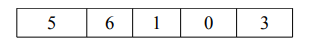
\includegraphics[keepaspectratio]{images/ejemplo.png}}

Implementaremos el metodo de burbuja para poder resolver nuestro
problema

\begin{Shaded}
\begin{Highlighting}[]
\KeywordTok{public} \KeywordTok{class}\NormalTok{ Ejemplo }\OperatorTok{\{}

    \KeywordTok{public} \DataTypeTok{static} \DataTypeTok{void} \FunctionTok{main}\OperatorTok{(}\BuiltInTok{String}\OperatorTok{[]}\NormalTok{ args}\OperatorTok{)} \OperatorTok{\{}
        \DataTypeTok{int}\NormalTok{ nums}\OperatorTok{[]} \OperatorTok{=} \OperatorTok{\{}\DecValTok{5}\OperatorTok{,} \DecValTok{6}\OperatorTok{,} \DecValTok{1}\OperatorTok{,} \DecValTok{0}\OperatorTok{,} \DecValTok{3}\OperatorTok{\};}
        \DataTypeTok{int}\NormalTok{ size }\OperatorTok{=}\NormalTok{ nums}\OperatorTok{.}\FunctionTok{length}\OperatorTok{;}
        \DataTypeTok{int}\NormalTok{ temp }\OperatorTok{=} \DecValTok{0}\OperatorTok{;}
        \ControlFlowTok{for} \OperatorTok{(}\DataTypeTok{int}\NormalTok{ i }\OperatorTok{=} \DecValTok{0}\OperatorTok{;}\NormalTok{ i }\OperatorTok{\textless{}}\NormalTok{ size}\OperatorTok{;}\NormalTok{ i}\OperatorTok{++)} \OperatorTok{\{}
            \ControlFlowTok{for} \OperatorTok{(}\DataTypeTok{int}\NormalTok{ j }\OperatorTok{=} \DecValTok{0}\OperatorTok{;}\NormalTok{ j }\OperatorTok{\textless{}}\NormalTok{ size }\OperatorTok{{-}}\NormalTok{ i }\OperatorTok{{-}} \DecValTok{1}\OperatorTok{;}\NormalTok{ j}\OperatorTok{++)} \OperatorTok{\{}
                \ControlFlowTok{if} \OperatorTok{(}\NormalTok{nums}\OperatorTok{[}\NormalTok{j}\OperatorTok{]} \OperatorTok{\textgreater{}}\NormalTok{ nums}\OperatorTok{[}\NormalTok{j }\OperatorTok{+} \DecValTok{1}\OperatorTok{])} \OperatorTok{\{}
\NormalTok{                    temp }\OperatorTok{=}\NormalTok{ nums}\OperatorTok{[}\NormalTok{j}\OperatorTok{];}
\NormalTok{                    nums}\OperatorTok{[}\NormalTok{j}\OperatorTok{]} \OperatorTok{=}\NormalTok{ nums}\OperatorTok{[}\NormalTok{j }\OperatorTok{+} \DecValTok{1}\OperatorTok{];}
\NormalTok{                    nums}\OperatorTok{[}\NormalTok{j }\OperatorTok{+} \DecValTok{1}\OperatorTok{]} \OperatorTok{=}\NormalTok{ temp}\OperatorTok{;}
                \OperatorTok{\}}
            \OperatorTok{\}}
        \OperatorTok{\}}
        \ControlFlowTok{for} \OperatorTok{(}\DataTypeTok{int}\NormalTok{ num }\OperatorTok{:}\NormalTok{ nums}\OperatorTok{)} \OperatorTok{\{}

            \BuiltInTok{System}\OperatorTok{.}\FunctionTok{out}\OperatorTok{.}\FunctionTok{print}\OperatorTok{(}\NormalTok{num }\OperatorTok{+} \StringTok{" "} \OperatorTok{);}

        \OperatorTok{\}}

    \OperatorTok{\}}
\OperatorTok{\}}
\end{Highlighting}
\end{Shaded}

Como nos pide que ordenemos de menor a mayor nuestra funcion comparara
todos los valores de izquierda a derecha comenzando por el número 5,
después con el 6, el 1, el 0 y el 3, si el número actual es mayor que el
de su derecha intercambiara su posición con su vecino y seguira asi en
bucle hasta que los valores de su derecha no sean mayores que los de su
izquierda, dandonos como resultado sus valores ordenados

\pandocbounded{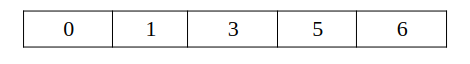
\includegraphics[keepaspectratio]{images/correcto.png}}

\subsection{Implementación en Python}\label{implementaciuxf3n-en-python}

\begin{Shaded}
\begin{Highlighting}[]
\NormalTok{nums }\OperatorTok{=}\NormalTok{ [}\DecValTok{5}\NormalTok{, }\DecValTok{6}\NormalTok{, }\DecValTok{1}\NormalTok{, }\DecValTok{0}\NormalTok{, }\DecValTok{3}\NormalTok{]}
\NormalTok{size }\OperatorTok{=} \BuiltInTok{len}\NormalTok{(nums)}

\ControlFlowTok{for}\NormalTok{ i }\KeywordTok{in} \BuiltInTok{range}\NormalTok{(size):}
    \ControlFlowTok{for}\NormalTok{ j }\KeywordTok{in} \BuiltInTok{range}\NormalTok{(}\DecValTok{0}\NormalTok{, size }\OperatorTok{{-}}\NormalTok{ i }\OperatorTok{{-}} \DecValTok{1}\NormalTok{):}
        \ControlFlowTok{if}\NormalTok{ nums[j] }\OperatorTok{\textgreater{}}\NormalTok{ nums[j }\OperatorTok{+} \DecValTok{1}\NormalTok{]:}
\NormalTok{            nums[j], nums[j }\OperatorTok{+} \DecValTok{1}\NormalTok{] }\OperatorTok{=}\NormalTok{ nums[j }\OperatorTok{+} \DecValTok{1}\NormalTok{], nums[j]}


\ControlFlowTok{for}\NormalTok{ num }\KeywordTok{in}\NormalTok{ nums:}
    \BuiltInTok{print}\NormalTok{(num, end}\OperatorTok{=}\StringTok{" "}\NormalTok{)}
    
\end{Highlighting}
\end{Shaded}

\subsection{Implementación en
JavaScript}\label{implementaciuxf3n-en-javascript}

\begin{Shaded}
\begin{Highlighting}[]
\KeywordTok{let}\NormalTok{ nums }\OperatorTok{=}\NormalTok{ [}\DecValTok{5}\OperatorTok{,} \DecValTok{6}\OperatorTok{,} \DecValTok{1}\OperatorTok{,} \DecValTok{0}\OperatorTok{,} \DecValTok{3}\NormalTok{]}\OperatorTok{;}
\KeywordTok{let}\NormalTok{ size }\OperatorTok{=}\NormalTok{ nums}\OperatorTok{.}\AttributeTok{length}\OperatorTok{;}
\KeywordTok{let}\NormalTok{ temp }\OperatorTok{=} \DecValTok{0}\OperatorTok{;}

\ControlFlowTok{for}\NormalTok{ (}\KeywordTok{let}\NormalTok{ i }\OperatorTok{=} \DecValTok{0}\OperatorTok{;}\NormalTok{ i }\OperatorTok{\textless{}}\NormalTok{ size}\OperatorTok{;}\NormalTok{ i}\OperatorTok{++}\NormalTok{) \{}
    \ControlFlowTok{for}\NormalTok{ (}\KeywordTok{let}\NormalTok{ j }\OperatorTok{=} \DecValTok{0}\OperatorTok{;}\NormalTok{ j }\OperatorTok{\textless{}}\NormalTok{ size }\OperatorTok{{-}}\NormalTok{ i }\OperatorTok{{-}} \DecValTok{1}\OperatorTok{;}\NormalTok{ j}\OperatorTok{++}\NormalTok{) \{}
        \ControlFlowTok{if}\NormalTok{ (nums[j] }\OperatorTok{\textgreater{}}\NormalTok{ nums[j }\OperatorTok{+} \DecValTok{1}\NormalTok{]) \{}
\NormalTok{            temp }\OperatorTok{=}\NormalTok{ nums[j]}\OperatorTok{;}
\NormalTok{            nums[j] }\OperatorTok{=}\NormalTok{ nums[j }\OperatorTok{+} \DecValTok{1}\NormalTok{]}\OperatorTok{;}
\NormalTok{            nums[j }\OperatorTok{+} \DecValTok{1}\NormalTok{] }\OperatorTok{=}\NormalTok{ temp}\OperatorTok{;}
\NormalTok{        \}}
\NormalTok{    \}}
\NormalTok{\}}

\BuiltInTok{console}\OperatorTok{.}\FunctionTok{log}\NormalTok{(nums}\OperatorTok{.}\FunctionTok{join}\NormalTok{(}\StringTok{" "}\NormalTok{))}\OperatorTok{;}
\end{Highlighting}
\end{Shaded}

\section{\texorpdfstring{\textbf{Insertion
Sort}}{Insertion Sort}}\label{insertion-sort}

\subsection{\texorpdfstring{\textbf{Concepto}}{Concepto}}\label{concepto-1}

El \textbf{Insertion Sort} (ordenación por inserción) es un algoritmo de
ordenamiento simple diseñado para procesar una cantidad pequeña de
elementos. Su funcionamiento técnico consiste en recorrer un arreglo
desde el segundo elemento (índice 1) y compararlo, tratándolo como una
``clave'' (key), con los elementos precedentes. Si los elementos
anteriores son mayores que la clave, el algoritmo los desplaza una
posición hacia adelante para permitir la inserción del valor clave en su
lugar correspondiente. Se clasifica como un algoritmo de comparación
\textbf{no recursivo}, \textbf{estable} (mantiene el orden de elementos
con claves iguales) y \textbf{en el lugar} (in-place), lo que significa
que no requiere memoria adicional significativa para su ejecución. En
términos de rendimiento práctico, es superior al Bubble Sort, siendo
hasta 5 veces más rápido en implementaciones en Java({freeCodeCamp.org}
2023).

En este capítulo, exploraremos algunos de los algoritmos de ordenación
más conocidos y fundamentales: Burbuja (Bubble Sort), Inserción
(Insertion Sort), Mergesort y Quicksort. Analizaremos su funcionamiento,
implementaremos cada uno en R con bloques de código ejecutables y
discutiremos sus características de rendimiento, incluyendo su
complejidad temporal y espacial.

\subsection{\texorpdfstring{\textbf{Codigo en
java}}{Codigo en java}}\label{codigo-en-java}

\begin{Shaded}
\begin{Highlighting}[]
\KeywordTok{public} \DataTypeTok{static} \DataTypeTok{void} \FunctionTok{insertionSort}\OperatorTok{(}\DataTypeTok{int}\OperatorTok{[]}\NormalTok{ arr}\OperatorTok{)} \OperatorTok{\{}
    \DataTypeTok{int}\NormalTok{ n }\OperatorTok{=}\NormalTok{ arr}\OperatorTok{.}\FunctionTok{length}\OperatorTok{;}
    \ControlFlowTok{for} \OperatorTok{(}\DataTypeTok{int}\NormalTok{ i }\OperatorTok{=} \DecValTok{1}\OperatorTok{;}\NormalTok{ i }\OperatorTok{\textless{}}\NormalTok{ n}\OperatorTok{;}\NormalTok{ i}\OperatorTok{++)} \OperatorTok{\{}
        \DataTypeTok{int}\NormalTok{ key }\OperatorTok{=}\NormalTok{ arr}\OperatorTok{[}\NormalTok{i}\OperatorTok{];}
        \DataTypeTok{int}\NormalTok{ j }\OperatorTok{=}\NormalTok{ i }\OperatorTok{{-}} \DecValTok{1}\OperatorTok{;}
        \ControlFlowTok{while} \OperatorTok{(}\NormalTok{j }\OperatorTok{\textgreater{}=} \DecValTok{0} \OperatorTok{\&\&}\NormalTok{ arr}\OperatorTok{[}\NormalTok{j}\OperatorTok{]} \OperatorTok{\textgreater{}}\NormalTok{ key}\OperatorTok{)} \OperatorTok{\{}
\NormalTok{            arr}\OperatorTok{[}\NormalTok{j }\OperatorTok{+} \DecValTok{1}\OperatorTok{]} \OperatorTok{=}\NormalTok{ arr}\OperatorTok{[}\NormalTok{j}\OperatorTok{];}
\NormalTok{            j }\OperatorTok{=}\NormalTok{ j }\OperatorTok{{-}} \DecValTok{1}\OperatorTok{;}
        \OperatorTok{\}}
\NormalTok{        arr}\OperatorTok{[}\NormalTok{j }\OperatorTok{+} \DecValTok{1}\OperatorTok{]} \OperatorTok{=}\NormalTok{ key}\OperatorTok{;}
    \OperatorTok{\}}
\OperatorTok{\}}
\end{Highlighting}
\end{Shaded}

\subsubsection{\texorpdfstring{\textbf{Explicacion del
codigo}}{Explicacion del codigo}}\label{explicacion-del-codigo}

El procedimiento inicia la iteración en el índice 1 del arreglo. El
valor en la posición actual se almacena en la variable \texttt{key}. Un
bucle interno retrocede por los elementos anteriores (índice
\texttt{j}); mientras estos sean mayores que la clave, se desplazan una
posición a la derecha. Finalmente, la clave se inserta en la posición
vacía generada.

\subsubsection{\texorpdfstring{\textbf{complejidad del
algoritmo}}{complejidad del algoritmo}}\label{complejidad-del-algoritmo}

\begin{itemize}
\tightlist
\item
  \textbf{Temporal (Peor y promedio):} \(O(n^2)\), ocurre cuando el
  arreglo está ordenado de forma inversa o aleatoria.
\item
  \textbf{Temporal (Mejor caso):} \(O(n)\), sucede cuando el arreglo ya
  se encuentra ordenado, requiriendo solo una pasada.
\item
  \textbf{Espacial:} \(O(1)\), ya que las operaciones de ordenamiento se
  ejecutan directamente sobre el arreglo original (in-place).
\end{itemize}

\subsubsection{\texorpdfstring{\textbf{Ejemplo}}{Ejemplo}}\label{ejemplo-1}

Dado el arreglo inicial :

\begin{enumerate}
\def\labelenumi{\arabic{enumi}.}
\tightlist
\item
  \textbf{Paso 1:} Clave = 3. Como \(8 > 3\), el 8 se mueve a la
  derecha.
\item
  \textbf{Paso 2:} Clave = 5. Como \(8 > 5\), el 8 se mueve a la
  derecha.
\item
  \textbf{Paso 3:} Clave = 1. Se desplazan consecutivamente 8, 5 y 3
  para insertar el 1 al inicio.
\end{enumerate}

El algoritmo de ordenación por burbuja es uno de los más sencillos de
entender e implementar. Su nombre proviene del hecho de que los
elementos más ``grandes'' (o más ``pesados'', si imaginamos burbujas)
``flotan'' gradualmente hacia el final de la lista a medida que se
realizan comparaciones y posibles intercambios.

\subsection{\texorpdfstring{\textbf{Código en
python}}{Código en python}}\label{cuxf3digo-en-python}

\begin{Shaded}
\begin{Highlighting}[]
\KeywordTok{def}\NormalTok{ insertion\_sort(arr):}
    \ControlFlowTok{for}\NormalTok{ i }\KeywordTok{in} \BuiltInTok{range}\NormalTok{(}\DecValTok{1}\NormalTok{, }\BuiltInTok{len}\NormalTok{(arr)):}
\NormalTok{        key }\OperatorTok{=}\NormalTok{ arr[i]}
\NormalTok{        j }\OperatorTok{=}\NormalTok{ i }\OperatorTok{{-}} \DecValTok{1}
        \ControlFlowTok{while}\NormalTok{ j }\OperatorTok{\textgreater{}=} \DecValTok{0} \KeywordTok{and}\NormalTok{ key }\OperatorTok{\textless{}}\NormalTok{ arr[j]:}
\NormalTok{            arr[j }\OperatorTok{+} \DecValTok{1}\NormalTok{] }\OperatorTok{=}\NormalTok{ arr[j]}
\NormalTok{            j }\OperatorTok{{-}=} \DecValTok{1}
\NormalTok{        arr[j }\OperatorTok{+} \DecValTok{1}\NormalTok{] }\OperatorTok{=}\NormalTok{ key}
\end{Highlighting}
\end{Shaded}

\subsubsection{\texorpdfstring{\textbf{Explicacion del
codigo}}{Explicacion del codigo}}\label{explicacion-del-codigo-1}

La implementación en Python utiliza un ciclo \texttt{for} para recorrer
la lista y un ciclo \texttt{while} para realizar los desplazamientos
necesarios hacia la derecha. Esta técnica es fundamental en algoritmos
modernos como el \textbf{Timsort}, que es una mezcla de Insertion Sort y
Merge Sort utilizada por defecto en las funciones de ordenamiento
nativas de Python.

\subsubsection{\texorpdfstring{\textbf{complejidad del
algoritmo}}{complejidad del algoritmo}}\label{complejidad-del-algoritmo-1}

Mantiene una complejidad temporal de \textbf{\(O(n^2)\)} en casos
desfavorables. Es un algoritmo \textbf{estable}, garantizando que no se
altere el orden relativo de elementos que posean valores idénticos.

\subsubsection{\texorpdfstring{\textbf{Ejemplo}}{Ejemplo}}\label{ejemplo-2}

En una lista, al procesar la clave 5:

\begin{enumerate}
\def\labelenumi{\arabic{enumi}.}
\tightlist
\item
  Se compara 5 con 8. Dado que \(8 > 5\), el 8 se desplaza.
\item
  Se compara 5 con 4. Dado que \(4 < 5\), el desplazamiento se detiene y
  el 5 se inserta en la posición inmediatamente posterior al 4.
\end{enumerate}

\subsection{\texorpdfstring{\textbf{Codigo en
javascript}}{Codigo en javascript}}\label{codigo-en-javascript}

\begin{Shaded}
\begin{Highlighting}[]
\KeywordTok{function} \FunctionTok{insertionSort}\NormalTok{(arr) \{}
  \ControlFlowTok{for}\NormalTok{ (}\KeywordTok{let}\NormalTok{ i }\OperatorTok{=} \DecValTok{1}\OperatorTok{;}\NormalTok{ i }\OperatorTok{\textless{}}\NormalTok{ arr}\OperatorTok{.}\AttributeTok{length}\OperatorTok{;}\NormalTok{ i}\OperatorTok{++}\NormalTok{) \{}
    \KeywordTok{let}\NormalTok{ key }\OperatorTok{=}\NormalTok{ arr[i]}\OperatorTok{;}
    \KeywordTok{let}\NormalTok{ j }\OperatorTok{=}\NormalTok{ i }\OperatorTok{{-}} \DecValTok{1}\OperatorTok{;}
    \ControlFlowTok{while}\NormalTok{ (j }\OperatorTok{\textgreater{}=} \DecValTok{0} \OperatorTok{\&\&}\NormalTok{ arr[j] }\OperatorTok{\textgreater{}}\NormalTok{ key) \{}
\NormalTok{      arr[j }\OperatorTok{+} \DecValTok{1}\NormalTok{] }\OperatorTok{=}\NormalTok{ arr[j]}\OperatorTok{;}
\NormalTok{      j}\OperatorTok{{-}{-};}
\NormalTok{    \}}
\NormalTok{    arr[j }\OperatorTok{+} \DecValTok{1}\NormalTok{] }\OperatorTok{=}\NormalTok{ key}\OperatorTok{;}
\NormalTok{  \}}
  \ControlFlowTok{return}\NormalTok{ arr}\OperatorTok{;}
\NormalTok{\}}
\end{Highlighting}
\end{Shaded}

\subsubsection{\texorpdfstring{\textbf{Explicacion del
codigo}}{Explicacion del codigo}}\label{explicacion-del-codigo-2}

El algoritmo itera desde la segunda posición del arreglo, extrayendo el
elemento clave y comparándolo de forma regresiva con los elementos ya
procesados a su izquierda. Los elementos se desplazan hacia la derecha
hasta localizar el punto de inserción exacto para la clave.

\subsubsection{\texorpdfstring{\textbf{complejidad del
algoritmo}}{complejidad del algoritmo}}\label{complejidad-del-algoritmo-2}

La complejidad temporal promedio es \textbf{\(O(n^2)\)}, lo que lo hace
menos eficiente para grandes conjuntos de datos en comparación con
algoritmos de orden \(O(n \log n)\). No obstante, su bajo consumo de
recursos (espacio \textbf{\(O(1)\)}) lo hace adecuado para sistemas con
limitaciones de memoria.

\subsubsection{\texorpdfstring{\textbf{Ejemplo}}{Ejemplo}}\label{ejemplo-3}

Con el arreglo:

\begin{enumerate}
\def\labelenumi{\arabic{enumi}.}
\tightlist
\item
  La clave 1 se compara con 6, 4, 3 y 2 consecutivamente.
\item
  Cada uno de estos elementos se desplaza un lugar a la derecha.
\item
  El 1 se inserta en el índice 0, resultando en la lista final
  ordenada:.
\end{enumerate}

\section{Merge Sort}\label{merge-sort}

\subsection{Concepto}\label{concepto-2}

Merge Sort es un algoritmo de ordenamiento avanzado quee se base en el
pricipio de ``Divide y Vencerás'', utilizado con frecuencia para
sistemas que requieren alto redimiento, estabilidad y eficiencia al
trabajar con grandes volúmenes de datos.(Ası́n 2021) Su principal ventaja
es mantener un tiempo de ejcucion predecibles incluso cuando el tamaño
de los datos aumenta. El funcionamiento del Merge Sort consiste en
dividir de manera repetitiva un arreglo en partes mas pequeñas hasta
obtener subproblemas de un solo elemento que se lo considera
ordenado.(Gurin 2004) Posteriormente el argorroritmo empieza a mezclar
de manera ordenada comparando sus elementos hasta reconstruir
completamente el arreglo original, pero ahora organizado en orden
ascendente. Este proceso puede imaginarse como el ordenamiento de una
baraja de cartas. Si intentáramos ordenarla de manera tradicional,
tendríamos que revisar varias veces las mismas cartas para determinar su
posición correcta. Sin embargo, al aplicar el principio de ``Divide y
Vencerás'', la baraja puede dividirse en grupos más pequeños,
facilitando el ordenamiento de cada parte por separado. Permitiendo que
los grupos ya ordenados se vuelven a unir poco a poco hasta obtener toda
la baraja organizada.

\begin{figure}[H]

{\centering 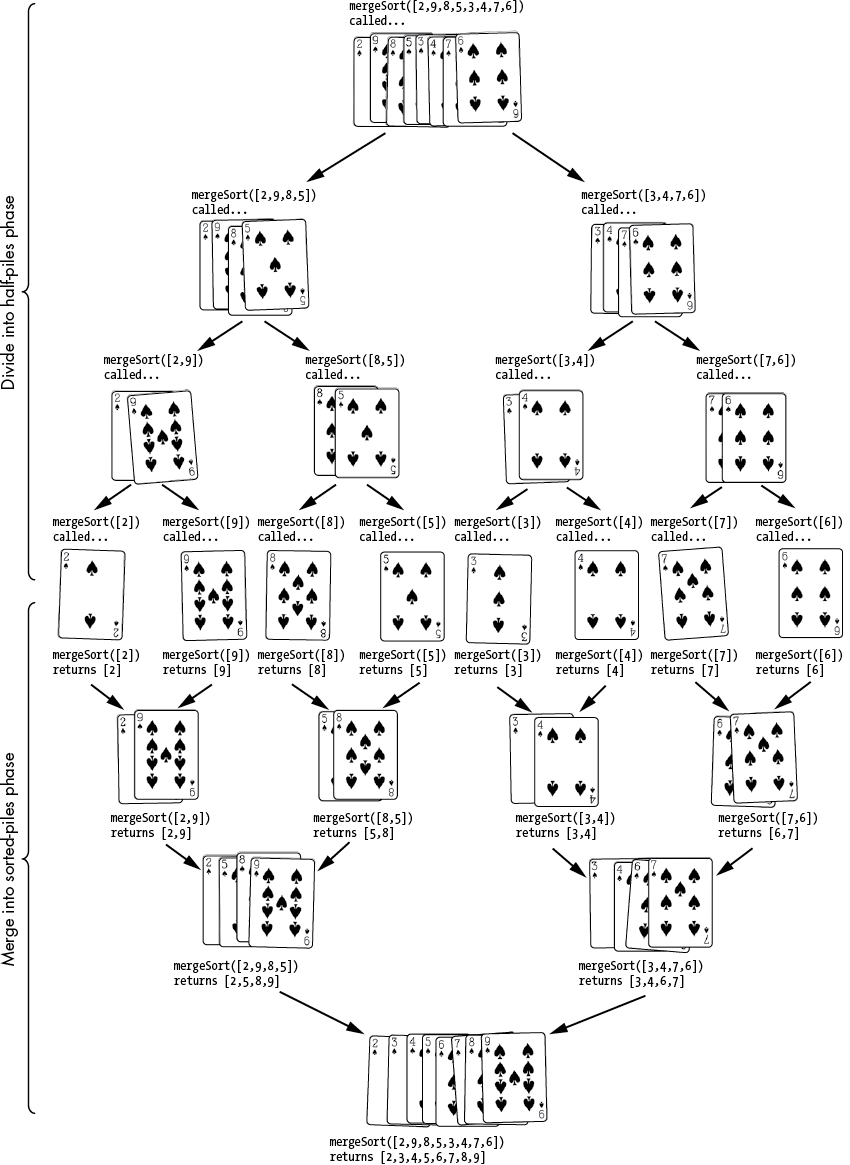
\includegraphics[width=0.7\linewidth,height=\textheight,keepaspectratio]{images/000059.jpg}

}

\caption{Cartas ordenadas mediante Merge Sort}

\end{figure}%

El algoritmo funciona siguiento tres pasos principales:

\begin{enumerate}
\def\labelenumi{\arabic{enumi}.}
\tightlist
\item
  \textbf{Dividir}: Si el arreglo contiene varios elemento este se
  divide a la mitad en dos subgrupos diferentes reduciendo el problema
  en partes mas pequeñas.
\item
  \textbf{Vencer}: Una vez divididos en subgrupos se aplica el mismo
  procesos de divicion de manera recursiva a cada subgrupo hasta obtener
  subarreglos de un solo elemento.
\item
  \textbf{Combinar (Merge)}: Finalmente todos los subarreglos se unen de
  forma ordenada comparando cada uno de sus elementos colocandolos en
  sus posicion correcta hasta formar un nuevo super arreglo.
\end{enumerate}

Este proceso continúa ejecutándose de manera recursiva hasta llegar a
subarreglos de un solo elemento. Debido a que cada subarreglo contiene
únicamente un dato, estos se consideran ordenados. A partir de ese
punto, el algoritmo comienza el proceso de mezcla y reconstrucción
ordenada hasta obtener el arreglo final completamente organizado.

\subsection[Implementación en Java \hfill
]{\texorpdfstring{Implementación en Java
\protect
\includegraphics[width=0.1\linewidth,height=\textheight,keepaspectratio]{images/p-80-java.png}\hfill
}{Implementación en Java }}\label{implementaciuxf3n-en-java-1}

Para la realizacion de este algoritmo necesitaremos dos funciones: una
para la lógica recursiva de división (\texttt{merge\_sort}) y otra para
la combinación de dos arrays ya ordenados (\texttt{merge\_arrays}).

\begin{Shaded}
\begin{Highlighting}[]
\CommentTok{//| eval: false}
\KeywordTok{public} \KeywordTok{class}\NormalTok{ Mergesort }\OperatorTok{\{}
    \CommentTok{/*}
\CommentTok{     * Metodo encargado de combinar dos subarreglos ordenados}
\CommentTok{     * en un unico arreglo ordenado.}
\CommentTok{     */}
    \KeywordTok{public} \DataTypeTok{void} \FunctionTok{merge\_arrays}\OperatorTok{(}\DataTypeTok{int}\OperatorTok{[]}\NormalTok{ arr}\OperatorTok{,} \DataTypeTok{int}\NormalTok{ l}\OperatorTok{,} \DataTypeTok{int}\NormalTok{ m}\OperatorTok{,} \DataTypeTok{int}\NormalTok{ r}\OperatorTok{)} \OperatorTok{\{}

        \CommentTok{// Tamaño del subarreglo izquierdo}
        \DataTypeTok{int}\NormalTok{ n1 }\OperatorTok{=}\NormalTok{ m }\OperatorTok{{-}}\NormalTok{ l }\OperatorTok{+} \DecValTok{1}\OperatorTok{;}

        \CommentTok{// Tamaño del subarreglo derecho}
        \DataTypeTok{int}\NormalTok{ n2 }\OperatorTok{=}\NormalTok{ r }\OperatorTok{{-}}\NormalTok{ m}\OperatorTok{;}

        \CommentTok{// Arreglos auxiliares}
        \DataTypeTok{int}\OperatorTok{[]}\NormalTok{ L }\OperatorTok{=} \KeywordTok{new} \DataTypeTok{int}\OperatorTok{[}\NormalTok{n1}\OperatorTok{];}
        \DataTypeTok{int}\OperatorTok{[]}\NormalTok{ R }\OperatorTok{=} \KeywordTok{new} \DataTypeTok{int}\OperatorTok{[}\NormalTok{n2}\OperatorTok{];}

        \CommentTok{// Copiar elementos al arreglo izquierdo}
        \ControlFlowTok{for} \OperatorTok{(}\DataTypeTok{int}\NormalTok{ i }\OperatorTok{=} \DecValTok{0}\OperatorTok{;}\NormalTok{ i }\OperatorTok{\textless{}}\NormalTok{ n1}\OperatorTok{;}\NormalTok{ i}\OperatorTok{++)} \OperatorTok{\{}
\NormalTok{            L}\OperatorTok{[}\NormalTok{i}\OperatorTok{]} \OperatorTok{=}\NormalTok{ arr}\OperatorTok{[}\NormalTok{l }\OperatorTok{+}\NormalTok{ i}\OperatorTok{];}
        \OperatorTok{\}}

        \CommentTok{// Copiar elementos al arreglo derecho}
        \ControlFlowTok{for} \OperatorTok{(}\DataTypeTok{int}\NormalTok{ j }\OperatorTok{=} \DecValTok{0}\OperatorTok{;}\NormalTok{ j }\OperatorTok{\textless{}}\NormalTok{ n2}\OperatorTok{;}\NormalTok{ j}\OperatorTok{++)} \OperatorTok{\{}
\NormalTok{            R}\OperatorTok{[}\NormalTok{j}\OperatorTok{]} \OperatorTok{=}\NormalTok{ arr}\OperatorTok{[}\NormalTok{m }\OperatorTok{+} \DecValTok{1} \OperatorTok{+}\NormalTok{ j}\OperatorTok{];}
        \OperatorTok{\}}

        \CommentTok{// Variables de control}
        \DataTypeTok{int}\NormalTok{ i }\OperatorTok{=} \DecValTok{0}\OperatorTok{;} \CommentTok{// Indice del arreglo izquierdo}
        \DataTypeTok{int}\NormalTok{ j }\OperatorTok{=} \DecValTok{0}\OperatorTok{;} \CommentTok{// Indice del arreglo derecho}
        \DataTypeTok{int}\NormalTok{ k }\OperatorTok{=}\NormalTok{ l}\OperatorTok{;} \CommentTok{// Indice del arreglo principal}


        \CommentTok{//Comparar elementos de ambos arreglos y colocarlos en orden ascendente}
        \ControlFlowTok{while} \OperatorTok{(}\NormalTok{i }\OperatorTok{\textless{}}\NormalTok{ n1 }\OperatorTok{\&\&}\NormalTok{ j }\OperatorTok{\textless{}}\NormalTok{ n2}\OperatorTok{)} \OperatorTok{\{}
            \ControlFlowTok{if} \OperatorTok{(}\NormalTok{L}\OperatorTok{[}\NormalTok{i}\OperatorTok{]} \OperatorTok{\textless{}=}\NormalTok{ R}\OperatorTok{[}\NormalTok{j}\OperatorTok{])} \OperatorTok{\{}
\NormalTok{                arr}\OperatorTok{[}\NormalTok{k}\OperatorTok{]} \OperatorTok{=}\NormalTok{ L}\OperatorTok{[}\NormalTok{i}\OperatorTok{];}
\NormalTok{                i}\OperatorTok{++;}
            \OperatorTok{\}} \ControlFlowTok{else} \OperatorTok{\{}
\NormalTok{                arr}\OperatorTok{[}\NormalTok{k}\OperatorTok{]} \OperatorTok{=}\NormalTok{ R}\OperatorTok{[}\NormalTok{j}\OperatorTok{];}
\NormalTok{                j}\OperatorTok{++;}
            \OperatorTok{\}}
\NormalTok{            k}\OperatorTok{++;}
        \OperatorTok{\}}

        \CommentTok{//Copiar los elementos restantes del arreglo izquierdo}
        \ControlFlowTok{while} \OperatorTok{(}\NormalTok{i }\OperatorTok{\textless{}}\NormalTok{ n1}\OperatorTok{)} \OperatorTok{\{}
\NormalTok{            arr}\OperatorTok{[}\NormalTok{k}\OperatorTok{]} \OperatorTok{=}\NormalTok{ L}\OperatorTok{[}\NormalTok{i}\OperatorTok{];}
\NormalTok{            i}\OperatorTok{++;}
\NormalTok{            k}\OperatorTok{++;}
        \OperatorTok{\}}
        \CommentTok{//Copiar los elementos restantes del arreglo derecho}
        \ControlFlowTok{while} \OperatorTok{(}\NormalTok{j }\OperatorTok{\textless{}}\NormalTok{ n2}\OperatorTok{)} \OperatorTok{\{}
\NormalTok{            arr}\OperatorTok{[}\NormalTok{k}\OperatorTok{]} \OperatorTok{=}\NormalTok{ R}\OperatorTok{[}\NormalTok{j}\OperatorTok{];}
\NormalTok{            j}\OperatorTok{++;}
\NormalTok{            k}\OperatorTok{++;}
        \OperatorTok{\}}
    \OperatorTok{\}}

    \CommentTok{/*}
\CommentTok{     * Metodo principal de Merge Sort.}
\CommentTok{     * Divide el arreglo recursivamente.}
\CommentTok{     */}
    \KeywordTok{public} \DataTypeTok{void} \FunctionTok{merge\_sort}\OperatorTok{(}\DataTypeTok{int}\NormalTok{ arr}\OperatorTok{[],} \DataTypeTok{int}\NormalTok{ l}\OperatorTok{,} \DataTypeTok{int}\NormalTok{ r}\OperatorTok{)} \OperatorTok{\{}
        \ControlFlowTok{if} \OperatorTok{(}\NormalTok{l }\OperatorTok{\textless{}}\NormalTok{ r}\OperatorTok{)} \OperatorTok{\{}
          
            \CommentTok{// Calculo del punto medio}
            \DataTypeTok{int}\NormalTok{ m }\OperatorTok{=}\NormalTok{ l }\OperatorTok{+} \OperatorTok{(}\NormalTok{r }\OperatorTok{{-}}\NormalTok{ l}\OperatorTok{)} \OperatorTok{/} \DecValTok{2}\OperatorTok{;}
            
            \CommentTok{// Ordenar mitad izquierda}
            \FunctionTok{merge\_sort}\OperatorTok{(}\NormalTok{arr}\OperatorTok{,}\NormalTok{ l}\OperatorTok{,}\NormalTok{ m}\OperatorTok{);}
            
            \CommentTok{// Ordenar mitad derecha}
            \FunctionTok{merge\_sort}\OperatorTok{(}\NormalTok{arr}\OperatorTok{,}\NormalTok{ m }\OperatorTok{+} \DecValTok{1}\OperatorTok{,}\NormalTok{ r}\OperatorTok{);}
            
            \CommentTok{// Combinar ambas mitades}
            \FunctionTok{merge\_arrays}\OperatorTok{(}\NormalTok{arr}\OperatorTok{,}\NormalTok{ l}\OperatorTok{,}\NormalTok{ m}\OperatorTok{,}\NormalTok{ r}\OperatorTok{);}
        \OperatorTok{\}}
    \OperatorTok{\}}
\OperatorTok{\}}
\end{Highlighting}
\end{Shaded}

\subsection[Implementación en Python \hfill
]{\texorpdfstring{Implementación en Python
\protect
\includegraphics[width=0.1\linewidth,height=\textheight,keepaspectratio]{images/Python-Emblem.png}\hfill
}{Implementación en Python }}\label{implementaciuxf3n-en-python-1}

\begin{Shaded}
\begin{Highlighting}[]
\CommentTok{\#| eval: false}
\KeywordTok{class}\NormalTok{ Mergesort:}
    \CommentTok{\# Metodo encargado de combinar dos subarreglos ordenados en un unico arreglo ordenado.}
    \KeywordTok{def}\NormalTok{ merge\_arrays(}\VariableTok{self}\NormalTok{, arr, l, m, r):}

        \CommentTok{\# Tamaño del subarreglo izquierdo}
\NormalTok{        n1 }\OperatorTok{=}\NormalTok{ m }\OperatorTok{{-}}\NormalTok{ l }\OperatorTok{+} \DecValTok{1}

        \CommentTok{\# Tamaño del subarreglo derecho}
\NormalTok{        n2 }\OperatorTok{=}\NormalTok{ r }\OperatorTok{{-}}\NormalTok{ m}

        \CommentTok{\# Arreglos auxiliares}
\NormalTok{        L }\OperatorTok{=}\NormalTok{ [}\DecValTok{0}\NormalTok{] }\OperatorTok{*}\NormalTok{ n1}
\NormalTok{        R }\OperatorTok{=}\NormalTok{ [}\DecValTok{0}\NormalTok{] }\OperatorTok{*}\NormalTok{ n2}

        \CommentTok{\# Copiar elementos al arreglo izquierdo}
        \ControlFlowTok{for}\NormalTok{ i }\KeywordTok{in} \BuiltInTok{range}\NormalTok{(n1):}
\NormalTok{            L[i] }\OperatorTok{=}\NormalTok{ arr[l }\OperatorTok{+}\NormalTok{ i]}

        \CommentTok{\# Copiar elementos al arreglo derecho}
        \ControlFlowTok{for}\NormalTok{ j }\KeywordTok{in} \BuiltInTok{range}\NormalTok{(n2):}
\NormalTok{            R[j] }\OperatorTok{=}\NormalTok{ arr[m }\OperatorTok{+} \DecValTok{1} \OperatorTok{+}\NormalTok{ j]}

        \CommentTok{\# Variables de control}
\NormalTok{        i }\OperatorTok{=} \DecValTok{0}   \CommentTok{\# Indice del arreglo izquierdo}
\NormalTok{        j }\OperatorTok{=} \DecValTok{0}   \CommentTok{\# Indice del arreglo derecho}
\NormalTok{        k }\OperatorTok{=}\NormalTok{ l   }\CommentTok{\# Indice del arreglo principal}
        
        \CommentTok{\#Comparar elementos de ambos arreglos y colocarlos en orden ascendente}
        \ControlFlowTok{while}\NormalTok{ i }\OperatorTok{\textless{}}\NormalTok{ n1 }\KeywordTok{and}\NormalTok{ j }\OperatorTok{\textless{}}\NormalTok{ n2:}
            \ControlFlowTok{if}\NormalTok{ L[i] }\OperatorTok{\textless{}=}\NormalTok{ R[j]:}
\NormalTok{                arr[k] }\OperatorTok{=}\NormalTok{ L[i]}
\NormalTok{                i }\OperatorTok{+=} \DecValTok{1}
            \ControlFlowTok{else}\NormalTok{:}
\NormalTok{                arr[k] }\OperatorTok{=}\NormalTok{ R[j]}
\NormalTok{                j }\OperatorTok{+=} \DecValTok{1}
\NormalTok{            k }\OperatorTok{+=} \DecValTok{1}
        
        \CommentTok{\#Copiar los elementos restantes del arreglo izquierdo}
        \ControlFlowTok{while}\NormalTok{ i }\OperatorTok{\textless{}}\NormalTok{ n1:}
\NormalTok{            arr[k] }\OperatorTok{=}\NormalTok{ L[i]}
\NormalTok{            i }\OperatorTok{+=} \DecValTok{1}
\NormalTok{            k }\OperatorTok{+=} \DecValTok{1}
        
        \CommentTok{\#Copiar los elementos restantes del arreglo derecho}
        \ControlFlowTok{while}\NormalTok{ j }\OperatorTok{\textless{}}\NormalTok{ n2:}
\NormalTok{            arr[k] }\OperatorTok{=}\NormalTok{ R[j]}
\NormalTok{            j }\OperatorTok{+=} \DecValTok{1}
\NormalTok{            k }\OperatorTok{+=} \DecValTok{1}

   
    \CommentTok{\# Metodo principal de Merge Sort Divide el arreglo recursivamente.}
    \KeywordTok{def}\NormalTok{ merge\_sort(}\VariableTok{self}\NormalTok{, arr, l, r):}

        \CommentTok{\# Verifica si el arreglo puede seguir dividiendose}
        \ControlFlowTok{if}\NormalTok{ l }\OperatorTok{\textless{}}\NormalTok{ r:}
            
            \CommentTok{\# Calculo del punto medio}
\NormalTok{            m }\OperatorTok{=}\NormalTok{ l }\OperatorTok{+}\NormalTok{ (r }\OperatorTok{{-}}\NormalTok{ l) }\OperatorTok{//} \DecValTok{2}
            
            \CommentTok{\# Ordenar mitad izquierda}
            \VariableTok{self}\NormalTok{.merge\_sort(arr, l, m)}
            
            \CommentTok{\# Ordenar mitad izquierda}
            \VariableTok{self}\NormalTok{.merge\_sort(arr, m }\OperatorTok{+} \DecValTok{1}\NormalTok{, r)}
            
            \CommentTok{\# Combinar ambas mitades}
            \VariableTok{self}\NormalTok{.merge\_arrays(arr, l, m, r)}
\end{Highlighting}
\end{Shaded}

\subsection[Implementación en JavaScript \hfill
]{\texorpdfstring{Implementación en JavaScript
\protect
\includegraphics[width=0.1\linewidth,height=\textheight,keepaspectratio]{images/javascript.png}\hfill
}{Implementación en JavaScript }}\label{implementaciuxf3n-en-javascript-1}

\begin{Shaded}
\begin{Highlighting}[]
\KeywordTok{class}\NormalTok{ MergeSort \{}

    \CommentTok{/*}
\CommentTok{     * Metodo encargado de combinar dos subarreglos ordenados}
\CommentTok{     * en un unico arreglo ordenado.}
\CommentTok{     */}
    \FunctionTok{merge\_arrays}\NormalTok{(arr}\OperatorTok{,}\NormalTok{ l}\OperatorTok{,}\NormalTok{ m}\OperatorTok{,}\NormalTok{ r) \{}

        \CommentTok{// Tamaño del subarreglo izquierdo}
        \KeywordTok{let}\NormalTok{ n1 }\OperatorTok{=}\NormalTok{ m }\OperatorTok{{-}}\NormalTok{ l }\OperatorTok{+} \DecValTok{1}\OperatorTok{;}

        \CommentTok{// Tamaño del subarreglo derecho}
        \KeywordTok{let}\NormalTok{ n2 }\OperatorTok{=}\NormalTok{ r }\OperatorTok{{-}}\NormalTok{ m}\OperatorTok{;}

        \CommentTok{// Arreglos auxiliares}
        \KeywordTok{let}\NormalTok{ L }\OperatorTok{=} \KeywordTok{new} \BuiltInTok{Array}\NormalTok{(n1)}\OperatorTok{;}
        \KeywordTok{let}\NormalTok{ R }\OperatorTok{=} \KeywordTok{new} \BuiltInTok{Array}\NormalTok{(n2)}\OperatorTok{;}

        \CommentTok{// Copiar elementos al arreglo izquierdo}
        \ControlFlowTok{for}\NormalTok{ (}\KeywordTok{let}\NormalTok{ i }\OperatorTok{=} \DecValTok{0}\OperatorTok{;}\NormalTok{ i }\OperatorTok{\textless{}}\NormalTok{ n1}\OperatorTok{;}\NormalTok{ i}\OperatorTok{++}\NormalTok{) \{}
\NormalTok{            L[i] }\OperatorTok{=}\NormalTok{ arr[l }\OperatorTok{+}\NormalTok{ i]}\OperatorTok{;}
\NormalTok{        \}}

        \CommentTok{// Copiar elementos al arreglo derecho}
        \ControlFlowTok{for}\NormalTok{ (}\KeywordTok{let}\NormalTok{ j }\OperatorTok{=} \DecValTok{0}\OperatorTok{;}\NormalTok{ j }\OperatorTok{\textless{}}\NormalTok{ n2}\OperatorTok{;}\NormalTok{ j}\OperatorTok{++}\NormalTok{) \{}
\NormalTok{            R[j] }\OperatorTok{=}\NormalTok{ arr[m }\OperatorTok{+} \DecValTok{1} \OperatorTok{+}\NormalTok{ j]}\OperatorTok{;}
\NormalTok{        \}}

        \CommentTok{// Variables de control}
        \KeywordTok{let}\NormalTok{ i }\OperatorTok{=} \DecValTok{0}\OperatorTok{;} \CommentTok{// Indice del arreglo izquierdo}
        \KeywordTok{let}\NormalTok{ j }\OperatorTok{=} \DecValTok{0}\OperatorTok{;} \CommentTok{// Indice del arreglo derecho}
        \KeywordTok{let}\NormalTok{ k }\OperatorTok{=}\NormalTok{ l}\OperatorTok{;} \CommentTok{// Indice del arreglo principal}

        \CommentTok{// Comparar elementos de ambos arreglos y colocarlos en orden ascendente}
        \ControlFlowTok{while}\NormalTok{ (i }\OperatorTok{\textless{}}\NormalTok{ n1 }\OperatorTok{\&\&}\NormalTok{ j }\OperatorTok{\textless{}}\NormalTok{ n2) \{}

            \ControlFlowTok{if}\NormalTok{ (L[i] }\OperatorTok{\textless{}=}\NormalTok{ R[j]) \{}
\NormalTok{                arr[k] }\OperatorTok{=}\NormalTok{ L[i]}\OperatorTok{;}
\NormalTok{                i}\OperatorTok{++;}

\NormalTok{            \} }\ControlFlowTok{else}\NormalTok{ \{}
\NormalTok{                arr[k] }\OperatorTok{=}\NormalTok{ R[j]}\OperatorTok{;}
\NormalTok{                j}\OperatorTok{++;}
\NormalTok{            \}}
\NormalTok{            k}\OperatorTok{++;}
\NormalTok{        \}}

        \CommentTok{// Copiar los elementos restantes del arreglo izquierdo}
        \ControlFlowTok{while}\NormalTok{ (i }\OperatorTok{\textless{}}\NormalTok{ n1) \{}
\NormalTok{            arr[k] }\OperatorTok{=}\NormalTok{ L[i]}\OperatorTok{;}
\NormalTok{            i}\OperatorTok{++;}
\NormalTok{            k}\OperatorTok{++;}
\NormalTok{        \}}

        \CommentTok{// Copiar los elementos restantes del arreglo derecho}
        \ControlFlowTok{while}\NormalTok{ (j }\OperatorTok{\textless{}}\NormalTok{ n2) \{}
\NormalTok{            arr[k] }\OperatorTok{=}\NormalTok{ R[j]}\OperatorTok{;}
\NormalTok{            j}\OperatorTok{++;}
\NormalTok{            k}\OperatorTok{++;}
\NormalTok{        \}}
\NormalTok{    \}}

    \CommentTok{/*}
\CommentTok{     * Metodo principal de Merge Sort.}
\CommentTok{     * Divide el arreglo recursivamente.}
\CommentTok{     */}
    \FunctionTok{merge\_sort}\NormalTok{(arr}\OperatorTok{,}\NormalTok{ l}\OperatorTok{,}\NormalTok{ r) \{}

        \ControlFlowTok{if}\NormalTok{ (l }\OperatorTok{\textless{}}\NormalTok{ r) \{}

            \CommentTok{// Calculo del punto medio}
            \KeywordTok{let}\NormalTok{ m }\OperatorTok{=}\NormalTok{ l }\OperatorTok{+} \BuiltInTok{Math}\OperatorTok{.}\FunctionTok{floor}\NormalTok{((r }\OperatorTok{{-}}\NormalTok{ l) }\OperatorTok{/} \DecValTok{2}\NormalTok{)}\OperatorTok{;}

            \CommentTok{// Ordenar mitad izquierda}
            \KeywordTok{this}\OperatorTok{.}\FunctionTok{merge\_sort}\NormalTok{(arr}\OperatorTok{,}\NormalTok{ l}\OperatorTok{,}\NormalTok{ m)}\OperatorTok{;}

            \CommentTok{// Ordenar mitad derecha}
            \KeywordTok{this}\OperatorTok{.}\FunctionTok{merge\_sort}\NormalTok{(arr}\OperatorTok{,}\NormalTok{ m }\OperatorTok{+} \DecValTok{1}\OperatorTok{,}\NormalTok{ r)}\OperatorTok{;}

            \CommentTok{// Combinar ambas mitades}
            \KeywordTok{this}\OperatorTok{.}\FunctionTok{merge\_arrays}\NormalTok{(arr}\OperatorTok{,}\NormalTok{ l}\OperatorTok{,}\NormalTok{ m}\OperatorTok{,}\NormalTok{ r)}\OperatorTok{;}
\NormalTok{        \}}
\NormalTok{    \}}
\end{Highlighting}
\end{Shaded}

\subsection{Explicación del Código
(Java)}\label{explicaciuxf3n-del-cuxf3digo-java-1}

\subsubsection{\texorpdfstring{\texttt{merge\_arrays(int{[}{]}\ arr,\ int\ l,\ int\ m,\ int\ r)}:}{merge\_arrays(int{[}{]} arr, int l, int m, int r):}}\label{merge_arraysint-arr-int-l-int-m-int-r}

\begin{enumerate}
\def\labelenumi{\arabic{enumi}.}
\item
  \textbf{\texttt{int\ n1\ =\ m\ -\ l\ +\ 1} y
  \texttt{int\ n2\ =\ r\ -\ m}}: Calcula el tamaño de los dos
  subarreglos que se van a combinar.

  \begin{itemize}
  \tightlist
  \item
    \texttt{n1} representa el tamaño del subarreglo izquierdo.
  \item
    \texttt{n2} representa el tamaño del subarreglo derecho.
  \end{itemize}
\item
  \textbf{\texttt{int{[}{]}\ L\ =\ new\ int{[}n1{]}} y
  \texttt{int{[}{]}\ R\ =\ new\ int{[}n2{]}}}: Se crean dos arreglos
  auxiliares temporales para almacenar los elementos de cada mitad del
  arreglo original.
\item
  \textbf{\texttt{for\ (int\ i\ =\ 0;\ i\ \textless{}\ n1;\ i++)}}:
  Copia los elementos de la mitad izquierda del arreglo principal
  \texttt{arr} al arreglo auxiliar \texttt{L}.
\item
  \textbf{\texttt{for\ (int\ j\ =\ 0;\ j\ \textless{}\ n2;\ j++)}}:
  Copia los elementos de la mitad derecha del arreglo principal
  \texttt{arr} al arreglo auxiliar \texttt{R}.
\item
  \textbf{\texttt{while\ (i\ \textless{}\ n1\ \&\&\ j\ \textless{}\ n2)}}:
  Este bucle compara los elementos de los arreglos auxiliares \texttt{L}
  y \texttt{R}.

  \begin{itemize}
  \tightlist
  \item
    Si \texttt{L{[}i{]}\ \textless{}=\ R{[}j{]}}, el elemento de
    \texttt{L} se coloca en el arreglo principal.
  \item
    Caso contrario, el elemento de \texttt{R} se coloca en el arreglo
    principal.
  \end{itemize}

  Después de cada comparación se incrementan los índices
  correspondientes.
\item
  \textbf{\texttt{while\ (i\ \textless{}\ n1)}}: Si aún quedan elementos
  restantes en el arreglo izquierdo \texttt{L}, estos se copian
  directamente al arreglo principal.
\item
  \textbf{\texttt{while\ (j\ \textless{}\ n2)}}: Si aún quedan elementos
  restantes en el arreglo derecho \texttt{R}, estos también se copian
  directamente al arreglo principal.
\end{enumerate}

\subsubsection{\texorpdfstring{\texttt{merge\_sort(int\ arr{[}{]},\ int\ l,\ int\ r)}:}{merge\_sort(int arr{[}{]}, int l, int r):}}\label{merge_sortint-arr-int-l-int-r}

\begin{enumerate}
\def\labelenumi{\arabic{enumi}.}
\item
  \textbf{\texttt{if\ (l\ \textless{}\ r)}}: Esta condición verifica si
  el arreglo puede seguir dividiéndose.

  \begin{itemize}
  \tightlist
  \item
    Si el subarreglo tiene más de un elemento, el algoritmo continúa.
  \item
    Si tiene un solo elemento, se considera ordenado y termina la
    recursión.
  \end{itemize}
\item
  \textbf{\texttt{int\ m\ =\ l\ +\ (r\ -\ l)\ /\ 2}}: Calcula el punto
  medio del arreglo para dividirlo en dos partes equilibradas.
\item
  \textbf{\texttt{merge\_sort(arr,\ l,\ m)}}: Llama recursivamente al
  método para ordenar la mitad izquierda del arreglo.
\item
  \textbf{\texttt{merge\_sort(arr,\ m\ +\ 1,\ r)}}: Llama recursivamente
  al método para ordenar la mitad derecha del arreglo.
\item
  \textbf{\texttt{merge\_arrays(arr,\ l,\ m,\ r)}}: Una vez que ambas
  mitades están ordenadas, se fusionan utilizando el método
  \texttt{merge\_arrays}.
\end{enumerate}

\subsection{Complejidad}\label{complejidad-1}

\begin{itemize}
\tightlist
\item
  \textbf{Tiempo}:

  \begin{itemize}
  \tightlist
  \item
    \textbf{Peor caso}: O(n log n).
  \item
    \textbf{Caso promedio}: O(n log n).
  \item
    \textbf{Mejor caso}: O(n log n).
  \end{itemize}
\end{itemize}

\begin{tcolorbox}[enhanced jigsaw, arc=.35mm, bottomrule=.15mm, bottomtitle=1mm, breakable, colback=white, colbacktitle=quarto-callout-note-color!10!white, colframe=quarto-callout-note-color-frame, coltitle=black, left=2mm, leftrule=.75mm, opacityback=0, opacitybacktitle=0.6, rightrule=.15mm, title=\textcolor{quarto-callout-note-color}{\faInfo}\hspace{0.5em}{Importante}, titlerule=0mm, toprule=.15mm, toptitle=1mm]

Mergesort cuenta con la ventaja de ser un algoritmo de ordenamiento
estable con una eficiencia constante sin importar si el tamaño de los
datos aumenta teniendo un tiempo de ejecucion mejor que otros algoritmos
de ordenamiento. El factor \texttt{n\ log\ n} significa que el tiempo de
ejcucion incrementa de manera logaritmica y lineal conforme crce el
numeor de elementos. El termino \texttt{log\ n} proviene de las
divisiones recursivas que se realiza sobre el arreglo ya que se divide
repetitivamente hasta obtener subarreglos de un solo elemento, y
\texttt{n} corresponde al proceso de combinar y fucionar donde el
algoritmo compara cada elemento para reconstruir el arreglo de manera
ordenada.

\end{tcolorbox}

\begin{itemize}
\tightlist
\item
  \textbf{Espacio}: O(n).
\end{itemize}

\begin{tcolorbox}[enhanced jigsaw, arc=.35mm, bottomrule=.15mm, bottomtitle=1mm, breakable, colback=white, colbacktitle=quarto-callout-note-color!10!white, colframe=quarto-callout-note-color-frame, coltitle=black, left=2mm, leftrule=.75mm, opacityback=0, opacitybacktitle=0.6, rightrule=.15mm, title=\textcolor{quarto-callout-note-color}{\faInfo}\hspace{0.5em}{Importante}, titlerule=0mm, toprule=.15mm, toptitle=1mm]

El Merge Sort no es un algoritmo in-place puro, ya que requiere espacio
adicional para almacenar de manera temporal los subarreglos durante la
ejecución del algoritmo. Esto ocurre porque la funcion
\texttt{merge\_arrays} crea arreglos auxiliares para comparar y combinar
los elementos, ordenándolos antes de reconstruir el arreglo principal lo
que contribuye a su complejidad espacial.

\end{tcolorbox}

\subsection{Ejemplo}\label{ejemplo-4}

Veamos el método \texttt{merge\_sort} en acción. Para ello utilizaremos
un ejemplo clásico: imaginemos que tenemos una baraja de cartas con
diferentes números y queremos ordenarlas de menor a mayor, sin importar
su símbolo. Primero, la baraja completa se divide en dos grupos más
pequeños. Luego, cada grupo vuelve a dividirse repetidamente hasta
obtener grupos de una sola carta. Debido a que una carta individual ya
se considera ordenada, el algoritmo comienza a combinar nuevamente los
grupos comparando los valores de cada carta.

Si tenemos este arreglo de cartas:
\texttt{{[}4,\ 5,\ 9,\ 2,\ 10,\ 1,\ 8,\ 6{]}}

El algoritmo divide las cartas en grupos más pequeños:
\texttt{{[}4,\ 5,\ 9,\ 2{]}\ {[}10,\ 1,\ 8,\ 6{]}}

Luego continúa separándolas:
\texttt{{[}4,\ 5{]}\ {[}9,\ 2{]}\ {[}10,\ 1{]}\ {[}8,\ 6{]}}

Hasta obtener grupos individuales:
\texttt{{[}4{]}\ {[}5{]}\ {[}9{]}\ {[}2{]}\ {[}10{]}\ {[}1{]}\ {[}8{]}\ {[}6{]}}

Finalmente, comienza el proceso de combinación ordenada:
\texttt{{[}4,\ 5{]}\ {[}2,\ 9{]}\ {[}1,\ 10{]}\ {[}6,\ 8{]}}

Y el resultado final será: \texttt{{[}1,\ 2,\ 4,\ 5,\ 8,\ 9,\ 10{]}}

Lo cual podemos comprobar al ejecutar los códigos presentados, ya que
ambos producen el mismo resultado. En cada caso, el algoritmo logra
ordenar correctamente los elementos del arreglo principal, obteniendo
finalmente una secuencia organizada en orden ascendente.

\subsubsection[Ejecucion con java \hfill
]{\texorpdfstring{Ejecucion con java
\protect
\includegraphics[width=0.1\linewidth,height=\textheight,keepaspectratio]{images/p-80-java.png}\hfill
}{Ejecucion con java }}\label{ejecucion-con-java}

\begin{Shaded}
\begin{Highlighting}[]
\KeywordTok{public} \KeywordTok{class}\NormalTok{ Main }\OperatorTok{\{}
    \KeywordTok{public} \DataTypeTok{static} \DataTypeTok{void} \FunctionTok{main}\OperatorTok{(}\BuiltInTok{String}\OperatorTok{[]}\NormalTok{ args}\OperatorTok{)} \OperatorTok{\{}
        \CommentTok{// Instancia de la clase de lógica}
\NormalTok{        Mergesort ordenador }\OperatorTok{=} \KeywordTok{new} \FunctionTok{Mergesort}\OperatorTok{();}

        \CommentTok{// Caso 1: Cartas desordenadas}
        \DataTypeTok{int}\OperatorTok{[]}\NormalTok{ arr1 }\OperatorTok{=} \OperatorTok{\{}\DecValTok{4}\OperatorTok{,} \DecValTok{5}\OperatorTok{,} \DecValTok{9}\OperatorTok{,} \DecValTok{2}\OperatorTok{,} \DecValTok{10}\OperatorTok{,} \DecValTok{1}\OperatorTok{,} \DecValTok{8}\OperatorTok{,} \DecValTok{6}\OperatorTok{\};}
        \BuiltInTok{System}\OperatorTok{.}\FunctionTok{out}\OperatorTok{.}\FunctionTok{println}\OperatorTok{(}\StringTok{"Vector original: "} \OperatorTok{+}\NormalTok{ java}\OperatorTok{.}\FunctionTok{util}\OperatorTok{.}\FunctionTok{Arrays}\OperatorTok{.}\FunctionTok{toString}\OperatorTok{(}\NormalTok{arr1}\OperatorTok{));}
        
\NormalTok{        ordenador}\OperatorTok{.}\FunctionTok{merge\_sort}\OperatorTok{(}\NormalTok{arr1}\OperatorTok{,} \DecValTok{0}\OperatorTok{,}\NormalTok{ arr1}\OperatorTok{.}\FunctionTok{length} \OperatorTok{{-}} \DecValTok{1}\OperatorTok{);}
        \BuiltInTok{System}\OperatorTok{.}\FunctionTok{out}\OperatorTok{.}\FunctionTok{println}\OperatorTok{(}\StringTok{"Vector ordenado: "} \OperatorTok{+}\NormalTok{ java}\OperatorTok{.}\FunctionTok{util}\OperatorTok{.}\FunctionTok{Arrays}\OperatorTok{.}\FunctionTok{toString}\OperatorTok{(}\NormalTok{arr1}\OperatorTok{));}

    \OperatorTok{\}}
\OperatorTok{\}}
\end{Highlighting}
\end{Shaded}

\subsubsection[Ejecucion con Python \hfill
]{\texorpdfstring{Ejecucion con Python
\protect
\includegraphics[width=0.1\linewidth,height=\textheight,keepaspectratio]{images/Python-Emblem.png}\hfill
}{Ejecucion con Python }}\label{ejecucion-con-python}

\begin{Shaded}
\begin{Highlighting}[]
\KeywordTok{class}\NormalTok{ Main:}
    \AttributeTok{@staticmethod}
    \KeywordTok{def}\NormalTok{ ejecutar():}
\NormalTok{        ordenador }\OperatorTok{=}\NormalTok{ Mergesort()}

\NormalTok{        vector\_1 }\OperatorTok{=}\NormalTok{ [}\DecValTok{4}\NormalTok{, }\DecValTok{5}\NormalTok{, }\DecValTok{9}\NormalTok{, }\DecValTok{2}\NormalTok{, }\DecValTok{10}\NormalTok{, }\DecValTok{1}\NormalTok{, }\DecValTok{8}\NormalTok{, }\DecValTok{6}\NormalTok{]}
        \BuiltInTok{print}\NormalTok{(}\SpecialStringTok{f"Vector original: }\SpecialCharTok{\{}\NormalTok{vector\_1}\SpecialCharTok{\}}\SpecialStringTok{"}\NormalTok{)}
\NormalTok{        ordenador.merge\_sort(vector\_1, }\DecValTok{0}\NormalTok{, }\BuiltInTok{len}\NormalTok{(vector\_1) }\OperatorTok{{-}} \DecValTok{1}\NormalTok{)}
        \BuiltInTok{print}\NormalTok{(}\SpecialStringTok{f"Vector ordenado: }\SpecialCharTok{\{}\NormalTok{vector\_1}\SpecialCharTok{\}}\SpecialStringTok{"}\NormalTok{)}

\NormalTok{Main.ejecutar()}
\end{Highlighting}
\end{Shaded}

\subsubsection[Ejecucion con JavaScript \hfill
]{\texorpdfstring{Ejecucion con JavaScript
\protect
\includegraphics[width=0.1\linewidth,height=\textheight,keepaspectratio]{images/javascript.png}\hfill
}{Ejecucion con JavaScript }}\label{ejecucion-con-javascript}

\begin{Shaded}
\begin{Highlighting}[]
\KeywordTok{function} \FunctionTok{main}\NormalTok{() \{}
    \KeywordTok{let}\NormalTok{ obj }\OperatorTok{=} \KeywordTok{new} \FunctionTok{MergeSort}\NormalTok{()}\OperatorTok{;}

    \KeywordTok{let}\NormalTok{ arr }\OperatorTok{=}\NormalTok{ [}\DecValTok{4}\OperatorTok{,} \DecValTok{5}\OperatorTok{,} \DecValTok{9}\OperatorTok{,} \DecValTok{2}\OperatorTok{,} \DecValTok{10}\OperatorTok{,} \DecValTok{1}\OperatorTok{,} \DecValTok{8}\OperatorTok{,} \DecValTok{6}\NormalTok{]}\OperatorTok{;}

    \BuiltInTok{console}\OperatorTok{.}\FunctionTok{log}\NormalTok{(}\StringTok{"Arreglo original: "} \OperatorTok{+}\NormalTok{ arr}\OperatorTok{.}\FunctionTok{join}\NormalTok{(}\StringTok{", "}\NormalTok{))}\OperatorTok{;}

\NormalTok{    obj}\OperatorTok{.}\FunctionTok{merge\_sort}\NormalTok{(arr}\OperatorTok{,} \DecValTok{0}\OperatorTok{,}\NormalTok{ arr}\OperatorTok{.}\AttributeTok{length} \OperatorTok{{-}} \DecValTok{1}\NormalTok{)}\OperatorTok{;}

    \BuiltInTok{console}\OperatorTok{.}\FunctionTok{log}\NormalTok{(}\StringTok{"Arreglo ordenado: "} \OperatorTok{+}\NormalTok{ arr}\OperatorTok{.}\FunctionTok{join}\NormalTok{(}\StringTok{", "}\NormalTok{))}\OperatorTok{;}
\NormalTok{\}}

\CommentTok{// Ejecutar programa principal}
\FunctionTok{main}\NormalTok{()}\OperatorTok{;}
\end{Highlighting}
\end{Shaded}

\section{Quicksort}\label{quicksort}

\subsection{Concepto}\label{concepto-3}

Quicksort es un algoritmo de ordenación creado por Tony Hoare en 1961 y
se basa en el paradigma ``divide y vencerás'', siendo considerado uno de
los algoritmos más rápidos en la práctica para grandes conjuntos de
datos no estructurados. Aunque quicksort puede tener algunas
desventajas, en la práctica funciona bien y supera a otros algoritmos de
ordenación en velocidad y eficiencia espacial debido a su propóstio
general.

Basicamente se basa en la división y consquista que clasifica una matriz
seleccionando un elemento ``pivote'' y dividiendo los otros elementos en
dos subconjunyos, de acuerdo con si son menores o mayores que el pivote.
Este proceso se repite recursivamente hasta que se clasifica la matriz
(Grado, s.~f.).

\begin{tcolorbox}[enhanced jigsaw, arc=.35mm, bottomrule=.15mm, bottomtitle=1mm, breakable, colback=white, colbacktitle=quarto-callout-note-color!10!white, colframe=quarto-callout-note-color-frame, coltitle=black, left=2mm, leftrule=.75mm, opacityback=0, opacitybacktitle=0.6, rightrule=.15mm, title={🗺️ El funcionamiento básico es el siguiente:}, titlerule=0mm, toprule=.15mm, toptitle=1mm]

\begin{enumerate}
\def\labelenumi{\arabic{enumi}.}
\tightlist
\item
  \textbf{Elegir un Pivote}: Selecciona un elemento del array, llamado
  ``pivote''. La elección del pivote es crucial para el rendimiento.
\item
  \textbf{Particionar}: Reordena el array de modo que todos los
  elementos con valores menores que el pivote queden a su izquierda, y
  todos los elementos con valores mayores queden a su derecha. Los
  elementos iguales al pivote pueden ir a cualquiera de los dos lados.
  Después de la partición, el pivote está en su posición final ordenada.
\item
  \textbf{Recursión}: Aplica Quicksort recursivamente a la sublista de
  elementos con valores menores que el pivote y a la sublista de
  elementos con valores mayores que el pivote.
\end{enumerate}

La recursión termina cuando una sublista tiene cero o un elemento, ya
que ya están ordenados.

\end{tcolorbox}

\bookmarksetup{startatroot}

\chapter{Quick\_sort}\label{quick_sort}

\begin{figure}[H]

{\centering \pandocbounded{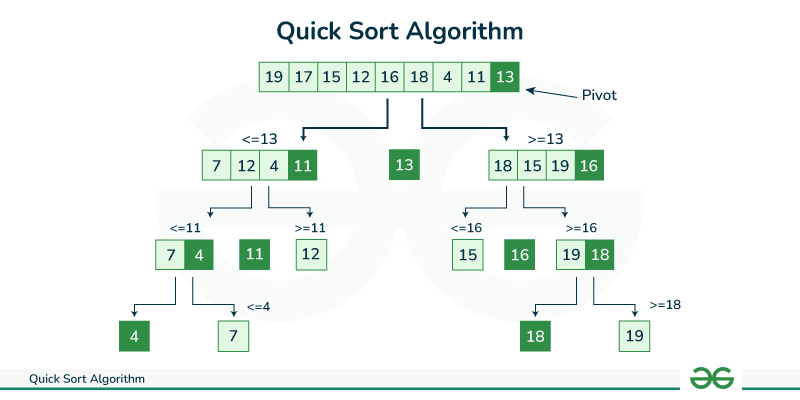
\includegraphics[keepaspectratio]{images/0_vAMz_7iAbCplF4Z7.png}}

}

\caption{Quick\_sort}

\end{figure}%

Particion y pivote

\begin{enumerate}
\def\labelenumi{\arabic{enumi}.}
\item
  \textbf{Pivote}: Es el elemento alrededor del cual se divide la
  matriz, por ende, se puede elgir cualquier elemtno como pivote, pero
  las estrategias mcomunes incluyen la selección del primer elemento, el
  último elemento o un elemento aleatorio.
\item
  \textbf{Partición}: SU objetivo es mover todos los elementos más
  pequeños que el pivote a su izquierda y todos los elementos más
  grandes a su derecha.
\end{enumerate}

\subsection[Implementación en Java \begin{center}

\end{center}
]{\texorpdfstring{Implementación en Java \begin{center}
\protect
\includegraphics[width=0.7\linewidth,height=\textheight,keepaspectratio]{images/java111.png}
\end{center}
}{Implementación en Java }}\label{implementaciuxf3n-en-java-2}

Implementaremos \texttt{quick\_sort} en Java. Esta implementación es una
versión simplificada que crea nuevos arrays en cada paso de la
partición, lo cual es más fácil de entender pero menos eficiente en
espacio que una implementación ``in-place'' con índices.

\begin{Shaded}
\begin{Highlighting}[]
\KeywordTok{public} \KeywordTok{class}\NormalTok{ QuickSort }\OperatorTok{\{}
    
    \KeywordTok{public} \DataTypeTok{static} \DataTypeTok{int}\OperatorTok{[]} \FunctionTok{quick\_sort}\OperatorTok{(}\DataTypeTok{int}\OperatorTok{[]}\NormalTok{ arr}\OperatorTok{)} \OperatorTok{\{}
        \DataTypeTok{int}\NormalTok{ n }\OperatorTok{=}\NormalTok{ arr}\OperatorTok{.}\FunctionTok{length}\OperatorTok{;}
        
\NormalTok{        \# Caso base}\OperatorTok{:}\NormalTok{ un array con }\DecValTok{0}\NormalTok{ o }\DecValTok{1}\NormalTok{ elemento ya está ordenado}
        \ControlFlowTok{if} \OperatorTok{(}\NormalTok{n }\OperatorTok{\textless{}=} \DecValTok{1}\OperatorTok{)} \OperatorTok{\{}
            \ControlFlowTok{return}\NormalTok{ arr}\OperatorTok{;}
        \OperatorTok{\}}
        
\NormalTok{        \# Elegir un pivote}\OperatorTok{.} \FunctionTok{Aqu}\NormalTok{í usamos el último elemento por simplicidad}\OperatorTok{.}
\NormalTok{        \# Otras estrategias incluyen elegir el primero}\OperatorTok{,}\NormalTok{ el del medio}\OperatorTok{,}\NormalTok{ o un pivote aleatorio}\OperatorTok{.}
        \FunctionTok{int}\NormalTok{ pivot\_index }\OperatorTok{=}\NormalTok{ n }\OperatorTok{{-}} \DecValTok{1}\OperatorTok{;}
        \DataTypeTok{int}\NormalTok{ pivot }\OperatorTok{=}\NormalTok{ arr}\OperatorTok{[}\NormalTok{pivot\_index}\OperatorTok{];}
        
\NormalTok{        \# Separar los elementos menores y mayores que el pivote}
\NormalTok{        \# Excluimos el pivote del array original antes de la partición}
        \DataTypeTok{int}\OperatorTok{[]}\NormalTok{ remaining\_elements }\OperatorTok{=} \KeywordTok{new} \DataTypeTok{int}\OperatorTok{[}\NormalTok{n }\OperatorTok{{-}} \DecValTok{1}\OperatorTok{];}
        \ControlFlowTok{for} \OperatorTok{(}\DataTypeTok{int}\NormalTok{ i }\OperatorTok{=} \DecValTok{0}\OperatorTok{,}\NormalTok{ j }\OperatorTok{=} \DecValTok{0}\OperatorTok{;}\NormalTok{ i }\OperatorTok{\textless{}}\NormalTok{ n}\OperatorTok{;}\NormalTok{ i}\OperatorTok{++)} \OperatorTok{\{}
            \ControlFlowTok{if} \OperatorTok{(}\NormalTok{i }\OperatorTok{!=}\NormalTok{ pivot\_index}\OperatorTok{)} \OperatorTok{\{}
\NormalTok{                remaining\_elements}\OperatorTok{[}\NormalTok{j}\OperatorTok{++]} \OperatorTok{=}\NormalTok{ arr}\OperatorTok{[}\NormalTok{i}\OperatorTok{];}
            \OperatorTok{\}}
        \OperatorTok{\}}
        
\NormalTok{        \# Utilizar un enfoque para la partición}
\NormalTok{        \# Esto crea nuevos arrays}\OperatorTok{,}\NormalTok{ lo que impacta la eficiencia espacial}
\NormalTok{        \# Contar elementos menores y mayores}
        \DataTypeTok{int}\NormalTok{ lessCount }\OperatorTok{=} \DecValTok{0}\OperatorTok{,}\NormalTok{ greaterCount }\OperatorTok{=} \DecValTok{0}\OperatorTok{;}
        \ControlFlowTok{for} \OperatorTok{(}\DataTypeTok{int}\NormalTok{ num }\OperatorTok{:}\NormalTok{ remaining\_elements}\OperatorTok{)} \OperatorTok{\{}
            \ControlFlowTok{if} \OperatorTok{(}\NormalTok{num }\OperatorTok{\textless{}}\NormalTok{ pivot}\OperatorTok{)} \OperatorTok{\{}
\NormalTok{                lessCount}\OperatorTok{++;}
            \OperatorTok{\}} \ControlFlowTok{else} \OperatorTok{\{}
\NormalTok{                greaterCount}\OperatorTok{++;}
            \OperatorTok{\}}
        \OperatorTok{\}}
        
\NormalTok{        \# Crear arrays para less y greater}
        \DataTypeTok{int}\OperatorTok{[]}\NormalTok{ less }\OperatorTok{=} \KeywordTok{new} \DataTypeTok{int}\OperatorTok{[}\NormalTok{lessCount}\OperatorTok{];}
        \DataTypeTok{int}\OperatorTok{[]}\NormalTok{ greater }\OperatorTok{=} \KeywordTok{new} \DataTypeTok{int}\OperatorTok{[}\NormalTok{greaterCount}\OperatorTok{];}
        
\NormalTok{        \# Llenar los arrays}
        \DataTypeTok{int}\NormalTok{ lessIdx }\OperatorTok{=} \DecValTok{0}\OperatorTok{,}\NormalTok{ greaterIdx }\OperatorTok{=} \DecValTok{0}\OperatorTok{;}
        \ControlFlowTok{for} \OperatorTok{(}\DataTypeTok{int}\NormalTok{ num }\OperatorTok{:}\NormalTok{ remaining\_elements}\OperatorTok{)} \OperatorTok{\{}
            \ControlFlowTok{if} \OperatorTok{(}\NormalTok{num }\OperatorTok{\textless{}}\NormalTok{ pivot}\OperatorTok{)} \OperatorTok{\{}
\NormalTok{                less}\OperatorTok{[}\NormalTok{lessIdx}\OperatorTok{++]} \OperatorTok{=}\NormalTok{ num}\OperatorTok{;}
            \OperatorTok{\}} \ControlFlowTok{else} \OperatorTok{\{}
\NormalTok{                greater}\OperatorTok{[}\NormalTok{greaterIdx}\OperatorTok{++]} \OperatorTok{=}\NormalTok{ num}\OperatorTok{;}\NormalTok{ \# }\OperatorTok{\textgreater{}=}\NormalTok{ para incluir iguales o mayores}
            \OperatorTok{\}}
        \OperatorTok{\}}
        
\NormalTok{        \# Ordenar recursivamente las sublistas y combinar}
        \DataTypeTok{int}\OperatorTok{[]}\NormalTok{ sortedLess }\OperatorTok{=} \FunctionTok{quick\_sort}\OperatorTok{(}\NormalTok{less}\OperatorTok{);}
        \DataTypeTok{int}\OperatorTok{[]}\NormalTok{ sortedGreater }\OperatorTok{=} \FunctionTok{quick\_sort}\OperatorTok{(}\NormalTok{greater}\OperatorTok{);}
        
\NormalTok{        \# Combinar}\OperatorTok{:}\NormalTok{ sortedLess }\OperatorTok{+}\NormalTok{ pivot }\OperatorTok{+}\NormalTok{ sortedGreater}
        \DataTypeTok{int}\OperatorTok{[]}\NormalTok{ result }\OperatorTok{=} \KeywordTok{new} \DataTypeTok{int}\OperatorTok{[}\NormalTok{sortedLess}\OperatorTok{.}\FunctionTok{length} \OperatorTok{+} \DecValTok{1} \OperatorTok{+}\NormalTok{ sortedGreater}\OperatorTok{.}\FunctionTok{length}\OperatorTok{];}
        \BuiltInTok{System}\OperatorTok{.}\FunctionTok{arraycopy}\OperatorTok{(}\NormalTok{sortedLess}\OperatorTok{,} \DecValTok{0}\OperatorTok{,}\NormalTok{ result}\OperatorTok{,} \DecValTok{0}\OperatorTok{,}\NormalTok{ sortedLess}\OperatorTok{.}\FunctionTok{length}\OperatorTok{);}
\NormalTok{        result}\OperatorTok{[}\NormalTok{sortedLess}\OperatorTok{.}\FunctionTok{length}\OperatorTok{]} \OperatorTok{=}\NormalTok{ pivot}\OperatorTok{;}
        \BuiltInTok{System}\OperatorTok{.}\FunctionTok{arraycopy}\OperatorTok{(}\NormalTok{sortedGreater}\OperatorTok{,} \DecValTok{0}\OperatorTok{,}\NormalTok{ result}\OperatorTok{,}\NormalTok{ sortedLess}\OperatorTok{.}\FunctionTok{length} \OperatorTok{+} \DecValTok{1}\OperatorTok{,} 
\NormalTok{        sortedGreater}\OperatorTok{.}\FunctionTok{length}\OperatorTok{);}
        
        \ControlFlowTok{return}\NormalTok{ result}\OperatorTok{;}
    \OperatorTok{\}}
\OperatorTok{\}}
\end{Highlighting}
\end{Shaded}

\subsection{Explicación del Código}\label{explicaciuxf3n-del-cuxf3digo}

\begin{enumerate}
\def\labelenumi{\arabic{enumi}.}
\tightlist
\item
  \textbf{\texttt{quickSort(int{[}{]}\ arr)}}: Nuestra función toma un
  array de enteros \texttt{arr}.
\item
  \textbf{\texttt{if\ (n\ \textless{}=\ 1)}}: El \textbf{caso base} de
  la recursión. Si el array tiene 0 o 1 elemento, se devuelve tal cual.
\item
  \textbf{\texttt{pivot\_index\ =\ n\ -\ 1} /
  \texttt{pivot\ =\ arr{[}pivot\_index{]}}}: Elegimos el último elemento
  como pivote. Esta es una elección simple, pero puede llevar al peor
  caso si el array ya está ordenado o casi ordenado.
\item
  \textbf{\texttt{remaining\_elements}}: Creamos un nuevo array que
  contiene todos los elementos excepto el pivote.
\item
  \textbf{\texttt{less\ y\ greater}}: Filtramos los elementos en dos
  arrays:

  \begin{itemize}
  \tightlist
  \item
    \textbf{less}: elementos menores que el pivote
  \item
    \textbf{greater}: elementos mayores o iguales que el pivote
  \end{itemize}
\item
  \textbf{\texttt{sortedLess\ =\ quickSort(less)\ y\ sortedGreater\ =\ quickSort(greater)}}:
  Llamadas recursivas para ordenar cada subarray.
\item
  \textbf{\texttt{return\ result}}: Esta es la fase de combinación.

  \begin{itemize}
  \tightlist
  \item
    Concatena \texttt{sorteddLess}, el \texttt{pivot} y
    \texttt{sortedGreater} en un nuevo array.
  \item
    \texttt{System.arraycopy()} se usa para copiar eficientemente los
    elementos.
  \end{itemize}
\end{enumerate}

\subsection{Complejidad del
Algoritmo}\label{complejidad-del-algoritmo-3}

\begin{itemize}
\tightlist
\item
  \textbf{Complejidad temporal}:

  \begin{itemize}
  \tightlist
  \item
    \textbf{Mejor caso}: (O(n log n)). Ocurre cuando el pivote divide el
    array en dos mitades aproximadamente iguales.
  \item
    \textbf{Caso promedio}: O(n log n). Con pivotes aleatorios o datos
    distribuidos uniformemente.
  \item
    \textbf{Peor caso}: O(n²): Cuando el pivote siempre es el elemento
    más pequeño o más grande.
  \end{itemize}
\item
  \textbf{Complejidad espacial}:

  \begin{itemize}
  \tightlist
  \item
    \textbf{O(n log n) en el peor caso}: Debido a que creamos nuevos
    arrays en cada nivel de recursión.
  \item
    Nuestra implementación en java, no es ``in-place'' por lo que
    utiliza más memoria que una versión optimizada con índices.
  \end{itemize}
\end{itemize}

\subsection{Ejemplo}\label{ejemplo-5}

Veamos \texttt{quick\_sort} en acción.

\begin{Shaded}
\begin{Highlighting}[]
\NormalTok{\# Ejemplo }\DecValTok{1}\OperatorTok{:}\NormalTok{ Un vector desordenado}
\DataTypeTok{int}\OperatorTok{[]}\NormalTok{ vector\_desordenado }\OperatorTok{=} \OperatorTok{\{}\DecValTok{10}\OperatorTok{,} \DecValTok{80}\OperatorTok{,} \DecValTok{30}\OperatorTok{,} \DecValTok{90}\OperatorTok{,} \DecValTok{40}\OperatorTok{,} \DecValTok{50}\OperatorTok{,} \DecValTok{70}\OperatorTok{\};}
\BuiltInTok{System}\OperatorTok{.}\FunctionTok{out}\OperatorTok{.}\FunctionTok{print}\OperatorTok{(}\StringTok{"Vector original: "} \OperatorTok{+} \BuiltInTok{Arrays}\OperatorTok{.}\FunctionTok{toString}\OperatorTok{(}\NormalTok{vector\_desordenado}\OperatorTok{));}
\DataTypeTok{int}\OperatorTok{[]}\NormalTok{ vector\_ordenado }\OperatorTok{=} \FunctionTok{quick\_sort}\OperatorTok{(}\NormalTok{vector\_desordenado}\OperatorTok{);}
\BuiltInTok{System}\OperatorTok{.}\FunctionTok{out}\OperatorTok{.}\FunctionTok{print}\OperatorTok{(}\StringTok{"Vector ordenado (Quicksort): "} \OperatorTok{+} \BuiltInTok{Arrays}\OperatorTok{.}\FunctionTok{toString}\OperatorTok{(}\NormalTok{vector\_ordenado}\OperatorTok{));}

\NormalTok{\# Ejemplo }\DecValTok{2}\OperatorTok{:}\NormalTok{ Un vector con números negativos}
\DataTypeTok{int}\OperatorTok{[]}\NormalTok{ vector\_negativos }\OperatorTok{=} \OperatorTok{\{{-}}\DecValTok{5}\OperatorTok{,} \DecValTok{3}\OperatorTok{,} \OperatorTok{{-}}\DecValTok{1}\OperatorTok{,} \DecValTok{8}\OperatorTok{,} \DecValTok{0}\OperatorTok{,} \OperatorTok{{-}}\DecValTok{10}\OperatorTok{\};}
\BuiltInTok{System}\OperatorTok{.}\FunctionTok{out}\OperatorTok{.}\FunctionTok{print}\OperatorTok{(}\StringTok{"Vector con negativos: "} \OperatorTok{+} \BuiltInTok{Arrays}\OperatorTok{.}\FunctionTok{toString}\OperatorTok{(}\NormalTok{vector\_negativos}\OperatorTok{));}
\DataTypeTok{int}\OperatorTok{[]}\NormalTok{ vector\_ordenado\_neg }\OperatorTok{=} \FunctionTok{quick\_sort}\OperatorTok{(}\NormalTok{vector\_negativos}\OperatorTok{);}
\BuiltInTok{System}\OperatorTok{.}\FunctionTok{out}\OperatorTok{.}\FunctionTok{print}\OperatorTok{(}\StringTok{"Vector ordenado (Quicksort): "} \OperatorTok{+} \BuiltInTok{Arrays}\OperatorTok{.}\FunctionTok{toString}\OperatorTok{(}\NormalTok{vector\_ordenado\_neg}\OperatorTok{));}
\end{Highlighting}
\end{Shaded}

\subsection[Implementación en Python \begin{center}

\end{center}
]{\texorpdfstring{Implementación en Python \begin{center}
\protect
\includegraphics[width=0.7\linewidth,height=\textheight,keepaspectratio]{images/Python.svg.png}
\end{center}
}{Implementación en Python }}\label{implementaciuxf3n-en-python-2}

Implementaremos \texttt{quick\_sort} en Java. Esta implementacion es una
versión simplificada que crea nueva listas en cada paso de la partición,
lo cual es más idiomático en Python pero menos eficiente en especio que
una implementación ``in-place'' con índices.

\begin{Shaded}
\begin{Highlighting}[]
\KeywordTok{def}\NormalTok{ quick\_sort(arr):}
\NormalTok{    n }\OperatorTok{=} \BuiltInTok{len}\NormalTok{(arr)}
    
    \CommentTok{\# Caso base: una lista con 0 o 1 elemento ya está ordenada}
    \ControlFlowTok{if}\NormalTok{ n }\OperatorTok{\textless{}=} \DecValTok{1}\NormalTok{:}
        \ControlFlowTok{return}\NormalTok{ arr}
    
    \CommentTok{\# Elegir un pivote. Aquí se usa el último elemento por simplicidad.}
    \CommentTok{\# Otras estrategias incluyen elegir el primero, el del medio, o un pivote aleatorio.}
\NormalTok{    pivot\_index }\OperatorTok{=}\NormalTok{ n }\OperatorTok{{-}} \DecValTok{1}
\NormalTok{    pivot }\OperatorTok{=}\NormalTok{ arr[pivot\_index]}
    
    \CommentTok{\# Separar los elementos menores y mayores que el pivote}
    \CommentTok{\# Excluimos el pivote de la lista original antes de la partición}
\NormalTok{    remaining\_elements }\OperatorTok{=}\NormalTok{ arr[:pivot\_index] }\OperatorTok{+}\NormalTok{ arr[pivot\_index }\OperatorTok{+} \DecValTok{1}\NormalTok{:]}
    
    \CommentTok{\# Utilizar un enfoque Python{-}idiomático para la partición}
    \CommentTok{\# Esto crea nuevas listas, lo que impacta la eficiencia espacial}
\NormalTok{    less }\OperatorTok{=}\NormalTok{ [x }\ControlFlowTok{for}\NormalTok{ x }\KeywordTok{in}\NormalTok{ remaining\_elements }\ControlFlowTok{if}\NormalTok{ x }\OperatorTok{\textless{}}\NormalTok{ pivot]}
\NormalTok{    greater }\OperatorTok{=}\NormalTok{ [x }\ControlFlowTok{for}\NormalTok{ x }\KeywordTok{in}\NormalTok{ remaining\_elements }\ControlFlowTok{if}\NormalTok{ x }\OperatorTok{\textgreater{}=}\NormalTok{ pivot]  }\CommentTok{\# \textgreater{}= para incluir iguales o mayores}
    
    \CommentTok{\# Ordenar recursivamente las sublistas y combinar}
    \ControlFlowTok{return}\NormalTok{ quick\_sort(less) }\OperatorTok{+}\NormalTok{ [pivot] }\OperatorTok{+}\NormalTok{ quick\_sort(greater)}
\end{Highlighting}
\end{Shaded}

\subsection{Explicación del
Código}\label{explicaciuxf3n-del-cuxf3digo-1}

\begin{enumerate}
\def\labelenumi{\arabic{enumi}.}
\tightlist
\item
  \textbf{\texttt{quickSort(int{[}{]}\ arr)}}: Nuestra función toma una
  lista \texttt{arr}.
\item
  \textbf{\texttt{if\ (n\ \textless{}=\ 1)}}: El \textbf{caso base} de
  la recursión. Si la lista tiene 0 o 1 elemento, se devuelve tal cual.
\item
  \textbf{\texttt{pivot\_index\ =\ n\ -\ 1} /
  \texttt{pivot\ =\ arr{[}pivot\_index{]}}}: Elegimos el último elemento
  como pivote. Esta es una elección simple, pero puede llevar al peor
  caso si la lista ya está ordenada o casi ordenada.
\item
  \textbf{\texttt{remaining\_elements\ =\ arr\ {[}:pivot\_index{]}\ +\ arr{[}pivot\_index\ +\ 1{]}}}:
  Creamos una nueva lista que contiene todos los elementos excepto el
  pivote.
\item
  \textbf{\texttt{less\ =\ {[}x\ for\ x\ in\ remaining\_elements\ if\ x\ \textgreater{}=\ pivot{]}}}:
  Filtra los elementos que son mayores o iguales que el pivote, por
  ende, es importante incluir los iguales para evitar bucles infinitos
  en casos con duplicados si solo se usara
  \textbf{\texttt{\textgreater{}}} y el pivote fuera único.
\item
  \textbf{\texttt{return\ quick\_sort(less)\ +\ {[}pivot{]}\ +\ quick\_sort(greater)}}:
  Esta es la fase de combinación

  \begin{itemize}
  \tightlist
  \item
    Llama recursivamente a \textbf{quick\_sort} en la sublista
    \textbf{\texttt{less}}
  \item
    EL \textbf{pivot} se coloca en medio, ya que está en su posición
    final
  \item
    Llama recursivamente a \textbf{\texttt{quick\_sort}} en la sublista
    \textbf{\texttt{greater}}
  \item
    EL operador \textbf{\texttt{+}} concatena estas tres listas en la
    lista final ordenada.
  \end{itemize}
\end{enumerate}

\subsection{Complejidad del
Algoritmo}\label{complejidad-del-algoritmo-4}

\begin{itemize}
\tightlist
\item
  \textbf{Complejidad temporal}:

  \begin{itemize}
  \tightlist
  \item
    \textbf{Mejor caso}: O(n log n). Ocurre cuando el pivote divide la
    lista en dos mitades aproximadamente iguales
  \item
    \textbf{Caso promedio}: O(n log n). Con pivotes aleatorios o datos
    distribuidos uniformemente.
  \item
    \textbf{Peor caso}: O(n²): Ocurre cuando el pivote siempre es el
    elemento más pequeño o más grande
  \end{itemize}
\item
  \textbf{Complejidad espacial}:

  \begin{itemize}
  \tightlist
  \item
    \textbf{O(n log n) en el peor caso}: Debido a que creamos nuevas
    listas en cada nivel de recursión.
  \item
    Esta implementación no es ``in-place'', por lo que utiliza más
    memoria que una versión optimizada con índices.
  \end{itemize}
\end{itemize}

\subsection{Ejemplo}\label{ejemplo-6}

Veamos \texttt{quick\_sort} en acción.

\begin{Shaded}
\begin{Highlighting}[]
\CommentTok{\# Ejemplo 1: Una lista desordenada}
\NormalTok{vector\_desordenado }\OperatorTok{=}\NormalTok{ [}\DecValTok{10}\NormalTok{, }\DecValTok{80}\NormalTok{, }\DecValTok{30}\NormalTok{, }\DecValTok{90}\NormalTok{, }\DecValTok{40}\NormalTok{, }\DecValTok{50}\NormalTok{, }\DecValTok{70}\NormalTok{]}
\BuiltInTok{print}\NormalTok{(}\SpecialStringTok{f"Vector original: }\SpecialCharTok{\{}\NormalTok{vector\_desordenado}\SpecialCharTok{\}}\SpecialStringTok{"}\NormalTok{)}
\NormalTok{vector\_ordenado }\OperatorTok{=}\NormalTok{ quick\_sort(vector\_desordenado)}
\BuiltInTok{print}\NormalTok{(}\SpecialStringTok{f"Vector ordenado (Quicksort): }\SpecialCharTok{\{}\NormalTok{vector\_ordenado}\SpecialCharTok{\}}\SpecialStringTok{"}\NormalTok{)}

\CommentTok{\# Ejemplo 2: Una lista con números negativos}
\NormalTok{vector\_negativos }\OperatorTok{=}\NormalTok{ [}\OperatorTok{{-}}\DecValTok{5}\NormalTok{, }\DecValTok{3}\NormalTok{, }\OperatorTok{{-}}\DecValTok{1}\NormalTok{, }\DecValTok{8}\NormalTok{, }\DecValTok{0}\NormalTok{, }\OperatorTok{{-}}\DecValTok{10}\NormalTok{]}
\BuiltInTok{print}\NormalTok{(}\SpecialStringTok{f"Vector con negativos: }\SpecialCharTok{\{}\NormalTok{vector\_negativos}\SpecialCharTok{\}}\SpecialStringTok{"}\NormalTok{)}
\NormalTok{vector\_ordenado\_neg }\OperatorTok{=}\NormalTok{ quick\_sort(vector\_negativos)}
\BuiltInTok{print}\NormalTok{(}\SpecialStringTok{f"Vector ordenado (Quicksort): }\SpecialCharTok{\{}\NormalTok{vector\_ordenado\_neg}\SpecialCharTok{\}}\SpecialStringTok{"}\NormalTok{)}

\CommentTok{\# Ejemplo 3: Una lista con elementos duplicados}
\NormalTok{vector\_duplicados }\OperatorTok{=}\NormalTok{ [}\DecValTok{5}\NormalTok{, }\DecValTok{2}\NormalTok{, }\DecValTok{8}\NormalTok{, }\DecValTok{2}\NormalTok{, }\DecValTok{5}\NormalTok{, }\DecValTok{1}\NormalTok{, }\DecValTok{8}\NormalTok{]}
\BuiltInTok{print}\NormalTok{(}\SpecialStringTok{f"Vector con duplicados: }\SpecialCharTok{\{}\NormalTok{vector\_duplicados}\SpecialCharTok{\}}\SpecialStringTok{"}\NormalTok{)}
\NormalTok{vector\_ordenado\_dup }\OperatorTok{=}\NormalTok{ quick\_sort(vector\_duplicados)}
\BuiltInTok{print}\NormalTok{(}\SpecialStringTok{f"Vector ordenado (Quicksort): }\SpecialCharTok{\{}\NormalTok{vector\_ordenado\_dup}\SpecialCharTok{\}}\SpecialStringTok{"}\NormalTok{)}
\end{Highlighting}
\end{Shaded}

\subsection[Implementación en JavaScript \begin{center}

\end{center}
]{\texorpdfstring{Implementación en JavaScript \begin{center}
\protect
\includegraphics[width=0.7\linewidth,height=\textheight,keepaspectratio]{images/js.png}
\end{center}
}{Implementación en JavaScript }}\label{implementaciuxf3n-en-javascript-2}

Implementaremos \texttt{quick\_sort} en JavaScript. Esta implementacion
es unaversión simplificada que crea nuevos arrays en cada paso de la
partición, lo cual es más idiomático en JavaScript pero menos eficiente
en especio que una implementación ``in-place'' con índices.

\begin{Shaded}
\begin{Highlighting}[]
\KeywordTok{function} \FunctionTok{quick\_sort}\NormalTok{(arr) \{}
    \KeywordTok{const}\NormalTok{ n }\OperatorTok{=}\NormalTok{ arr}\OperatorTok{.}\AttributeTok{length}\OperatorTok{;}
    
\NormalTok{    \# Caso }\DataTypeTok{base}\OperatorTok{:}\NormalTok{ un array con }\DecValTok{0}\NormalTok{ o }\DecValTok{1}\NormalTok{ elemento ya está ordenado}
    \ControlFlowTok{if}\NormalTok{ (n }\OperatorTok{\textless{}=} \DecValTok{1}\NormalTok{) \{}
        \ControlFlowTok{return}\NormalTok{ arr}\OperatorTok{;}
\NormalTok{    \}}
    
\NormalTok{    \# Elegir un pivote}\OperatorTok{.} \AttributeTok{Aquí}\NormalTok{ se usa el último elemento por simplicidad}\OperatorTok{.}
\NormalTok{    \# Otras estrategias incluyen elegir el primero}\OperatorTok{,}\NormalTok{ el del medio}\OperatorTok{,}\NormalTok{ o un pivote aleatorio}\OperatorTok{.}
    \KeywordTok{const}\NormalTok{ pivot\_index }\OperatorTok{=}\NormalTok{ n }\OperatorTok{{-}} \DecValTok{1}\OperatorTok{;}
    \KeywordTok{const}\NormalTok{ pivot }\OperatorTok{=}\NormalTok{ arr[pivot\_index]}\OperatorTok{;}
    
\NormalTok{    \# Separar los elementos menores y mayores que el pivote}
\NormalTok{    \# Excluimos el pivote del array original antes de la partición}
    \KeywordTok{const}\NormalTok{ remaining\_elements }\OperatorTok{=}\NormalTok{ arr}\OperatorTok{.}\FunctionTok{slice}\NormalTok{(}\DecValTok{0}\OperatorTok{,}\NormalTok{ pivot\_index)}\OperatorTok{.}\FunctionTok{concat}\NormalTok{(arr}\OperatorTok{.}\FunctionTok{slice}\NormalTok{(pivot\_index }\OperatorTok{+} \DecValTok{1}\NormalTok{))}\OperatorTok{;}
    
\NormalTok{    \# Utilizar un enfoque JavaScript}\OperatorTok{{-}}\NormalTok{idiomático para la partición}
\NormalTok{    \# Esto crea nuevos arrays}\OperatorTok{,}\NormalTok{ lo que impacta la eficiencia espacial}
    \KeywordTok{const}\NormalTok{ less }\OperatorTok{=}\NormalTok{ remaining\_elements}\OperatorTok{.}\FunctionTok{filter}\NormalTok{(x }\KeywordTok{=\textgreater{}}\NormalTok{ x }\OperatorTok{\textless{}}\NormalTok{ pivot)}\OperatorTok{;}
    \KeywordTok{const}\NormalTok{ greater }\OperatorTok{=}\NormalTok{ remaining\_elements}\OperatorTok{.}\FunctionTok{filter}\NormalTok{(x }\KeywordTok{=\textgreater{}}\NormalTok{ x }\OperatorTok{\textgreater{}=}\NormalTok{ pivot)}\OperatorTok{;}\NormalTok{ \# }\OperatorTok{\textgreater{}=}\NormalTok{ para incluir iguales o mayores}
    
\NormalTok{    \# Ordenar recursivamente las sublistas y combinar}
    \ControlFlowTok{return}\NormalTok{ [}\OperatorTok{...}\FunctionTok{quick\_sort}\NormalTok{(less)}\OperatorTok{,}\NormalTok{ pivot}\OperatorTok{,} \OperatorTok{...}\FunctionTok{quick\_sort}\NormalTok{(greater)]}\OperatorTok{;}
\NormalTok{\}}
\end{Highlighting}
\end{Shaded}

\subsection{Explicación del
Código}\label{explicaciuxf3n-del-cuxf3digo-2}

\begin{enumerate}
\def\labelenumi{\arabic{enumi}.}
\tightlist
\item
  \textbf{\texttt{quickSort(int{[}{]}\ arr)}}: Nuestra función toma una
  array \texttt{arr}.
\item
  \textbf{\texttt{if\ (n\ \textless{}=\ 1)}}: El \textbf{caso base} de
  la recursión. Si el array tiene 0 o 1 elemento, se devuelve tal cual.
\item
  \textbf{\texttt{pivot\_index\ =\ n\ -\ 1} /
  \texttt{pivot\ =\ arr{[}pivot\_index{]}}}: Elegimos el último elemento
  como pivote. Esta es una elección simple, pero puede llevar al peor
  caso si el array ya está ordenado o casi ordenado.
\item
  \textbf{\texttt{remaining\_elements}}: Creamos un array que contiene
  todos los elementos excepto el pivote usando \textbf{\texttt{slice()}}
  y \textbf{\texttt{concat()}} .
\item
  \textbf{\texttt{less\ =\ remaining\_elements.filter\ (x\ =\textgreater{}\ x\ \textless{}\ pivot)}}:
  Usamoe el método \textbf{\texttt{filter()}} para obtener los elementos
  \textbf{`remaining\_elements} que son menores que el pivote.
\item
  \textbf{\texttt{greater\ =\ remaining\_elements.filter(x\ =\textgreater{}\ x\ \textgreater{}=\ pivot)}}:
  Filtra los elementos que son mayores o iguales que el pivote
\item
  \textbf{\texttt{return\ {[}...quick\_sort(less),\ pivot,\ ...quick\_sort(greater){]}}}:
  Esta es la fase de combinacion

  \begin{itemize}
  \tightlist
  \item
    Llama recursivamente a \textbf{quick\_sort} en la sublista
    \textbf{\texttt{less}}
  \item
    EL \textbf{pivot} se coloca en medio, ya que está en su posición
    final
  \item
    Llama recursivamente a \textbf{\texttt{quick\_sort}} en la sublista
    \textbf{\texttt{greater}}
  \item
    EL operador spread \textbf{\texttt{...}} concatena estos tres
    resultados en el array final ordenado.
  \end{itemize}
\end{enumerate}

\subsection{Complejidad del
Algoritmo}\label{complejidad-del-algoritmo-5}

\begin{itemize}
\tightlist
\item
  \textbf{Complejidad temporal}:

  \begin{itemize}
  \tightlist
  \item
    \textbf{Mejor caso}: (O(n log n)). Ocurre cuando el pivote divide el
    array en dos mitades aproximadamente iguales
  \item
    \textbf{Caso promedio}: O(n log n). Con pivotes aleatorios o datos
    distribuidos uniformemente.
  \item
    \textbf{Peor caso}: O(n²): Ocurre cuando el pivote siempre es el
    elemento más pequeño o más grande
  \end{itemize}
\item
  \textbf{Complejidad espaciall}:

  \begin{itemize}
  \tightlist
  \item
    \textbf{O(n log n) en el peor caso}: Debido a que creamos nuevas
    listas en cada nivel de recursión.
  \item
    Esta implementación no es ``in-place'', por lo que utiliza más
    memoria que una versión optimizada con índices.
  \end{itemize}
\end{itemize}

\subsection{Ejemplo}\label{ejemplo-7}

Veamos \texttt{quick\_sort} en acción.

\begin{Shaded}
\begin{Highlighting}[]
\NormalTok{\# Ejemplo }\DecValTok{1}\OperatorTok{:}\NormalTok{ Una lista desordenada}
\KeywordTok{const}\NormalTok{ vector\_desordenado }\OperatorTok{=}\NormalTok{ [}\DecValTok{10}\OperatorTok{,} \DecValTok{80}\OperatorTok{,} \DecValTok{30}\OperatorTok{,} \DecValTok{90}\OperatorTok{,} \DecValTok{40}\OperatorTok{,} \DecValTok{50}\OperatorTok{,} \DecValTok{70}\NormalTok{]}\OperatorTok{;}
\BuiltInTok{console}\OperatorTok{.}\FunctionTok{log}\NormalTok{(}\VerbatimStringTok{\textasciigrave{}Vector original: }\SpecialCharTok{$\{}\NormalTok{vector\_desordenado}\SpecialCharTok{\}}\VerbatimStringTok{\textasciigrave{}}\NormalTok{)}\OperatorTok{;}
\KeywordTok{const}\NormalTok{ vector\_ordenado }\OperatorTok{=} \FunctionTok{quick\_sort}\NormalTok{(vector\_desordenado)}\OperatorTok{;}
\BuiltInTok{console}\OperatorTok{.}\FunctionTok{log}\NormalTok{(}\VerbatimStringTok{\textasciigrave{}Vector ordenado (Quicksort): }\SpecialCharTok{$\{}\NormalTok{vector\_ordenado}\SpecialCharTok{\}}\VerbatimStringTok{\textasciigrave{}}\NormalTok{)}\OperatorTok{;}

\NormalTok{\# Ejemplo }\DecValTok{2}\OperatorTok{:}\NormalTok{ Un array con números negativos}
\KeywordTok{const}\NormalTok{ vector\_negativos }\OperatorTok{=}\NormalTok{ [}\OperatorTok{{-}}\DecValTok{5}\OperatorTok{,} \DecValTok{3}\OperatorTok{,} \OperatorTok{{-}}\DecValTok{1}\OperatorTok{,} \DecValTok{8}\OperatorTok{,} \DecValTok{0}\OperatorTok{,} \OperatorTok{{-}}\DecValTok{10}\NormalTok{]}\OperatorTok{;}
\BuiltInTok{console}\OperatorTok{.}\FunctionTok{log}\NormalTok{(}\VerbatimStringTok{\textasciigrave{}Vector con negativos: }\SpecialCharTok{$\{}\NormalTok{vector\_negativos}\SpecialCharTok{\}}\VerbatimStringTok{\textasciigrave{}}\NormalTok{)}\OperatorTok{;}
\KeywordTok{const}\NormalTok{ vector\_ordenado\_neg }\OperatorTok{=} \FunctionTok{quick\_sort}\NormalTok{(vector\_negativos)}\OperatorTok{;}
\BuiltInTok{console}\OperatorTok{.}\FunctionTok{log}\NormalTok{(}\VerbatimStringTok{\textasciigrave{}Vector ordenado (Quicksort): }\SpecialCharTok{$\{}\NormalTok{vector\_ordenado\_neg}\SpecialCharTok{\}}\VerbatimStringTok{\textasciigrave{}}\NormalTok{)}\OperatorTok{;}

\NormalTok{\# Ejemplo }\DecValTok{3}\OperatorTok{:}\NormalTok{ Un array con elementos duplicados}
\KeywordTok{const}\NormalTok{ vector\_duplicados }\OperatorTok{=}\NormalTok{ [}\DecValTok{5}\OperatorTok{,} \DecValTok{2}\OperatorTok{,} \DecValTok{8}\OperatorTok{,} \DecValTok{2}\OperatorTok{,} \DecValTok{5}\OperatorTok{,} \DecValTok{1}\OperatorTok{,} \DecValTok{8}\NormalTok{]}\OperatorTok{;}
\BuiltInTok{console}\OperatorTok{.}\FunctionTok{log}\NormalTok{(}\VerbatimStringTok{\textasciigrave{}Vector con duplicados: }\SpecialCharTok{$\{}\NormalTok{vector\_duplicados}\SpecialCharTok{\}}\VerbatimStringTok{\textasciigrave{}}\NormalTok{)}\OperatorTok{;}
\KeywordTok{const}\NormalTok{ vector\_ordenado\_dup }\OperatorTok{=} \FunctionTok{quick\_sort}\NormalTok{(vector\_duplicados)}\OperatorTok{;}
\BuiltInTok{console}\OperatorTok{.}\FunctionTok{log}\NormalTok{(}\VerbatimStringTok{\textasciigrave{}Vector ordenado (Quicksort): }\SpecialCharTok{$\{}\NormalTok{vector\_ordenado\_dup}\SpecialCharTok{\}}\VerbatimStringTok{\textasciigrave{}}\NormalTok{)}\OperatorTok{;}
\end{Highlighting}
\end{Shaded}

\section{Conclusión}\label{conclusiuxf3n-1}

Se ha recorrido cuatro algoritmos de ordenación fundamentales, cada uno
con su enfoque único y características de rendimiento que definen su
utilidad y eficiencia en el desarrollo de software moderno.

\begin{tcolorbox}[enhanced jigsaw, arc=.35mm, bottomrule=.15mm, breakable, colback=white, colframe=quarto-callout-color-frame, left=2mm, leftrule=.75mm, opacityback=0, rightrule=.15mm, toprule=.15mm]

\begin{itemize}
\item
  \textbf{Bubble Sort} e \textbf{Insertion Sort} Son algoritmos
  intuitivos y eficientes lo cual los hacen ideal para comprender la
  lógica de control de flujos, asi mismo, son adecuados para colecciones
  pequeñas o datos que ya estan casi ordenados ya que requieren un
  número minimo de intercambios.

  Sin embargo, su complejidad 0(n²) provoca que el tiempo de ejecución
  se dispare ante volúmenes de datos medianos o grandes por lo que su
  uso es nulo frente a alternativas más escalabes.
\item
  \textbf{Mergesort} y \textbf{Quicksort} Estos algoritmos representan
  la eficiencia del paradigma ``divide y vencerás'', la cual consiste en
  fragmentar el problema original en partes mas pequeñas logrando
  generalmente un rendimiento de \textbf{O(n log n)}.

  \begin{itemize}
  \item
    \textbf{Mergesort} Es un algoritmo esable con una propiedad crítica
    cuando necesitamos que los elementos claves iguales mantengan su
    orden original.
  \item
    \textbf{Quicksort} Este es un algoritmo reconocido por ser el más
    veloz en la práctica debido a su baja carga administrativa y el
    aprovechamiento de la caché del procesador.
  \end{itemize}

  Al ser un algoritmo ``in-place'' es muy eficiente en el uso de memoria
  RAM donde depende de la elección del pivote, por lo que si escogemos
  mal la elección de datos ya ordenados puede degradar su rendimiento a
  \textbf{O(N²)}.
\end{itemize}

\end{tcolorbox}

No obstante, para la demostración de todos estos algoritmos de
ordenación usamos 3 lenguajes de programación, en este caso fue java,
pyhton y javascript. Aunque la sintaxis variaba un poco el
comportamiento era el mismo, cada uno se centraba en estructuras
estándar asegurando de no se altere el orden previo de elementos
iguales, demostrando que al implementar estos algoritmos en distintos
lenguajes no dependen simplemente de la herramienta, sino del dominio de
la complejidad algorítmica y la gestión de los recursos del sistema.

\section{Reto}\label{reto}

Imagina que tienes una caja llena de azulejos con letras (mayúsculas y
minúsculas) totalmente desordenadas. Tu objetivo es crear un programa
que saque todas las letras de la caja y las organice en una fila
perfectamente ordenada de la A a la Z. Escribe una función que reciba
una cadena de texto (la caja desordenada) y devuelva una nueva cadena
con las letras en orden alfabético.

\subsection{Restricciones}\label{restricciones}

\begin{enumerate}
\def\labelenumi{\arabic{enumi}.}
\setcounter{enumi}{1}
\tightlist
\item
  \textbf{Sin Librerías Externas:} Intenta programar la lógica de
  ordenamiento tú mismo en lugar de usar funciones automáticas del
  lenguaje (como .sort() o sorted()), para demostrar que entiendes cómo
  se mueven los datos
\item
  \textbf{Resultado Limpio:}: El resultado final debe ser una sola
  cadena de texto con todas las letras juntas y en orden.
\end{enumerate}

\subsection{Ejemplo}\label{ejemplo-8}

\begin{itemize}
\tightlist
\item
  \textbf{Entrada:} ``algoritmo''.
\item
  \textbf{Salida:} ``agilmort''.
\end{itemize}

Ahora la palabra ``algoritmo'' se encuentra ordenada en orden
alfabetico.

\bookmarksetup{startatroot}

\chapter{Algoritmos de Búsqueda}\label{algoritmos-de-buxfasqueda}

¡Hola a todos y bienvenidos a este capítulo sobre algoritmos de búsqueda
en R! Como analistas de datos, científicos de datos o simplemente
entusiastas de la programación, constantemente nos enfrentamos a la
tarea de encontrar elementos específicos dentro de colecciones de datos.
Ya sea que estemos buscando una transacción particular en un enorme
conjunto de datos financieros, un usuario específico en una base de
datos de millones de registros, o un valor dentro de un vector en R, la
eficiencia con la que realizamos estas búsquedas puede tener un impacto
significativo en el rendimiento de nuestras aplicaciones y en nuestro
tiempo de espera.

En este capítulo, exploraremos dos de los algoritmos de búsqueda más
fundamentales y ampliamente utilizados: la Búsqueda Secuencial (también
conocida como Búsqueda Lineal) y la Búsqueda Binaria. Entenderemos cómo
funcionan, cuándo usar cada uno y cómo implementarlos eficientemente en
R. ¡Prepárense para optimizar sus búsquedas!

\section{Búsqueda Secuencial (Linear
Search)}\label{buxfasqueda-secuencial-linear-search}

La búsqueda secuencial es el algoritmo de búsqueda más directo e
intuitivo. Imaginen que están buscando un libro específico en una
estantería desorganizada. Lo más lógico sería empezar por el primer
libro, revisarlo, luego pasar al segundo, y así sucesivamente, hasta que
encuentren el libro que buscan o hasta que se queden sin libros. Eso es
precisamente lo que hace la búsqueda secuencial.

Este algoritmo examina cada elemento de la colección uno por uno, en el
orden en que aparecen, hasta que encuentra el elemento deseado o hasta
que ha revisado todos los elementos sin éxito.

\subsection{¿Cómo funciona?}\label{cuxf3mo-funciona}

\begin{enumerate}
\def\labelenumi{\arabic{enumi}.}
\tightlist
\item
  Se inicia en el primer elemento de la colección.
\item
  Se compara el elemento actual con el valor objetivo que estamos
  buscando.
\item
  Si coinciden, la búsqueda termina y se devuelve la posición (índice)
  del elemento.
\item
  Si no coinciden, se avanza al siguiente elemento.
\item
  Este proceso se repite hasta que se encuentra el elemento o se alcanza
  el final de la colección.
\end{enumerate}

\subsection{Implementación en R}\label{implementaciuxf3n-en-r}

Vamos a implementar una función \texttt{busqueda\_secuencial} en R. Esta
función tomará un vector (\texttt{datos}) y un valor objetivo
(\texttt{objetivo}) como entrada.

\begin{Shaded}
\begin{Highlighting}[]
\CommentTok{\#\textquotesingle{} Función para realizar una búsqueda secuencial en un vector}
\CommentTok{\#\textquotesingle{}}
\CommentTok{\#\textquotesingle{} @param datos Un vector numérico o de caracteres donde buscar.}
\CommentTok{\#\textquotesingle{} @param objetivo El valor que se desea encontrar.}
\CommentTok{\#\textquotesingle{} @return El índice (posición) del objetivo si se encuentra, de lo contrario, NULL.}
\CommentTok{\#\textquotesingle{}}
\CommentTok{\#\textquotesingle{} @examples}
\CommentTok{\#\textquotesingle{} mi\_vector \textless{}{-} c(10, 5, 20, 15, 30, 25)}
\CommentTok{\#\textquotesingle{} busqueda\_secuencial(mi\_vector, 15) \# Debería devolver 4}
\CommentTok{\#\textquotesingle{} busqueda\_secuencial(mi\_vector, 99) \# Debería devolver NULL}
\NormalTok{busqueda\_secuencial }\OtherTok{\textless{}{-}} \ControlFlowTok{function}\NormalTok{(datos, objetivo) \{}
  \CommentTok{\# Recorremos el vector desde el primer elemento hasta el último}
  \ControlFlowTok{for}\NormalTok{ (i }\ControlFlowTok{in} \FunctionTok{seq\_along}\NormalTok{(datos)) \{}
    \CommentTok{\# Comparamos el elemento actual con el objetivo}
    \ControlFlowTok{if}\NormalTok{ (datos[i] }\SpecialCharTok{==}\NormalTok{ objetivo) \{}
      \CommentTok{\# Si coinciden, devolvemos su índice (posición)}
      \FunctionTok{message}\NormalTok{(}\FunctionTok{paste}\NormalTok{(}\StringTok{"Objetivo"}\NormalTok{, objetivo, }\StringTok{"encontrado en el índice"}\NormalTok{, i))}
      \FunctionTok{return}\NormalTok{(i)}
\NormalTok{    \}}
\NormalTok{  \}}
  \CommentTok{\# Si el bucle termina y no hemos encontrado el objetivo, devolvemos NULL}
  \FunctionTok{message}\NormalTok{(}\FunctionTok{paste}\NormalTok{(}\StringTok{"Objetivo"}\NormalTok{, objetivo, }\StringTok{"no encontrado en el vector."}\NormalTok{))}
  \FunctionTok{return}\NormalTok{(}\ConstantTok{NULL}\NormalTok{)}
\NormalTok{\}}
\end{Highlighting}
\end{Shaded}

\subsection{Ejemplos de Uso}\label{ejemplos-de-uso}

Veamos nuestra función en acción con algunos ejemplos.

\begin{Shaded}
\begin{Highlighting}[]
\CommentTok{\# Ejemplo 1: El objetivo está presente}
\NormalTok{numeros }\OtherTok{\textless{}{-}} \FunctionTok{c}\NormalTok{(}\DecValTok{4}\NormalTok{, }\DecValTok{2}\NormalTok{, }\DecValTok{7}\NormalTok{, }\DecValTok{1}\NormalTok{, }\DecValTok{9}\NormalTok{, }\DecValTok{5}\NormalTok{, }\DecValTok{8}\NormalTok{, }\DecValTok{3}\NormalTok{, }\DecValTok{6}\NormalTok{)}
\FunctionTok{busqueda\_secuencial}\NormalTok{(numeros, }\DecValTok{9}\NormalTok{)}
\end{Highlighting}
\end{Shaded}

\begin{verbatim}
Objetivo 9 encontrado en el índice 5
\end{verbatim}

\begin{verbatim}
[1] 5
\end{verbatim}

\begin{Shaded}
\begin{Highlighting}[]
\CommentTok{\# Ejemplo 2: El objetivo no está presente}
\FunctionTok{busqueda\_secuencial}\NormalTok{(numeros, }\DecValTok{10}\NormalTok{)}
\end{Highlighting}
\end{Shaded}

\begin{verbatim}
Objetivo 10 no encontrado en el vector.
\end{verbatim}

\begin{verbatim}
NULL
\end{verbatim}

\begin{Shaded}
\begin{Highlighting}[]
\CommentTok{\# Ejemplo 3: Con datos de texto}
\NormalTok{frutas }\OtherTok{\textless{}{-}} \FunctionTok{c}\NormalTok{(}\StringTok{"manzana"}\NormalTok{, }\StringTok{"platano"}\NormalTok{, }\StringTok{"cereza"}\NormalTok{, }\StringTok{"dátil"}\NormalTok{, }\StringTok{"elderberry"}\NormalTok{)}
\FunctionTok{busqueda\_secuencial}\NormalTok{(frutas, }\StringTok{"cereza"}\NormalTok{)}
\end{Highlighting}
\end{Shaded}

\begin{verbatim}
Objetivo cereza encontrado en el índice 3
\end{verbatim}

\begin{verbatim}
[1] 3
\end{verbatim}

\begin{Shaded}
\begin{Highlighting}[]
\FunctionTok{busqueda\_secuencial}\NormalTok{(frutas, }\StringTok{"kiwi"}\NormalTok{)}
\end{Highlighting}
\end{Shaded}

\begin{verbatim}
Objetivo kiwi no encontrado en el vector.
\end{verbatim}

\begin{verbatim}
NULL
\end{verbatim}

\begin{Shaded}
\begin{Highlighting}[]
\CommentTok{\# Ejemplo 4: El objetivo es el primer elemento}
\FunctionTok{busqueda\_secuencial}\NormalTok{(numeros, }\DecValTok{4}\NormalTok{)}
\end{Highlighting}
\end{Shaded}

\begin{verbatim}
Objetivo 4 encontrado en el índice 1
\end{verbatim}

\begin{verbatim}
[1] 1
\end{verbatim}

\begin{Shaded}
\begin{Highlighting}[]
\CommentTok{\# Ejemplo 5: El objetivo es el último elemento}
\FunctionTok{busqueda\_secuencial}\NormalTok{(numeros, }\DecValTok{6}\NormalTok{)}
\end{Highlighting}
\end{Shaded}

\begin{verbatim}
Objetivo 6 encontrado en el índice 9
\end{verbatim}

\begin{verbatim}
[1] 9
\end{verbatim}

\subsection{Eficiencia y Casos de Uso}\label{eficiencia-y-casos-de-uso}

La principal ventaja de la búsqueda secuencial es su simplicidad y que
no requiere que los datos estén ordenados. Sin embargo, su principal
desventaja es su eficiencia.

\begin{itemize}
\tightlist
\item
  \textbf{Complejidad Temporal (Worst Case):} O(n). En el peor de los
  casos (cuando el elemento no está presente o está al final), el
  algoritmo debe revisar todos los \texttt{n} elementos.
\item
  \textbf{Complejidad Temporal (Best Case):} O(1). En el mejor de los
  casos (cuando el elemento es el primero), solo necesita una
  comparación.
\item
  \textbf{Complejidad Temporal (Average Case):} O(n). En promedio,
  revisará \texttt{n/2} elementos.
\end{itemize}

La búsqueda secuencial es apropiada para: * Conjuntos de datos pequeños.
* Datos que no están ordenados y ordenar los datos sería más costoso que
realizar la búsqueda secuencial. * Cuando solo se necesitan realizar
unas pocas búsquedas.

Para conjuntos de datos grandes, la búsqueda secuencial puede ser muy
lenta. Es aquí donde la búsqueda binaria brilla.

\section{Búsqueda Binaria (Binary
Search)}\label{buxfasqueda-binaria-binary-search}

A diferencia de la búsqueda secuencial, la búsqueda binaria es un
algoritmo mucho más eficiente, pero tiene un requisito fundamental:
\textbf{los datos deben estar ordenados}.

Piensen en cómo buscan una palabra en un diccionario. No empiezan por la
primera palabra y revisan una por una. Abren el diccionario por la
mitad, miran si la palabra está antes o después, y luego descartan la
mitad del diccionario que no les sirve. Repiten este proceso en la mitad
restante hasta encontrar la palabra. La búsqueda binaria opera bajo el
mismo principio de ``divide y vencerás''.

\subsection{¿Cómo funciona?}\label{cuxf3mo-funciona-1}

\begin{enumerate}
\def\labelenumi{\arabic{enumi}.}
\tightlist
\item
  Asegurarse de que el vector esté \textbf{ordenado}. Si no lo está,
  primero deben ordenarlo.
\item
  Se define un rango de búsqueda dentro del vector, inicialmente todo el
  vector. Este rango está delimitado por un índice \texttt{inicio} y un
  índice \texttt{fin}.
\item
  Se calcula el índice del elemento central del rango:
  \texttt{medio\ =\ (inicio\ +\ fin)\ /\ 2}.
\item
  Se compara el elemento en la posición \texttt{medio} con el valor
  objetivo:

  \begin{itemize}
  \tightlist
  \item
    Si coinciden, el elemento ha sido encontrado y se devuelve
    \texttt{medio}.
  \item
    Si el elemento en \texttt{medio} es \textbf{menor} que el objetivo,
    significa que el objetivo (si existe) debe estar en la mitad
    \textbf{derecha} del rango. Se ajusta \texttt{inicio} a
    \texttt{medio\ +\ 1}.
  \item
    Si el elemento en \texttt{medio} es \textbf{mayor} que el objetivo,
    significa que el objetivo (si existe) debe estar en la mitad
    \textbf{izquierda} del rango. Se ajusta \texttt{fin} a
    \texttt{medio\ -\ 1}.
  \end{itemize}
\item
  Los pasos 2 a 4 se repiten hasta que el objetivo se encuentra o hasta
  que el rango de búsqueda se reduce a cero (lo que significa que el
  objetivo no está presente).
\end{enumerate}

\subsection{Implementación en R}\label{implementaciuxf3n-en-r-1}

Implementaremos una versión iterativa de la búsqueda binaria.

\begin{Shaded}
\begin{Highlighting}[]
\CommentTok{\#\textquotesingle{} Función para realizar una búsqueda binaria en un vector ordenado}
\CommentTok{\#\textquotesingle{}}
\CommentTok{\#\textquotesingle{} @param datos Un vector numérico o de caracteres ORDENADO donde buscar.}
\CommentTok{\#\textquotesingle{} @param objetivo El valor que se desea encontrar.}
\CommentTok{\#\textquotesingle{} @return El índice (posición) del objetivo si se encuentra, de lo contrario, NULL.}
\CommentTok{\#\textquotesingle{}}
\CommentTok{\#\textquotesingle{} @examples}
\CommentTok{\#\textquotesingle{} vector\_ordenado \textless{}{-} c(5, 10, 15, 20, 25, 30)}
\CommentTok{\#\textquotesingle{} busqueda\_binaria(vector\_ordenado, 20) \# Debería devolver 4}
\CommentTok{\#\textquotesingle{} busqueda\_binaria(vector\_ordenado, 12) \# Debería devolver NULL}
\NormalTok{busqueda\_binaria }\OtherTok{\textless{}{-}} \ControlFlowTok{function}\NormalTok{(datos, objetivo) \{}
  \CommentTok{\# Verificar que el vector no esté vacío}
  \ControlFlowTok{if}\NormalTok{ (}\FunctionTok{length}\NormalTok{(datos) }\SpecialCharTok{==} \DecValTok{0}\NormalTok{) \{}
    \FunctionTok{message}\NormalTok{(}\StringTok{"El vector está vacío."}\NormalTok{)}
    \FunctionTok{return}\NormalTok{(}\ConstantTok{NULL}\NormalTok{)}
\NormalTok{  \}}

  \CommentTok{\# Se asume que el vector \textquotesingle{}datos\textquotesingle{} ya está ordenado.}
  \CommentTok{\# Si no estuviera ordenado, necesitaríamos una línea como:}
  \CommentTok{\# datos \textless{}{-} sort(datos)}
  \CommentTok{\# Pero esto añade una complejidad O(n log n) y no es parte del algoritmo de búsqueda binaria en sí.}

\NormalTok{  inicio }\OtherTok{\textless{}{-}} \DecValTok{1}
\NormalTok{  fin }\OtherTok{\textless{}{-}} \FunctionTok{length}\NormalTok{(datos)}

  \ControlFlowTok{while}\NormalTok{ (inicio }\SpecialCharTok{\textless{}=}\NormalTok{ fin) \{}
    \CommentTok{\# Calcular el punto medio. Usamos floor para asegurar un índice entero.}
\NormalTok{    medio }\OtherTok{\textless{}{-}} \FunctionTok{floor}\NormalTok{((inicio }\SpecialCharTok{+}\NormalTok{ fin) }\SpecialCharTok{/} \DecValTok{2}\NormalTok{)}

    \CommentTok{\# Comparamos el elemento en el medio con el objetivo}
    \ControlFlowTok{if}\NormalTok{ (datos[medio] }\SpecialCharTok{==}\NormalTok{ objetivo) \{}
      \FunctionTok{message}\NormalTok{(}\FunctionTok{paste}\NormalTok{(}\StringTok{"Objetivo"}\NormalTok{, objetivo, }\StringTok{"encontrado en el índice"}\NormalTok{, medio))}
      \FunctionTok{return}\NormalTok{(medio) }\CommentTok{\# ¡Encontrado!}
\NormalTok{    \} }\ControlFlowTok{else} \ControlFlowTok{if}\NormalTok{ (datos[medio] }\SpecialCharTok{\textless{}}\NormalTok{ objetivo) \{}
      \CommentTok{\# El objetivo está en la mitad derecha}
\NormalTok{      inicio }\OtherTok{\textless{}{-}}\NormalTok{ medio }\SpecialCharTok{+} \DecValTok{1}
\NormalTok{    \} }\ControlFlowTok{else}\NormalTok{ \{}
      \CommentTok{\# El objetivo está en la mitad izquierda}
\NormalTok{      fin }\OtherTok{\textless{}{-}}\NormalTok{ medio }\SpecialCharTok{{-}} \DecValTok{1}
\NormalTok{    \}}
\NormalTok{  \}}

  \CommentTok{\# Si el bucle termina, el objetivo no fue encontrado}
  \FunctionTok{message}\NormalTok{(}\FunctionTok{paste}\NormalTok{(}\StringTok{"Objetivo"}\NormalTok{, objetivo, }\StringTok{"no encontrado en el vector."}\NormalTok{))}
  \FunctionTok{return}\NormalTok{(}\ConstantTok{NULL}\NormalTok{)}
\NormalTok{\}}
\end{Highlighting}
\end{Shaded}

\subsection{Ejemplos de Uso}\label{ejemplos-de-uso-1}

Recuerden, el vector DEBE estar ordenado para que la búsqueda binaria
funcione correctamente.

\begin{Shaded}
\begin{Highlighting}[]
\CommentTok{\# Creamos un vector ordenado}
\NormalTok{numeros\_ordenados }\OtherTok{\textless{}{-}} \FunctionTok{c}\NormalTok{(}\DecValTok{1}\NormalTok{, }\DecValTok{3}\NormalTok{, }\DecValTok{5}\NormalTok{, }\DecValTok{7}\NormalTok{, }\DecValTok{9}\NormalTok{, }\DecValTok{11}\NormalTok{, }\DecValTok{13}\NormalTok{, }\DecValTok{15}\NormalTok{, }\DecValTok{17}\NormalTok{, }\DecValTok{19}\NormalTok{)}

\CommentTok{\# Ejemplo 1: El objetivo está presente}
\FunctionTok{busqueda\_binaria}\NormalTok{(numeros\_ordenados, }\DecValTok{9}\NormalTok{)}
\end{Highlighting}
\end{Shaded}

\begin{verbatim}
Objetivo 9 encontrado en el índice 5
\end{verbatim}

\begin{verbatim}
[1] 5
\end{verbatim}

\begin{Shaded}
\begin{Highlighting}[]
\CommentTok{\# Ejemplo 2: El objetivo no está presente}
\FunctionTok{busqueda\_binaria}\NormalTok{(numeros\_ordenados, }\DecValTok{10}\NormalTok{)}
\end{Highlighting}
\end{Shaded}

\begin{verbatim}
Objetivo 10 no encontrado en el vector.
\end{verbatim}

\begin{verbatim}
NULL
\end{verbatim}

\begin{Shaded}
\begin{Highlighting}[]
\CommentTok{\# Ejemplo 3: El objetivo es el primer elemento}
\FunctionTok{busqueda\_binaria}\NormalTok{(numeros\_ordenados, }\DecValTok{1}\NormalTok{)}
\end{Highlighting}
\end{Shaded}

\begin{verbatim}
Objetivo 1 encontrado en el índice 1
\end{verbatim}

\begin{verbatim}
[1] 1
\end{verbatim}

\begin{Shaded}
\begin{Highlighting}[]
\CommentTok{\# Ejemplo 4: El objetivo es el último elemento}
\FunctionTok{busqueda\_binaria}\NormalTok{(numeros\_ordenados, }\DecValTok{19}\NormalTok{)}
\end{Highlighting}
\end{Shaded}

\begin{verbatim}
Objetivo 19 encontrado en el índice 10
\end{verbatim}

\begin{verbatim}
[1] 10
\end{verbatim}

\begin{Shaded}
\begin{Highlighting}[]
\CommentTok{\# Ejemplo 5: Con un vector de un solo elemento (objetivo presente)}
\FunctionTok{busqueda\_binaria}\NormalTok{(}\FunctionTok{c}\NormalTok{(}\DecValTok{5}\NormalTok{), }\DecValTok{5}\NormalTok{)}
\end{Highlighting}
\end{Shaded}

\begin{verbatim}
Objetivo 5 encontrado en el índice 1
\end{verbatim}

\begin{verbatim}
[1] 1
\end{verbatim}

\begin{Shaded}
\begin{Highlighting}[]
\CommentTok{\# Ejemplo 6: Con un vector de un solo elemento (objetivo ausente)}
\FunctionTok{busqueda\_binaria}\NormalTok{(}\FunctionTok{c}\NormalTok{(}\DecValTok{5}\NormalTok{), }\DecValTok{10}\NormalTok{)}
\end{Highlighting}
\end{Shaded}

\begin{verbatim}
Objetivo 10 no encontrado en el vector.
\end{verbatim}

\begin{verbatim}
NULL
\end{verbatim}

\textbf{¡Advertencia!} ¿Qué pasa si el vector no está ordenado?

\begin{Shaded}
\begin{Highlighting}[]
\NormalTok{numeros\_desordenados }\OtherTok{\textless{}{-}} \FunctionTok{c}\NormalTok{(}\DecValTok{5}\NormalTok{, }\DecValTok{1}\NormalTok{, }\DecValTok{9}\NormalTok{, }\DecValTok{3}\NormalTok{, }\DecValTok{7}\NormalTok{)}
\CommentTok{\# Si intentamos buscar 3, ¡dará un resultado incorrecto o NULL!}
\CommentTok{\# (En este caso, 3 está en la posición 4, pero la búsqueda binaria podría devolver NULL o algo erróneo)}
\FunctionTok{busqueda\_binaria}\NormalTok{(numeros\_desordenados, }\DecValTok{3}\NormalTok{) }\CommentTok{\# Resultado erróneo porque el vector no está ordenado}
\end{Highlighting}
\end{Shaded}

\begin{verbatim}
Objetivo 3 no encontrado en el vector.
\end{verbatim}

\begin{verbatim}
NULL
\end{verbatim}

Para corregirlo, simplemente ordenamos el vector antes de buscar:

\begin{Shaded}
\begin{Highlighting}[]
\NormalTok{numeros\_desordenados\_ordenados }\OtherTok{\textless{}{-}} \FunctionTok{sort}\NormalTok{(numeros\_desordenados)}
\FunctionTok{busqueda\_binaria}\NormalTok{(numeros\_desordenados\_ordenados, }\DecValTok{3}\NormalTok{) }\CommentTok{\# Ahora sí funciona correctamente}
\end{Highlighting}
\end{Shaded}

\begin{verbatim}
Objetivo 3 encontrado en el índice 2
\end{verbatim}

\begin{verbatim}
[1] 2
\end{verbatim}

\subsection{Eficiencia y Casos de
Uso}\label{eficiencia-y-casos-de-uso-1}

La eficiencia de la búsqueda binaria es su mayor fortaleza. En cada
paso, el algoritmo reduce el espacio de búsqueda a la mitad.

\begin{itemize}
\tightlist
\item
  \textbf{Complejidad Temporal:} O(log n). Esto significa que el tiempo
  de ejecución crece logarítmicamente con el tamaño de los datos. Para
  un vector de 1 millón de elementos, la búsqueda binaria podría
  necesitar solo unas 20 comparaciones (log₂ de 1,000,000 es
  aproximadamente 19.9), mientras que la búsqueda secuencial podría
  necesitar hasta 1 millón.
\end{itemize}

La búsqueda binaria es ideal para: * Grandes conjuntos de datos. *
Cuando los datos están (o pueden estar) ordenados. * Cuando se realizan
muchas búsquedas en el mismo conjunto de datos (amortizando el costo de
ordenamiento inicial).

\section{Comparación y Cuándo Usar Cada
Uno}\label{comparaciuxf3n-y-cuuxe1ndo-usar-cada-uno}

{\def\LTcaptype{none} % do not increment counter
\begin{longtable}[]{@{}
  >{\raggedright\arraybackslash}p{(\linewidth - 4\tabcolsep) * \real{0.3425}}
  >{\raggedright\arraybackslash}p{(\linewidth - 4\tabcolsep) * \real{0.3836}}
  >{\raggedright\arraybackslash}p{(\linewidth - 4\tabcolsep) * \real{0.2740}}@{}}
\toprule\noalign{}
\begin{minipage}[b]{\linewidth}\raggedright
Característica
\end{minipage} & \begin{minipage}[b]{\linewidth}\raggedright
Búsqueda Secuencial (Lineal)
\end{minipage} & \begin{minipage}[b]{\linewidth}\raggedright
Búsqueda Binaria
\end{minipage} \\
\midrule\noalign{}
\endhead
\bottomrule\noalign{}
\endlastfoot
\textbf{Requisito de Orden} & No requiere & \textbf{Requiere} \\
\textbf{Complejidad Temporal} & O(n) (lineal) & O(log n)
(logarítmica) \\
\textbf{Tamaño de Datos} & Pequeños & Grandes \\
\textbf{Simplicidad} & Muy simple de implementar & Más compleja \\
\textbf{Escenarios Típicos} & Datos desordenados, pocas búsquedas,
listas pequeñas & Datos ordenados, muchas búsquedas, listas grandes \\
\end{longtable}
}

\textbf{En resumen:}

\begin{itemize}
\tightlist
\item
  Si tus datos no están ordenados y el tamaño es pequeño, o si solo
  necesitas hacer una única búsqueda y el costo de ordenar sería
  excesivo, usa la \textbf{Búsqueda Secuencial}.
\item
  Si tus datos están ordenados o si necesitas realizar muchas búsquedas
  en un conjunto de datos grande (haciendo que el costo de ordenar los
  datos inicialmente valga la pena), la \textbf{Búsqueda Binaria} es la
  elección superior por su eficiencia.
\end{itemize}

En R, para tareas comunes de búsqueda, funciones como \texttt{which()} o
\texttt{\%in\%} a menudo son eficientes para vectores, ya que están
implementadas en C y optimizadas. Sin embargo, entender los algoritmos
subyacentes como la búsqueda secuencial y binaria es crucial para
comprender la eficiencia y el diseño de soluciones en contextos más
complejos, como la implementación en estructuras de datos personalizadas
o en escenarios de entrevistas técnicas.

\section{Conclusión}\label{conclusiuxf3n-2}

Hemos cubierto los fundamentos de la búsqueda secuencial y la búsqueda
binaria. Ahora entienden cómo funcionan estos algoritmos, cómo
implementarlos en R y, lo que es más importante, cuándo y por qué elegir
uno sobre el otro. La eficiencia de sus programas a menudo depende de
estas decisiones algorítmicas básicas, y dominar estos conceptos es un
paso crucial para convertirse en un experto en R y en programación en
general.

¡Sigan practicando y experimentando con estos algoritmos! La próxima vez
que necesiten encontrar algo en un conjunto de datos, podrán tomar una
decisión informada sobre la mejor estrategia de búsqueda. ¡Hasta el
próximo capítulo!

\bookmarksetup{startatroot}

\chapter{Estructuras No Lineales}\label{estructuras-no-lineales}

¡Hola a todos y bienvenidos a este capítulo sobre Estructuras No
Lineales en R! En el mundo de la programación y el análisis de datos, no
todo es una tabla bonita o un vector secuencial. A menudo, la
información que manejamos tiene relaciones complejas, jerarquías o
interconexiones que las estructuras de datos lineales simplemente no
pueden representar de manera eficiente o intuitiva. Aquí es donde entran
en juego los grafos y los árboles binarios.

En este capítulo, exploraremos cómo R nos permite trabajar con estas
estructuras fundamentales, dotándonos de las herramientas para modelar y
analizar datos con relaciones más intrincadas. Prepárense para ver cómo
R, con la ayuda de paquetes poderosos, transforma estos conceptos
abstractos en herramientas prácticas para la ciencia de datos.

\section{Grafos: Tejiendo Redes de
Relaciones}\label{grafos-tejiendo-redes-de-relaciones}

Un \textbf{grafo} es una de las estructuras de datos no lineales más
potentes y versátiles. Imaginen una red social, las conexiones de una
red eléctrica, el mapa de carreteras de una ciudad o incluso las
interacciones entre proteínas en un organismo. Todos estos pueden ser
modelados como grafos.

Formalmente, un grafo se compone de un conjunto de \textbf{vértices}
(también llamados nodos) y un conjunto de \textbf{aristas} (también
llamadas enlaces o conexiones) que unen pares de vértices.

\subsection{Tipos de Grafos}\label{tipos-de-grafos}

\begin{itemize}
\tightlist
\item
  \textbf{Dirigidos (Directed)}: Las aristas tienen una dirección
  específica (ej. un seguimiento en Twitter: A sigue a B, pero B no
  necesariamente sigue a A).
\item
  \textbf{No Dirigidos (Undirected)}: Las aristas no tienen una
  dirección (ej. una amistad en Facebook: si A es amigo de B, B es amigo
  de A).
\item
  \textbf{Ponderados (Weighted)}: Las aristas tienen un valor o ``peso''
  asociado (ej. la distancia entre dos ciudades, la fuerza de una
  conexión).
\item
  \textbf{No Ponderados (Unweighted)}: Las aristas simplemente indican
  una conexión, sin un valor adicional.
\end{itemize}

\subsection{\texorpdfstring{Grafos en R: El Paquete
\texttt{igraph}}{Grafos en R: El Paquete igraph}}\label{grafos-en-r-el-paquete-igraph}

En R, el paquete por excelencia para trabajar con grafos es
\texttt{igraph}. Es una biblioteca extremadamente eficiente y rica en
funcionalidades para la creación, manipulación y análisis de redes
complejas.

Primero, si no lo tienen instalado, es momento de hacerlo:

\begin{Shaded}
\begin{Highlighting}[]
\CommentTok{\# Instalar igraph si no lo tienen}
\CommentTok{\# install.packages("igraph")}
\end{Highlighting}
\end{Shaded}

Ahora, carguemos el paquete y empecemos a construir nuestro primer
grafo.

\begin{Shaded}
\begin{Highlighting}[]
\FunctionTok{library}\NormalTok{(igraph)}

\CommentTok{\# Creamos un grafo simple no dirigido}
\CommentTok{\# Podemos definirlo a partir de un listado de aristas}
\NormalTok{g1 }\OtherTok{\textless{}{-}} \FunctionTok{graph\_from\_literal}\NormalTok{(A}\SpecialCharTok{{-}}\NormalTok{B, B}\SpecialCharTok{{-}}\NormalTok{C, C}\SpecialCharTok{{-}}\NormalTok{D, D}\SpecialCharTok{{-}}\NormalTok{A, B}\SpecialCharTok{{-}}\NormalTok{D, A}\SpecialCharTok{{-}}\NormalTok{C)}
\FunctionTok{print}\NormalTok{(g1)}
\end{Highlighting}
\end{Shaded}

Como pueden ver en la salida, \texttt{g1} es un grafo \texttt{UN-\/-}
(Undirected, Named) con 4 vértices y 6 aristas.

Podemos visualizarlo fácilmente:

\begin{Shaded}
\begin{Highlighting}[]
\CommentTok{\# Visualizar el grafo}
\FunctionTok{plot}\NormalTok{(g1)}
\end{Highlighting}
\end{Shaded}

\begin{tcolorbox}[enhanced jigsaw, arc=.35mm, bottomrule=.15mm, bottomtitle=1mm, breakable, colback=white, colbacktitle=quarto-callout-note-color!10!white, colframe=quarto-callout-note-color-frame, coltitle=black, left=2mm, leftrule=.75mm, opacityback=0, opacitybacktitle=0.6, rightrule=.15mm, title=\textcolor{quarto-callout-note-color}{\faInfo}\hspace{0.5em}{Nota}, titlerule=0mm, toprule=.15mm, toptitle=1mm]

\texttt{plot()} para \texttt{igraph} es muy versátil. Permite
personalizar el diseño, colores, tamaños y muchas otras propiedades
visuales. Experimenten con sus argumentos como \texttt{vertex.color},
\texttt{edge.color}, \texttt{layout}, etc.

\end{tcolorbox}

También podemos crear grafos a partir de otros formatos, como una matriz
de adyacencia (qué vértices están conectados directamente) o una lista
de aristas.

\begin{Shaded}
\begin{Highlighting}[]
\CommentTok{\# Grafo a partir de una matriz de adyacencia}
\NormalTok{adj\_matrix }\OtherTok{\textless{}{-}} \FunctionTok{matrix}\NormalTok{(}\FunctionTok{c}\NormalTok{(}\DecValTok{0}\NormalTok{, }\DecValTok{1}\NormalTok{, }\DecValTok{1}\NormalTok{, }\DecValTok{0}\NormalTok{,}
                       \DecValTok{1}\NormalTok{, }\DecValTok{0}\NormalTok{, }\DecValTok{1}\NormalTok{, }\DecValTok{1}\NormalTok{,}
                       \DecValTok{1}\NormalTok{, }\DecValTok{1}\NormalTok{, }\DecValTok{0}\NormalTok{, }\DecValTok{1}\NormalTok{,}
                       \DecValTok{0}\NormalTok{, }\DecValTok{1}\NormalTok{, }\DecValTok{1}\NormalTok{, }\DecValTok{0}\NormalTok{), }\AttributeTok{nrow =} \DecValTok{4}\NormalTok{, }\AttributeTok{byrow =} \ConstantTok{TRUE}\NormalTok{)}
\NormalTok{g2 }\OtherTok{\textless{}{-}} \FunctionTok{graph\_from\_adjacency\_matrix}\NormalTok{(adj\_matrix, }\AttributeTok{mode =} \StringTok{"undirected"}\NormalTok{)}
\FunctionTok{V}\NormalTok{(g2)}\SpecialCharTok{$}\NormalTok{name }\OtherTok{\textless{}{-}} \FunctionTok{c}\NormalTok{(}\StringTok{"V1"}\NormalTok{, }\StringTok{"V2"}\NormalTok{, }\StringTok{"V3"}\NormalTok{, }\StringTok{"V4"}\NormalTok{) }\CommentTok{\# Asignar nombres a los vértices}
\FunctionTok{plot}\NormalTok{(g2, }\AttributeTok{main =} \StringTok{"Grafo desde Matriz de Adyacencia"}\NormalTok{)}
\end{Highlighting}
\end{Shaded}

\begin{Shaded}
\begin{Highlighting}[]
\CommentTok{\# Grafo dirigido a partir de una lista de aristas}
\NormalTok{edge\_list }\OtherTok{\textless{}{-}} \FunctionTok{data.frame}\NormalTok{(}
  \AttributeTok{from =} \FunctionTok{c}\NormalTok{(}\StringTok{"Alice"}\NormalTok{, }\StringTok{"Bob"}\NormalTok{, }\StringTok{"Charlie"}\NormalTok{, }\StringTok{"David"}\NormalTok{, }\StringTok{"Eve"}\NormalTok{, }\StringTok{"Alice"}\NormalTok{, }\StringTok{"Charlie"}\NormalTok{),}
  \AttributeTok{to =} \FunctionTok{c}\NormalTok{(}\StringTok{"Bob"}\NormalTok{, }\StringTok{"Charlie"}\NormalTok{, }\StringTok{"David"}\NormalTok{, }\StringTok{"Eve"}\NormalTok{, }\StringTok{"Alice"}\NormalTok{, }\StringTok{"Charlie"}\NormalTok{, }\StringTok{"Eve"}\NormalTok{)}
\NormalTok{)}
\NormalTok{g3 }\OtherTok{\textless{}{-}} \FunctionTok{graph\_from\_data\_frame}\NormalTok{(edge\_list, }\AttributeTok{directed =} \ConstantTok{TRUE}\NormalTok{)}
\FunctionTok{plot}\NormalTok{(g3, }\AttributeTok{main =} \StringTok{"Grafo Dirigido de Red Social"}\NormalTok{, }\AttributeTok{layout =} \FunctionTok{layout\_nicely}\NormalTok{(g3))}
\end{Highlighting}
\end{Shaded}

\subsection{Propiedades y Análisis de
Grafos}\label{propiedades-y-anuxe1lisis-de-grafos}

\texttt{igraph} nos permite calcular una gran cantidad de métricas y
propiedades de un grafo:

\begin{Shaded}
\begin{Highlighting}[]
\CommentTok{\# Número de vértices y aristas}
\FunctionTok{vcount}\NormalTok{(g3)}
\FunctionTok{ecount}\NormalTok{(g3)}

\CommentTok{\# Grado de los vértices (número de conexiones)}
\CommentTok{\# Para grafos dirigidos, podemos ver in{-}degree (entrantes) y out{-}degree (salientes)}
\FunctionTok{degree}\NormalTok{(g3, }\AttributeTok{mode =} \StringTok{"in"}\NormalTok{)}
\FunctionTok{degree}\NormalTok{(g3, }\AttributeTok{mode =} \StringTok{"out"}\NormalTok{)}
\FunctionTok{degree}\NormalTok{(g3, }\AttributeTok{mode =} \StringTok{"all"}\NormalTok{) }\CommentTok{\# Suma de in y out}

\CommentTok{\# Componentes conectados (subgrafos donde todos los vértices están conectados entre sí)}
\FunctionTok{components}\NormalTok{(g1)}

\CommentTok{\# Camino más corto entre dos vértices}
\FunctionTok{shortest\_paths}\NormalTok{(g3, }\AttributeTok{from =} \StringTok{"Alice"}\NormalTok{, }\AttributeTok{to =} \StringTok{"Eve"}\NormalTok{, }\AttributeTok{output =} \StringTok{"vpath"}\NormalTok{)}\SpecialCharTok{$}\NormalTok{vpath[[}\DecValTok{1}\NormalTok{]]}

\CommentTok{\# Centralidad de un vértice (importancia en la red)}
\CommentTok{\# Centralidad de intermediación (betweenness centrality)}
\CommentTok{\# ¿Cuántos caminos más cortos pasan a través de este vértice?}
\FunctionTok{betweenness}\NormalTok{(g3, }\AttributeTok{normalized =} \ConstantTok{TRUE}\NormalTok{)}

\CommentTok{\# Centralidad de cercanía (closeness centrality)}
\CommentTok{\# ¿Qué tan cerca está un vértice de todos los demás?}
\FunctionTok{closeness}\NormalTok{(g3, }\AttributeTok{normalized =} \ConstantTok{TRUE}\NormalTok{)}
\end{Highlighting}
\end{Shaded}

La exploración de grafos es un campo vasto y fascinante. \texttt{igraph}
es una herramienta indispensable para cualquier científico de datos que
trabaje con relaciones y redes.

\section{Árboles Binarios: Jerarquías con Ramificaciones
Limitadas}\label{uxe1rboles-binarios-jerarquuxedas-con-ramificaciones-limitadas}

Un \textbf{árbol} es un tipo especial de grafo no dirigido, acíclico y
conectado. Esto significa que no tiene ciclos y cada nodo está conectado
a todos los demás de alguna manera. En un árbol, generalmente se designa
un nodo como la \textbf{raíz}, y a partir de ahí, los nodos se organizan
jerárquicamente en \textbf{padres}, \textbf{hijos} y \textbf{hojas}
(nodos sin hijos).

Un \textbf{árbol binario} es un tipo específico de árbol donde cada nodo
tiene como máximo dos hijos: un hijo ``izquierdo'' y un hijo
``derecho''. Son estructuras fundamentales en informática para organizar
datos de manera eficiente para búsqueda, inserción y eliminación. Un
caso particular muy útil es el \textbf{Árbol Binario de Búsqueda (BST)},
donde para cada nodo, todos los valores en su subárbol izquierdo son
menores que su propio valor, y todos los valores en su subárbol derecho
son mayores.

\subsection{Implementando Árboles Binarios en
R}\label{implementando-uxe1rboles-binarios-en-r}

A diferencia de los grafos, donde \texttt{igraph} es el estándar, no
existe un paquete único y universalmente adoptado en R para la creación
de estructuras de árboles binarios genéricas como tipos de datos
abstractos (al margen de implementaciones específicas para algoritmos
como árboles de decisión). Sin embargo, podemos construir nuestra propia
representación usando los tipos de datos de R, como listas o clases
S3/S4, para ilustrar el concepto.

Aquí construiremos una representación sencilla de un nodo de un árbol
binario utilizando una clase S3, y mostraremos cómo se conectarían para
formar un árbol.

\begin{Shaded}
\begin{Highlighting}[]
\CommentTok{\# Definición de un nodo de árbol binario como una clase S3}
\CommentTok{\# Un nodo tendrá un valor, y punteros a sus hijos izquierdo y derecho}
\CommentTok{\# (que a su vez serán otros nodos)}
\NormalTok{make\_node }\OtherTok{\textless{}{-}} \ControlFlowTok{function}\NormalTok{(value, }\AttributeTok{left =} \ConstantTok{NULL}\NormalTok{, }\AttributeTok{right =} \ConstantTok{NULL}\NormalTok{) \{}
\NormalTok{  node }\OtherTok{\textless{}{-}} \FunctionTok{list}\NormalTok{(}\AttributeTok{value =}\NormalTok{ value, }\AttributeTok{left =}\NormalTok{ left, }\AttributeTok{right =}\NormalTok{ right)}
  \FunctionTok{class}\NormalTok{(node) }\OtherTok{\textless{}{-}} \StringTok{"binary\_node"}
  \FunctionTok{return}\NormalTok{(node)}
\NormalTok{\}}

\CommentTok{\# Función para imprimir un nodo (método para la clase S3)}
\NormalTok{print.binary\_node }\OtherTok{\textless{}{-}} \ControlFlowTok{function}\NormalTok{(x, ...) \{}
  \FunctionTok{cat}\NormalTok{(}\StringTok{"Node Value:"}\NormalTok{, x}\SpecialCharTok{$}\NormalTok{value, }\StringTok{"}\SpecialCharTok{\textbackslash{}n}\StringTok{"}\NormalTok{)}
  \FunctionTok{cat}\NormalTok{(}\StringTok{"  Left Child:"}\NormalTok{, }\ControlFlowTok{if}\NormalTok{ (}\SpecialCharTok{!}\FunctionTok{is.null}\NormalTok{(x}\SpecialCharTok{$}\NormalTok{left)) x}\SpecialCharTok{$}\NormalTok{left}\SpecialCharTok{$}\NormalTok{value }\ControlFlowTok{else} \StringTok{"NULL"}\NormalTok{, }\StringTok{"}\SpecialCharTok{\textbackslash{}n}\StringTok{"}\NormalTok{)}
  \FunctionTok{cat}\NormalTok{(}\StringTok{"  Right Child:"}\NormalTok{, }\ControlFlowTok{if}\NormalTok{ (}\SpecialCharTok{!}\FunctionTok{is.null}\NormalTok{(x}\SpecialCharTok{$}\NormalTok{right)) x}\SpecialCharTok{$}\NormalTok{right}\SpecialCharTok{$}\NormalTok{value }\ControlFlowTok{else} \StringTok{"NULL"}\NormalTok{, }\StringTok{"}\SpecialCharTok{\textbackslash{}n}\StringTok{"}\NormalTok{)}
\NormalTok{\}}

\CommentTok{\# Construyamos un pequeño árbol binario}
\CommentTok{\# Nivel 3 (hojas)}
\NormalTok{node4 }\OtherTok{\textless{}{-}} \FunctionTok{make\_node}\NormalTok{(}\DecValTok{4}\NormalTok{)}
\NormalTok{node6 }\OtherTok{\textless{}{-}} \FunctionTok{make\_node}\NormalTok{(}\DecValTok{6}\NormalTok{)}
\NormalTok{node9 }\OtherTok{\textless{}{-}} \FunctionTok{make\_node}\NormalTok{(}\DecValTok{9}\NormalTok{)}
\NormalTok{node12 }\OtherTok{\textless{}{-}} \FunctionTok{make\_node}\NormalTok{(}\DecValTok{12}\NormalTok{)}

\CommentTok{\# Nivel 2}
\NormalTok{node5 }\OtherTok{\textless{}{-}} \FunctionTok{make\_node}\NormalTok{(}\DecValTok{5}\NormalTok{, }\AttributeTok{left =}\NormalTok{ node4, }\AttributeTok{right =}\NormalTok{ node6)}
\NormalTok{node10 }\OtherTok{\textless{}{-}} \FunctionTok{make\_node}\NormalTok{(}\DecValTok{10}\NormalTok{, }\AttributeTok{left =}\NormalTok{ node9, }\AttributeTok{right =}\NormalTok{ node12)}

\CommentTok{\# Nivel 1 (raíz)}
\NormalTok{root\_node }\OtherTok{\textless{}{-}} \FunctionTok{make\_node}\NormalTok{(}\DecValTok{8}\NormalTok{, }\AttributeTok{left =}\NormalTok{ node5, }\AttributeTok{right =}\NormalTok{ node10)}

\CommentTok{\# Mostramos el nodo raíz y sus hijos}
\FunctionTok{print}\NormalTok{(root\_node)}
\FunctionTok{print}\NormalTok{(root\_node}\SpecialCharTok{$}\NormalTok{left)}
\FunctionTok{print}\NormalTok{(root\_node}\SpecialCharTok{$}\NormalTok{right)}
\FunctionTok{print}\NormalTok{(root\_node}\SpecialCharTok{$}\NormalTok{left}\SpecialCharTok{$}\NormalTok{left) }\CommentTok{\# El hijo izquierdo del hijo izquierdo de la raíz}
\end{Highlighting}
\end{Shaded}

Este ejemplo demuestra cómo cada nodo es una entidad que contiene su
propio valor y referencias a sus hijos. Al manipular estas referencias,
podemos construir y modificar la estructura del árbol.

\subsection{Operaciones Comunes en Árboles Binarios
(Conceptos)}\label{operaciones-comunes-en-uxe1rboles-binarios-conceptos}

\begin{itemize}
\tightlist
\item
  \textbf{Inserción}: Añadir un nuevo nodo al árbol, manteniendo sus
  propiedades (ej. en un BST, manteniendo el orden).
\item
  \textbf{Búsqueda}: Encontrar un nodo con un valor específico.
\item
  \textbf{Eliminación}: Quitar un nodo del árbol.
\item
  \textbf{Recorridos (Traversals)}: Visitar todos los nodos del árbol de
  una manera sistemática.

  \begin{itemize}
  \tightlist
  \item
    \textbf{In-order}: Izquierda -\textgreater{} Raíz -\textgreater{}
    Derecha (útil para BSTs, devuelve los elementos ordenados).
  \item
    \textbf{Pre-order}: Raíz -\textgreater{} Izquierda -\textgreater{}
    Derecha (útil para copiar o serializar el árbol).
  \item
    \textbf{Post-order}: Izquierda -\textgreater{} Derecha
    -\textgreater{} Raíz (útil para eliminar el árbol o evaluar
    expresiones).
  \end{itemize}
\end{itemize}

Implementar estas operaciones completamente en R como funciones
recursivas es posible y una excelente práctica para entender cómo
funcionan estas estructuras. Sin embargo, para mantener este capítulo
conciso, nos centraremos en el concepto.

\begin{tcolorbox}[enhanced jigsaw, arc=.35mm, bottomrule=.15mm, bottomtitle=1mm, breakable, colback=white, colbacktitle=quarto-callout-tip-color!10!white, colframe=quarto-callout-tip-color-frame, coltitle=black, left=2mm, leftrule=.75mm, opacityback=0, opacitybacktitle=0.6, rightrule=.15mm, title=\textcolor{quarto-callout-tip-color}{\faLightbulb}\hspace{0.5em}{Tip}, titlerule=0mm, toprule=.15mm, toptitle=1mm]

Para una implementación más robusta de árboles de propósito general en
R, consideren explorar el paquete \texttt{data.tree}. Aunque no se
limita a árboles binarios, proporciona una estructura poderosa para
trabajar con datos jerárquicos de manera intuitiva.

\end{tcolorbox}

\section{Conclusión}\label{conclusiuxf3n-3}

Hemos recorrido un camino fascinante por el mundo de las estructuras no
lineales en R. Los \textbf{grafos}, con el soporte excepcional del
paquete \texttt{igraph}, nos permiten modelar y analizar sistemas
complejos donde las relaciones son primordiales, desde redes sociales
hasta interacciones biológicas. Los \textbf{árboles binarios}, aunque su
implementación en R a nivel de estructura de datos pura puede requerir
un enfoque más ``manual'' o específico, son fundamentales para entender
cómo se organizan y procesan los datos de forma jerárquica, subyaciendo
a muchos algoritmos de búsqueda y toma de decisiones.

Dominar estas estructuras amplía enormemente su capacidad para abordar
problemas de datos más complejos y estructurados. Sigan experimentando
con \texttt{igraph} y, si se sienten aventureros, intenten implementar
algoritmos básicos de árboles binarios en R para solidificar su
comprensión.

¡Hasta la próxima!

\bookmarksetup{startatroot}

\chapter{Estructuras Avanzadas}\label{estructuras-avanzadas}

¡Bienvenidos a un viaje por el fascinante mundo de las estructuras de
datos avanzadas! Como expertos en R, sabemos que si bien el lenguaje
brilla por su capacidad de manipulación de datos a alto nivel y su
ecosistema de paquetes estadísticos, comprender las estructuras
subyacentes puede ser crucial para optimizar algoritmos o entender cómo
funcionan ciertas herramientas internas o externas a R. En este
capítulo, exploraremos tres estructuras de datos sofisticadas: los
Árboles AVL, los Árboles B y los Fibonacci Heaps. Nos centraremos en sus
fundamentos, sus casos de uso y cómo podemos pensar en ellas o
interactuar con ellas desde la perspectiva de R.

\section{Árboles AVL}\label{uxe1rboles-avl}

Los árboles AVL (por sus inventores Adelson-Velsky y Landis) son un tipo
de árbol de búsqueda binario auto-balanceado. Esto significa que
garantizan que la altura del árbol sea logarítmica con respecto al
número de nodos, lo que a su vez asegura que las operaciones de
búsqueda, inserción y eliminación se realicen en tiempo \(O(\log n)\).
La clave de su auto-balanceo reside en mantener el ``factor de balance''
de cada nodo (la diferencia de altura entre sus subárboles izquierdo y
derecho) entre -1, 0 y 1. Si esta condición se rompe tras una inserción
o eliminación, el árbol realiza una serie de rotaciones (simples o
dobles, a la izquierda o a la derecha) para restaurar el balance.

\subsection{¿Por qué son importantes?}\label{por-quuxe9-son-importantes}

\begin{itemize}
\tightlist
\item
  \textbf{Rendimiento garantizado:} A diferencia de un árbol de búsqueda
  binario simple, que puede degenerar en una lista enlazada (y \(O(n)\)
  en el peor caso), los árboles AVL siempre ofrecen un rendimiento
  \(O(\log n)\).
\item
  \textbf{Aplicaciones:} Son útiles en bases de datos para indexación,
  sistemas de archivos y cualquier aplicación donde se necesite un
  diccionario o conjunto ordenado con inserciones y eliminaciones
  frecuentes y eficientes.
\end{itemize}

\subsection{Árboles AVL y R}\label{uxe1rboles-avl-y-r}

En R, la implementación de un árbol AVL desde cero es una tarea no
trivial y, sinceramente, rara vez el enfoque más eficiente para la
mayoría de los problemas que abordamos. R sobresale en operaciones
vectorizadas y en el manejo de grandes volúmenes de datos mediante
estructuras como \texttt{data.frame}, \texttt{data.table} o
\texttt{tibble}, que están altamente optimizadas y, a menudo,
respaldadas por código C/C++.

Sin embargo, podemos ilustrar los conceptos básicos de un nodo y cómo
podríamos pensar en la estructura de un árbol.

\begin{Shaded}
\begin{Highlighting}[]
\CommentTok{\# Definición conceptual de un nodo para un árbol binario}
\CommentTok{\# En R, esto sería típicamente una lista recursiva.}
\NormalTok{create\_node }\OtherTok{\textless{}{-}} \ControlFlowTok{function}\NormalTok{(value) \{}
  \FunctionTok{list}\NormalTok{(}
    \AttributeTok{value =}\NormalTok{ value,}
    \AttributeTok{left =} \ConstantTok{NULL}\NormalTok{,}
    \AttributeTok{right =} \ConstantTok{NULL}\NormalTok{,}
    \AttributeTok{height =} \DecValTok{1}\NormalTok{, }\CommentTok{\# Altura del nodo (1 para nodo hoja)}
    \AttributeTok{balance\_factor =} \DecValTok{0} \CommentTok{\# Diferencia de altura entre subárboles}
\NormalTok{  )}
\NormalTok{\}}

\CommentTok{\# Creamos algunos nodos para ilustrar}
\NormalTok{root }\OtherTok{\textless{}{-}} \FunctionTok{create\_node}\NormalTok{(}\DecValTok{10}\NormalTok{)}
\NormalTok{root}\SpecialCharTok{$}\NormalTok{left }\OtherTok{\textless{}{-}} \FunctionTok{create\_node}\NormalTok{(}\DecValTok{5}\NormalTok{)}
\NormalTok{root}\SpecialCharTok{$}\NormalTok{right }\OtherTok{\textless{}{-}} \FunctionTok{create\_node}\NormalTok{(}\DecValTok{15}\NormalTok{)}
\NormalTok{root}\SpecialCharTok{$}\NormalTok{left}\SpecialCharTok{$}\NormalTok{right }\OtherTok{\textless{}{-}} \FunctionTok{create\_node}\NormalTok{(}\DecValTok{7}\NormalTok{)}

\CommentTok{\# Visualización simple (conceptual)}
\FunctionTok{str}\NormalTok{(root)}
\end{Highlighting}
\end{Shaded}

Una implementación completa de rotaciones y rebalanceo en R sería
bastante extensa. Para escenarios donde se requiere un diccionario o
conjunto ordenado, un enfoque más idiomático en R sería:

\begin{enumerate}
\def\labelenumi{\arabic{enumi}.}
\tightlist
\item
  \textbf{Tablas hash (environments o \texttt{list} con nombres):} Para
  búsquedas \(O(1)\) promedio, pero sin orden inherente.
\item
  \textbf{Vectores ordenados con \texttt{match} o
  \texttt{findInterval}:} Para conjuntos pequeños a medianos, las
  operaciones vectorizadas de R son increíblemente rápidas.
\item
  \textbf{Paquetes especializados:} El paquete \texttt{collections}
  ofrece una clase \texttt{Deque} o \texttt{PriorityQueue} que puede ser
  útil para ciertos patrones, aunque no implementa directamente árboles
  AVL.
\end{enumerate}

\begin{Shaded}
\begin{Highlighting}[]
\CommentTok{\# Ejemplo de un "set" ordenado conceptualmente usando un vector}
\NormalTok{sorted\_vector }\OtherTok{\textless{}{-}} \FunctionTok{sort}\NormalTok{(}\FunctionTok{c}\NormalTok{(}\DecValTok{10}\NormalTok{, }\DecValTok{5}\NormalTok{, }\DecValTok{15}\NormalTok{, }\DecValTok{7}\NormalTok{, }\DecValTok{20}\NormalTok{, }\DecValTok{3}\NormalTok{))}
\FunctionTok{print}\NormalTok{(sorted\_vector)}

\CommentTok{\# Búsqueda eficiente en un vector ordenado}
\CommentTok{\# Equivale a una búsqueda binaria en términos de complejidad O(log n)}
\CommentTok{\# pero es una función de C optimizada en R.}
\FunctionTok{which}\NormalTok{(sorted\_vector }\SpecialCharTok{==} \DecValTok{7}\NormalTok{)}
\FunctionTok{findInterval}\NormalTok{(}\DecValTok{7}\NormalTok{, sorted\_vector) }\CommentTok{\# Indica el índice donde se insertaría o se encuentra}
\end{Highlighting}
\end{Shaded}

En resumen, mientras que los árboles AVL son fundamentales en la ciencia
de la computación, en R, su implementación directa rara vez es el camino
más eficiente. En su lugar, nos apoyamos en las optimizaciones internas
de R para vectores ordenados o utilizamos estructuras de datos
proporcionadas por paquetes bien diseñados que pueden tener sus propias
implementaciones en C/C++.

\section{Árboles B}\label{uxe1rboles-b}

Los árboles B son estructuras de datos de árbol que generalizan el
concepto de árbol binario de búsqueda, permitiendo que un nodo tenga más
de dos hijos. Fueron diseñados específicamente para optimizar el acceso
a datos en sistemas de almacenamiento secundario (como discos duros),
donde los accesos son lentos y costosos.

\subsection{Características Clave}\label{caracteruxedsticas-clave}

\begin{itemize}
\tightlist
\item
  \textbf{Multi-camino:} Cada nodo puede tener un gran número de claves
  y un número aún mayor de hijos (orden \texttt{m}).
\item
  \textbf{Balanceado:} Al igual que los AVL, los árboles B están
  balanceados, lo que significa que todos los caminos desde la raíz
  hasta las hojas tienen la misma longitud. Esto garantiza un
  rendimiento \(O(\log_m n)\) para las operaciones de búsqueda,
  inserción y eliminación, donde \texttt{m} es el orden del árbol.
\item
  \textbf{Optimizado para disco:} El tamaño de un nodo en un árbol B se
  elige para que coincida con el tamaño de un bloque de disco (o un
  múltiplo de él). Esto minimiza el número de accesos a disco, ya que al
  leer un nodo, se lee un bloque completo de datos.
\end{itemize}

\subsection{¿Por qué son
importantes?}\label{por-quuxe9-son-importantes-1}

\begin{itemize}
\tightlist
\item
  \textbf{Bases de datos:} Son la estructura de datos fundamental detrás
  de la indexación en la mayoría de los sistemas de gestión de bases de
  datos (SQL, NoSQL). Un índice B-tree permite que las consultas accedan
  a filas específicas de manera extremadamente rápida.
\item
  \textbf{Sistemas de archivos:} Algunos sistemas de archivos utilizan
  variantes de árboles B (como los B+-trees) para organizar los
  metadatos y los bloques de datos.
\end{itemize}

\subsection{Árboles B y R}\label{uxe1rboles-b-y-r}

R, por su naturaleza, no implementa árboles B internamente para la
gestión de sus objetos principales. Sin embargo, como analistas de
datos, interactuamos constantemente con sistemas que \emph{sí} los
utilizan. Cada vez que ejecutamos una consulta SQL con un \texttt{WHERE}
o \texttt{ORDER\ BY} en una columna indexada, estamos indirectamente
aprovechando el poder de un árbol B.

Podemos ilustrar el concepto de un nodo B-tree muy simplificadamente en
R para entender cómo podría almacenar múltiples claves y punteros.

\begin{Shaded}
\begin{Highlighting}[]
\CommentTok{\# Representación conceptual de un nodo B{-}tree}
\CommentTok{\# Un nodo contiene varias claves y punteros a sus hijos.}
\CommentTok{\# El número de claves es m{-}1, el número de hijos es m.}
\NormalTok{create\_b\_tree\_node }\OtherTok{\textless{}{-}} \ControlFlowTok{function}\NormalTok{(keys, }\AttributeTok{children\_pointers =} \ConstantTok{NULL}\NormalTok{, }\AttributeTok{is\_leaf =} \ConstantTok{FALSE}\NormalTok{) \{}
  \FunctionTok{list}\NormalTok{(}
    \AttributeTok{keys =} \FunctionTok{sort}\NormalTok{(keys), }\CommentTok{\# Las claves están siempre ordenadas}
    \AttributeTok{children =}\NormalTok{ children\_pointers, }\CommentTok{\# Lista de punteros a nodos hijos}
    \AttributeTok{is\_leaf =}\NormalTok{ is\_leaf}
\NormalTok{  )}
\NormalTok{\}}

\CommentTok{\# Ejemplo de un nodo B{-}tree de orden 3 (máximo 2 claves, 3 hijos)}
\CommentTok{\# Nodo raíz con dos claves}
\NormalTok{root\_b\_node }\OtherTok{\textless{}{-}} \FunctionTok{create\_b\_tree\_node}\NormalTok{(}\FunctionTok{c}\NormalTok{(}\DecValTok{50}\NormalTok{, }\DecValTok{100}\NormalTok{))}

\CommentTok{\# Nodos hijos (conceptualmente, aquí solo representamos su "idea")}
\CommentTok{\# En una implementación real, \textquotesingle{}children\textquotesingle{} contendría referencias a otros nodos.}
\NormalTok{child1 }\OtherTok{\textless{}{-}} \FunctionTok{create\_b\_tree\_node}\NormalTok{(}\FunctionTok{c}\NormalTok{(}\DecValTok{20}\NormalTok{, }\DecValTok{40}\NormalTok{), }\AttributeTok{is\_leaf =} \ConstantTok{TRUE}\NormalTok{)}
\NormalTok{child2 }\OtherTok{\textless{}{-}} \FunctionTok{create\_b\_tree\_node}\NormalTok{(}\FunctionTok{c}\NormalTok{(}\DecValTok{60}\NormalTok{, }\DecValTok{80}\NormalTok{), }\AttributeTok{is\_leaf =} \ConstantTok{TRUE}\NormalTok{)}
\NormalTok{child3 }\OtherTok{\textless{}{-}} \FunctionTok{create\_b\_tree\_node}\NormalTok{(}\FunctionTok{c}\NormalTok{(}\DecValTok{110}\NormalTok{, }\DecValTok{130}\NormalTok{), }\AttributeTok{is\_leaf =} \ConstantTok{TRUE}\NormalTok{)}

\NormalTok{root\_b\_node}\SpecialCharTok{$}\NormalTok{children }\OtherTok{\textless{}{-}} \FunctionTok{list}\NormalTok{(child1, child2, child3)}

\FunctionTok{str}\NormalTok{(root\_b\_node, }\AttributeTok{max.level =} \DecValTok{2}\NormalTok{) }\CommentTok{\# Limitar la profundidad para la visualización}
\end{Highlighting}
\end{Shaded}

Cuando trabajamos con R y grandes volúmenes de datos que residen en
bases de datos, los paquetes como \texttt{DBI}, \texttt{RPostgres},
\texttt{RSQLite}, \texttt{odbc}, etc., nos permiten interactuar con
estos sistemas que hacen un uso extensivo de árboles B.

\begin{Shaded}
\begin{Highlighting}[]
\CommentTok{\# Ejemplo conceptual: creando un índice en una base de datos usando R}
\FunctionTok{library}\NormalTok{(DBI)}
\FunctionTok{library}\NormalTok{(RSQLite)}

\CommentTok{\# Conexión a una base de datos en memoria (SQLite)}
\NormalTok{con }\OtherTok{\textless{}{-}} \FunctionTok{dbConnect}\NormalTok{(RSQLite}\SpecialCharTok{::}\FunctionTok{SQLite}\NormalTok{(), }\StringTok{":memory:"}\NormalTok{)}

\CommentTok{\# Crear una tabla}
\FunctionTok{dbExecute}\NormalTok{(con, }\StringTok{"CREATE TABLE usuarios (id INTEGER PRIMARY KEY, nombre TEXT, edad INTEGER)"}\NormalTok{)}

\CommentTok{\# Insertar algunos datos}
\FunctionTok{dbAppendTable}\NormalTok{(con, }\StringTok{"usuarios"}\NormalTok{, }\FunctionTok{data.frame}\NormalTok{(}\AttributeTok{id =} \DecValTok{1}\SpecialCharTok{:}\DecValTok{5}\NormalTok{, }\AttributeTok{nombre =} \FunctionTok{paste0}\NormalTok{(}\StringTok{"Usuario"}\NormalTok{, }\DecValTok{1}\SpecialCharTok{:}\DecValTok{5}\NormalTok{), }\AttributeTok{edad =} \FunctionTok{c}\NormalTok{(}\DecValTok{25}\NormalTok{, }\DecValTok{30}\NormalTok{, }\DecValTok{22}\NormalTok{, }\DecValTok{35}\NormalTok{, }\DecValTok{28}\NormalTok{)))}

\CommentTok{\# Crear un índice en la columna \textquotesingle{}edad\textquotesingle{}}
\CommentTok{\# Detrás de escena, la base de datos probablemente usa un B{-}tree para este índice.}
\FunctionTok{dbExecute}\NormalTok{(con, }\StringTok{"CREATE INDEX idx\_edad ON usuarios (edad)"}\NormalTok{)}

\CommentTok{\# Consulta que se beneficiará del índice}
\NormalTok{res }\OtherTok{\textless{}{-}} \FunctionTok{dbGetQuery}\NormalTok{(con, }\StringTok{"SELECT * FROM usuarios WHERE edad \textgreater{} 25 ORDER BY edad"}\NormalTok{)}
\FunctionTok{print}\NormalTok{(res)}

\CommentTok{\# Desconectar}
\FunctionTok{dbDisconnect}\NormalTok{(con)}
\end{Highlighting}
\end{Shaded}

Los árboles B son fundamentales para la persistencia y recuperación
eficiente de datos a gran escala, y aunque R no los maneje directamente
como objetos de primera clase, son una parte invisible pero vital de
nuestro ecosistema de trabajo con datos.

\section{Fibonacci Heap}\label{fibonacci-heap}

Los Fibonacci Heaps son una estructura de datos de cola de prioridad
(priority queue) compleja, conocida por sus excepcionales tiempos
amortizados para un conjunto específico de operaciones, especialmente
\texttt{decrease-key}. Fueron introducidos por Fredman y Tarjan en 1987.

\subsection{Operaciones y Complejidad
Amortizada}\label{operaciones-y-complejidad-amortizada}

Las operaciones más comunes en un Fibonacci Heap y sus complejidades
temporales (amortizadas):

\begin{itemize}
\tightlist
\item
  \texttt{make-heap}: \(O(1)\)
\item
  \texttt{insert}: \(O(1)\)
\item
  \texttt{minimum}: \(O(1)\)
\item
  \texttt{extract-min}: \(O(\log n)\)
\item
  \texttt{decrease-key}: \(O(1)\)
\item
  \texttt{delete}: \(O(\log n)\)
\item
  \texttt{union}: \(O(1)\)
\end{itemize}

La eficiencia de \(O(1)\) amortizado para \texttt{decrease-key} es
particularmente notoria, ya que en un heap binario esta operación suele
ser \(O(\log n)\).

\subsection{¿Por qué son
importantes?}\label{por-quuxe9-son-importantes-2}

\begin{itemize}
\tightlist
\item
  \textbf{Algoritmos de grafos:} Su principal aplicación es la
  optimización de algoritmos de grafos como el algoritmo de Dijkstra
  para encontrar la ruta más corta en un grafo con pesos de arista no
  negativos, y el algoritmo de Prim para encontrar un árbol de expansión
  mínima. La reducción de la complejidad de \texttt{decrease-key} a
  \(O(1)\) amortizado puede acelerar significativamente estos algoritmos
  en grafos densos.
\item
  \textbf{Eficiencia teórica:} Son importantes en la teoría de la
  complejidad computacional por sus límites asintóticos.
\end{itemize}

\subsection{Fibonacci Heaps y R}\label{fibonacci-heaps-y-r}

Al igual que con los árboles AVL y B, los Fibonacci Heaps no forman
parte del conjunto de estructuras de datos básicas de R y su
implementación desde cero sería extremadamente compleja y difícil de
mantener. La razón principal es que R no está diseñado para la
manipulación a bajo nivel de punteros y estructuras de datos dinámicas
con la misma eficiencia que lenguajes como C o C++.

Para la mayoría de las necesidades de colas de prioridad en R, un heap
binario es más que suficiente y mucho más simple de implementar o
encontrar en paquetes existentes. El paquete \texttt{collections}
proporciona una implementación eficiente de \texttt{PriorityQueue} que,
bajo el capó, probablemente utiliza un heap binario o una estructura
similar.

\begin{Shaded}
\begin{Highlighting}[]
\CommentTok{\# Ejemplo de uso de una cola de prioridad en R (usando el paquete \textquotesingle{}collections\textquotesingle{})}
\CommentTok{\# Primero, asegúrate de tener el paquete instalado: install.packages("collections")}
\FunctionTok{library}\NormalTok{(collections)}

\CommentTok{\# Crear una cola de prioridad}
\NormalTok{pq }\OtherTok{\textless{}{-}} \FunctionTok{priority\_queue}\NormalTok{()}

\CommentTok{\# Insertar elementos con su prioridad (por defecto, valores menores tienen mayor prioridad)}
\NormalTok{pq}\SpecialCharTok{$}\FunctionTok{push}\NormalTok{(}\StringTok{"Tarea A"}\NormalTok{, }\DecValTok{3}\NormalTok{)}
\NormalTok{pq}\SpecialCharTok{$}\FunctionTok{push}\NormalTok{(}\StringTok{"Tarea B"}\NormalTok{, }\DecValTok{1}\NormalTok{)}
\NormalTok{pq}\SpecialCharTok{$}\FunctionTok{push}\NormalTok{(}\StringTok{"Tarea C"}\NormalTok{, }\DecValTok{5}\NormalTok{)}
\NormalTok{pq}\SpecialCharTok{$}\FunctionTok{push}\NormalTok{(}\StringTok{"Tarea D"}\NormalTok{, }\DecValTok{2}\NormalTok{)}

\CommentTok{\# Ver el elemento con la prioridad más alta (mínimo)}
\FunctionTok{print}\NormalTok{(pq}\SpecialCharTok{$}\FunctionTok{front}\NormalTok{())}

\CommentTok{\# Extraer el elemento con la prioridad más alta}
\NormalTok{extracted\_item }\OtherTok{\textless{}{-}}\NormalTok{ pq}\SpecialCharTok{$}\FunctionTok{pop}\NormalTok{()}
\FunctionTok{print}\NormalTok{(extracted\_item)}
\FunctionTok{print}\NormalTok{(pq}\SpecialCharTok{$}\FunctionTok{front}\NormalTok{()) }\CommentTok{\# El siguiente elemento con mayor prioridad}

\CommentTok{\# Una operación de "decrease{-}key" no es directa en un heap binario típico,}
\CommentTok{\# pero se podría simular eliminando y reinsertando, o creando una nueva entrada}
\CommentTok{\# con la prioridad actualizada.}

\CommentTok{\# Si \textquotesingle{}Tarea A\textquotesingle{} ahora tiene prioridad 0 (más alta)}
\NormalTok{pq}\SpecialCharTok{$}\FunctionTok{push}\NormalTok{(}\StringTok{"Tarea A\_new\_priority"}\NormalTok{, }\DecValTok{0}\NormalTok{) }\CommentTok{\# Esto crea una nueva entrada, no actualiza la existente}
\FunctionTok{print}\NormalTok{(pq}\SpecialCharTok{$}\FunctionTok{pop}\NormalTok{()) }\CommentTok{\# "Tarea A\_new\_priority" ahora será la siguiente en salir}
\end{Highlighting}
\end{Shaded}

Para los escenarios donde la eficiencia teórica de \texttt{decrease-key}
es crítica (principalmente en implementaciones de algoritmos de grafos
muy específicos para investigación o benchmarks), uno debería considerar
implementar el algoritmo en un lenguaje de propósito general más cercano
al hardware (como C++), o buscar bibliotecas especializadas que ya los
hayan implementado. Para la mayoría de los análisis de datos y tareas
estadísticas en R, la simplicidad y el buen rendimiento práctico de los
heaps binarios son preferibles.

\subsection{Conclusión}\label{conclusiuxf3n-4}

Hemos explorado tres estructuras de datos avanzadas: Árboles AVL,
Árboles B y Fibonacci Heaps. Si bien sus implementaciones directas en R
no son comunes debido a la naturaleza de alto nivel del lenguaje,
comprender sus principios es crucial para cualquier experto en R:

\begin{itemize}
\tightlist
\item
  \textbf{Árboles AVL} nos enseñan la importancia del balance para el
  rendimiento garantizado en estructuras de búsqueda. En R, sus
  principios se ven reflejados en la eficiencia de las operaciones
  vectorizadas en datos ordenados.
\item
  \textbf{Árboles B} son la columna vertebral de la persistencia de
  datos a gran escala, optimizando los accesos a disco. Como usuarios de
  R, nos beneficiamos de ellos cada vez que interactuamos con bases de
  datos relacionales.
\item
  \textbf{Fibonacci Heaps} representan la cúspide de la optimización en
  colas de prioridad para escenarios específicos de algoritmos de
  grafos, aunque para la mayoría de las aplicaciones en R, las
  implementaciones de heaps binarios son más prácticas y eficientes.
\end{itemize}

Como expertos en R, nuestro poder no reside solo en codificar
estructuras de datos desde cero, sino en saber cuándo y dónde se
utilizan, cómo interactuar con ellas a través de las abstracciones del
lenguaje, y cómo elegir la herramienta adecuada para cada problema, ya
sea una función base de R, un paquete externo o la integración con
sistemas externos.

\bookmarksetup{startatroot}

\chapter*{References}\label{references}
\addcontentsline{toc}{chapter}{References}

\markboth{References}{References}

\protect\phantomsection\label{refs}
\begin{CSLReferences}{1}{1}
\bibitem[\citeproctext]{ref-asin2021medicion}
Ası́n, Roberto. 2021. {«Medici{ó}n sistem{á}tica del consumo energ{é}tico
de algoritmos de ordenamiento y b{ú}squeda»}. Tesis doctoral,
Universidad de Concepci{ó}n.

\bibitem[\citeproctext]{ref-bustosestudio}
Bustos, Benjamin. s.~f. \emph{Estudio y optimizaci{ó}n del algoritmo de
ordenamiento Shellsort}.

\bibitem[\citeproctext]{ref-freeCodeCamp2023}
{freeCodeCamp.org}. 2023. \emph{Algoritmos de ordenación explicados con
ejemplos en JavaScript, Python, Java y C++}.
\url{https://www.freecodecamp.org/espanol/news/algoritmos-de-ordenacion-explicados/}.

\bibitem[\citeproctext]{ref-dealgoritmo}
Grado, Trabajo Especial de. s.~f. {«Un Algoritmo de Ordenamiento Sobre
Multiconjuntos»}. Tesis doctoral, Universidad de Carabobo.

\bibitem[\citeproctext]{ref-gurin2004algoritmos}
Gurin, Sebastián. 2004. \emph{Algoritmos de ordenaci{ó}n}. Recuperado
el.

\bibitem[\citeproctext]{ref-joaquin2014algoritmos}
Joaquin, Chema Morales. 2014. \emph{Algoritmos de Ordenamiento}.

\end{CSLReferences}




\end{document}
